% !TEX program = xelatex

\documentclass[12pt, a4paper]{article}

\usepackage{fontspec}
\setmainfont[Ligatures=TeX]{Linux Libertine O}
\usepackage[left=2.5cm,right=2.5cm,top=2.5cm,bottom=2.5cm]{geometry}

\usepackage{amsmath,amsfonts,amssymb}


\usepackage{dirtytalk}
\usepackage{bookmark}
\usepackage{cite}
\usepackage{graphicx}
\usepackage{subcaption}
\usepackage{float}
\usepackage{siunitx}
\usepackage{color}
\usepackage{indentfirst}
\usepackage{cleveref}
\usepackage{booktabs}
\usepackage{tabularx}
\usepackage{wrapfig}

\usepackage[acronym]{glossaries}
\makeglossaries


\graphicspath{{assets/}}

\sloppy


\begin{document}

\begin{titlepage}
    \begin{figure}[H]
      \begin{center}
        
\includegraphics[width=3cm]{auth.pdf}
        \label{fig:cover_auth_logo}
      \end{center}
    \end{figure}
    
    \centering
    \Large Αριστοτέλειο Πανεπιστήμιο Θεσσαλονίκης\\
    \Large Πολυτεχνική Σχολή\\
    \large Τμήμα Ηλεκτρολόγων Μηχανικών και Μηχανικών Υπολογιστών\\
    \large Τομέας Τηλεπικοινωνιών
    
    \vspace{\fill}
    
    \LARGE Multi-task learning in perturbation modeling
    
    \vspace{\fill}
    
    \Large Διπλωματική Εργασία\\
    \Large του\\
    \Large Θεόδωρου Κατζάλη
    
    \vspace{\fill}
    \raggedright
    
    \begin{tabular}{ll}
    \textbf{Επιβλέπων:} & Όνομα Επίθετο\\
     & Καθηγητής Α.Π.Θ.\\
    \end{tabular}
    
    \centering
    \vspace{\fill}
    \today
    
    \end{titlepage}
    
    % \begin{abstract}
    % abstract
    % \end{abstract}
    
    % \begin{abstract}
    % abstract
    % \end{abstract}
    
    % \thispagestyle{empty}
    
    
    % \section*{Ευχαριστίες}
    % \thispagestyle{empty}
    
    
    
    \clearpage
    

% \title{Τίτλος διπλωματικής}
% \author{Όνομα Επίθετο \\
% \href{mailto:empty@auth.gr}{empty@auth.gr}}
% \maketitle


% \begin{center}
% \textbf{\Large Acknowledgements}
% \end{center}


% \clearpage


{
\renewcommand*\contentsname{Contents}
\hypersetup{linkcolor=black}
\tableofcontents
}

\thispagestyle{empty}

\clearpage
\addcontentsline{toc}{subsection}{List of Figures}
\listoffigures

\clearpage
\addcontentsline{toc}{subsection}{List of Tables}
\listoftables

\clearpage
\addcontentsline{toc}{subsection}{Acronyms}
\chapter{Ακρωνύμια και συντομογραφίες}

\begin{description}
  \item[LAN] Local Area Network
\end{description}

\printglossary[type=\acronymtype, title=Acronyms]

\clearpage
\addcontentsline{toc}{subsection}{Abstract}
\begin{center}
\textbf{\Large Abstract}
\end{center}

Advanced single-cell technologies have provided new insights on cellular responses to perturbations, with significant potential for translational medicine. However, the inherent complexity of biological systems and the technical limitations of the experimental protocols present challenges for many proposed computational methods to algorithmically capture the perturbation mechanisms. Multi-task learning is one of the methods that have been left unexplored in this field. In this study, we aim to bridge this gap by unraveling its potential in single-cell perturbation modeling. We have developed a multi-task autoencoder architecture that predicts perturbed single-cell transcriptomic profiles for multiple perturbations achieving state-of-the-art performance while exhibiting greater scalability and efficiency compared to existing methods.

\clearpage


% I have mentioned that scvidr is a multi-task model. Thus, maybe I have to rephrase it since there were some attempts but not fully dedicated to explore the multi-task as a learning paradigm per se.

\section{Introduction}

% what is single-cell, what used to be the old bulk data that didn't allow fine grained high dimensional data

The advent of single-cell technologies has enabled the study of the biological heterogeneity at the cellular resolution, opening new avenues for understanding the cellular mechanisms and their responses to perturbations.
However, the perturbation space is vast, and experimentally exploring combinations would be infeasible and costly \cite{heumos2023best, kana2023generative}. This has motivated the development of computational methods to model this space, enabling extrapolation to unseen scenarios through in silico experimentation. The field of deciphering and predicting the effects of external stimuli (gene knockouts, drug dosages, temperature changes, etc.) is referred to as perturbation modeling, and it plays a crucial role in disease mechanism discovery and therapeutic target identification \cite{jiMachineLearningPerturbational2021}.

% intro to the tasks

% I should mention the rest of the tasks

%One of the main objectives of perturbation modeling is \gls{ood} \cite{gavriilidisMinireviewPerturbationModelling2024}, which is the focal point of our study. The task is about predicting the perturbation response of the omics signature of cells with a specific cell type, while having observed the perturbation response of other cell types.

% dataset limitations

Datasets used for perturbation modelling are often highly noisy and sparse due to the inherent limitations of single-cell technologies. For example, dropout events are likely to occur, leading to many zeros in the expression profiles as a failure of detecting lower expression levels. The data is also high-dimensional, typically consisting of thousands of cells profiled across hundreds or thousands of features (e.g., gene expression levels in transcriptomics), which enables fine-grained analysis of cellular responses \cite{jiMachineLearningPerturbational2021}. The perturbation response itself is non-linear and complex, depending not only on the nature of the perturbation but also on the cellular context, including cell type, microenvironment, genetic background, and temporal dynamics \cite{gavriilidisMinireviewPerturbationModelling2024}.

Machine learning methods, particularly deep learning, have shown promise in addressing this complexity by leveraging their generative capacity, made possible by the recent surge in high-throughput single-cell data \cite{gavriilidisMinireviewPerturbationModelling2024}.
More specifically there is a growing trend toward leveraging \gls{llm} in the field. A recent survey by Szalata et al. \cite{szalata2024transformers} highlights this as a promising yet still immature research direction. Key challenges include the lack of standardized evaluation frameworks, model instabilities, insufficiently diverse datasets, and the absence of sequential structure analogous to positional embeddings in natural language processing.
In contrast, autoencoder architectures and their variants have already demonstrated strong performance outperforming transformers \cite{szalata2024transformers}, while offering notable advantages in terms of resource efficiency and reduced computational complexity.


Based on the core deep learning concept of manifold hypothesis, autoencoder architectures aim to learn a low-dimensional representation of the data, capturing the underlying structure of the perturbation response. This is achieved by the encoder-decoder architecture, where the encoder compresses the input data into a lower-dimensional space, while the decoder attempts to reconstruct the original input. This compression can yield biologically meaningful features, resulting in a more interpretable and efficient representation of the data, which can be useful for downstream tasks such as out-of-distribution detection \cite{gavriilidisMinireviewPerturbationModelling2024}.


However, the non-linearity of deep learning models presents another challenge in balancing predictive accuracy with interpretability \cite{kana2023generative}. This trade-off remains a key milestone in the field, and many recent efforts have aimed to address it through causal machine learning approaches such as the GRouNdGAN, sVAE+, and graphVCI \cite{gavriilidisMinireviewPerturbationModelling2024}. Other interpretable approaches include the usage of SHAP values by UnitedNet \cite{tangExplainableMultitaskLearning2023}, integrative gradients by PerturbNet \cite{yuPerturbNetPredictsSinglecell2022},  and the approximation of the function of the uninterpretable non-linear decoder with sparse ridge regression as demonstrated by scVIDR \cite{kanaGenerativeModelingSinglecell2023}.

Additional limitations in the data space, such as batch effects and confounding covariates, also hinder prediction accuracy. To mitigate these issues and improve generalization, recent studies have focused on integrative single-cell omics approaches, including spatial data integration. The target is to learn a low-dimensional representation that disentangles the core biological context while removing technical variations.

% motivation that multi-task has been used in single cell tasks but not in perturbation modeling

%UnitedNet \cite{tangExplainableMultitaskLearning2023} is an explainable framework based on an autoencoder architecture that have addressed the aforementioned limitations while showing  the potential of multi-task learning in multi-omics tasks such as cross modal prediction and cell type classification. We aim to extend this approach to perturbation modeling.

\subsection{Multi-task learning}
\label{sec:mlt}

\gls{mlt} is a machine learning paradigm in which a single model is trained to perform multiple related tasks simultaneously. The central idea is that by sharing representations across tasks, the model can generalize better than if each task were learned in isolation. This approach is inspired by human learning and cognition, where analogy plays a central role in transferring knowledge across domains \cite{hofstadter2001analogy, zhangSurveyMultiTaskLearning2021}. From a machine learning perspective, we can view it as a form of inductive bias. It directs the model to prefer the hypothesis that explains more than one tasks, similarly with L1 regularization that leads to a preference for sparse solutions \cite{ruderOverviewMultiTaskLearning2017}. The degree of benefit depends on the relationship between tasks. If tasks are poorly related, negative transfer may occur, where learning one task harms performance on another \cite{standleyWhichTasksShould2020}. Therefore, understanding task relationships and designing appropriate shared architectures are crucial to the success of \gls{mlt}.

%One of the key problems of deep learning methods is the data demand. Another benefit of multi-task learning is the combination of data from multiple sources of information, especially in perturbation modeling where the data is limited for a specific number of perturbations. 

One of the early-stage motives of \gls{mlt} is the implicit data augmentation by combining the sources of information from multiple tasks to alleviate the data scarcity problem. This is particularly relevant in single-cell multi-omics protocols \cite{caoScButterflyVersatileSinglecell2024}, where the data is often limited due to the complexity and cost of the experiment protocols. This is also beneficial to single-cell single modality datasets, where the data is limited for a specific number of perturbations.

Other advantages of \gls{mlt} include the prevention of overfitting while mitigating the data-dependent noise of each task. Noisy data can obscure the underlying patterns, making it difficult for the model to learn meaningful representations. Combining data from multiple tasks provides additional evidence, so the model can distinguish relevant features from irrelevant ones, leading to more robust features \cite{ruderOverviewMultiTaskLearning2017}. This is particularly important in single-cell perturbation modeling, where the data is often noisy and sparse due to dropout events and other technical limitations. 

Regarding the architecture choise of \gls{mlt}, we need to consider how to process the interplay of the tasks, a concept referred as conditioning \cite{dumoulin2018feature-wise}. In the context of deep learning, the most prominent approaches are the hard and soft parameter sharing. In hard parameter sharing, the model shares a common set of parameters across all tasks, while keeping a dedicated head for each one (\cref{fig:hard}). It is the most common approach and often preferred when tasks are closely related, as it allows for more efficient learning, reducing the risk of overfitting. In soft parameter sharing, each task has its own set of parameters, but they are encouraged to be similar through regularization (\cref{fig:soft}). It is more suitable for tasks that are less related, as it allows for more flexibility in task-specific representations, while being less prone to negative transfer \cite{ruderOverviewMultiTaskLearning2017}.

\begin{figure}[h!]
    \centering
    \begin{subfigure}[t]{0.48\textwidth}
        \centering
        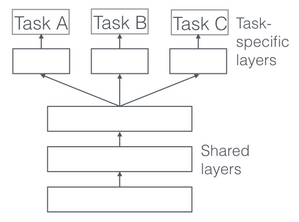
\includegraphics[width=.6\textwidth]{hard.png}
        \caption{Hard parameter sharing}
        \label{fig:hard}
    \end{subfigure}
    \hfill
    \begin{subfigure}[t]{0.48\textwidth}
        \centering
        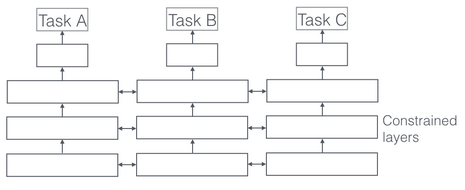
\includegraphics[width=\textwidth]{soft.png}
        \caption{Soft parameter sharing}
        \label{fig:soft}
    \end{subfigure}
    \caption{\cite{ruderOverviewMultiTaskLearning2017}}
    \label{}
\end{figure}

Another approach of conditioning the tasks is the family of feature-wise transformations. In this approach, we can have three different transformations, a) the concatenation, b) the addition, and c) the multiplication. These transformations can be applied in a layer-wise manner, allowing for more flexibility in how tasks are integrated into the model. They can be incorporated either at the initial input of the architecture or at a later stage of the generation process. For the concatenation, given a representation of a task, $z$, (e.g. one-hot encoded), the input of a layer is concatenated with $z$, and the output is their linear transformation. For the addition and the multiplication, the conditioning representation is linearly transformed and then added and multiplied to the input respectively. For all these methods, the operations are applied element-wise, hence the name feature-wise transformations \cite{dumoulin2018feature-wise}.


\begin{figure}[h!]
    \centering
    \begin{subfigure}[t]{0.48\textwidth}
        \centering
        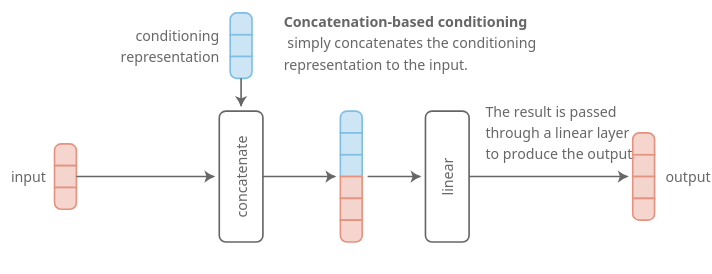
\includegraphics[width=\textwidth]{concat.png}
        \caption{Concatenation}
        \label{}
    \end{subfigure}
    \hfill
    \begin{subfigure}[t]{0.48\textwidth}
        \centering
        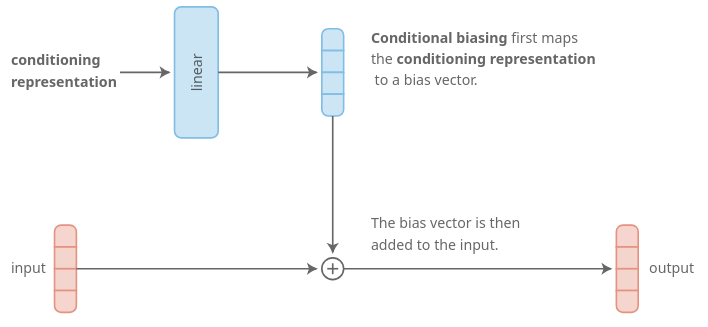
\includegraphics[width=\textwidth]{add.png}
        \caption{Addition}
        \label{}
    \end{subfigure}
    \begin{subfigure}[b]{.48\textwidth}
        \centering
        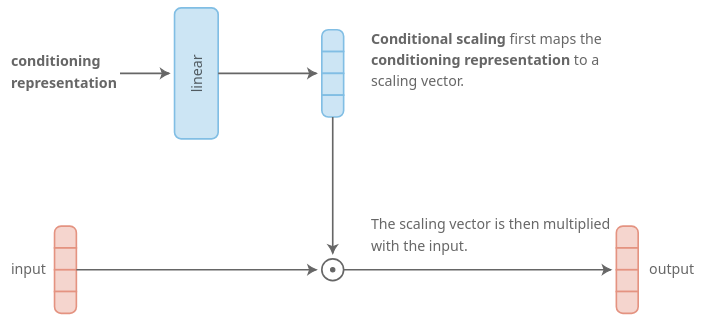
\includegraphics[width=\textwidth]{mul.png}
        \caption{Multiplication}
        \label{}
    \end{subfigure}    
    \caption{Methods of integrating conditioning representation \cite{ruderOverviewMultiTaskLearning2017}}
    \label{}
\end{figure}

Broadly speaking, \gls{mlt} methods can be categorized along several dimensions, including the learning paradigm (e.g., supervised or unsupervised), the type of tasks (e.g., classification or regression), and the nature of the input space. In this work, we focus primarily on supervised tasks, which also represent the most widely studied setting in the \gls{mlt} literature \cite{zhangSurveyMultiTaskLearning2021}.
As we will explore in the next section, our primary task of interest is the prediction of gene expression profiles following a perturbation, which can be formulated as a regression problem. The input consists of a cell’s baseline (or "vehicle") gene expression profile, and the output corresponds to the gene expression profile after the perturbation is applied. The perturbation itself is represented by a condition vector, typically implemented as a one-hot encoding that specifies the type of perturbation administered to the cell.

Formally speaking, for supervised tasks with the same input space, we can define $m$ learning tasks $\{T_{i}\}_{i=1}^m$, and $\mathcal{D}_i$ as the accompanying dataset for the $i$th task, consisting of $n_i$ samples, i.e., $\mathcal{D}_i = \left\{(x_j^i, y_j^i)\right\}_{j=1}^{n_i}$, where $x_j^i$ is the $j$th input sample and $y_j^i$ is its corresponding label.
The loss for the $i$th task can be formulated as $\mathcal{L}_i(\{\theta_i, \theta_{sp}\}, \mathcal{D}_i)$, where $\theta_i$ are the task-specific parameters and $\theta_{sp}$ are the shared parameters.
The goal of \gls{mlt} is to learn a set of parameters $\theta$ that minimizes the total loss across all tasks, i.e.,

\[
\theta = \arg\min_{\theta} \sum_{i=1}^m \mathcal{L}_i(\theta_i, \mathcal{D}_i)
\]

, where $\theta = \{\theta_{sp}, \theta_1, \dots, \theta_m\}$ represents the total set of model parameters.
% 


\section{Perturbation modeling objectives}

In the field of perturbation modeling, there are four main objectives that can be outlined \cite{gavriilidisMinireviewPerturbationModelling2024, jiMachineLearningPerturbational2021, heumos2023best}.

The prediction of unseen omics signatures and phenotypic changes after a perturbation is applied to either a cell line (bulk omics) or individual cells (single-cell omics) is considered the primary objective, often referred to as Out-of-Distribution (OOD). Regarding omics signatures, scGen is a well-known model that has served as a baseline for perturbed single-cell transcriptomics prediction. For phenotypic changes, this could refer to cell viability as a function of drug dosage, typically quantified by IC50 values. DeepDSC \cite{li2019deepdsc} is another example, a deep neural network that predicts the drug sensitivity of cancer cell lines based on their gene expression profiles and a compound descriptor. This compound descriptor is represented as Morgan fingerprints\footnote{Morgan fingerprints, also known as extended-connectivity fingerprints (ECFP), are a type of molecular fingerprint used in cheminformatics to represent the structure of molecules in a computer-readable format. They encode the structural features into a binary vector \cite{morgan1965generation}}, capturing the 1D and 2D structure of the compound.

%The second objective is related to the prediction of the mode-of-action of the perturbation. This could entail predicting the pathway mechanisms and the target proteins that will be activated or inhibited by the perturbation. Understanding to what kind of proteins a drug can bind to and the cascade events triggered by this interaction is fundamental for drug discovery and repurposing. DeepDTAGen, is a multi-task model, that is able to predict the biding affinity of a drug to a protein, and to generate new drug candidates, represented with SMILES strings \footnote{SMILES stands for Simplified Molecular Input Line Entry System. It's a way to represent a chemical molecule as a text string using ASCII characters. For example, ethanol (CH₃CH₂OH) can be represented as the string "CCO"}, based on a target protein \cite{shah2025deepdtagen}.


The second objective concerns the prediction of a perturbation's mode of action. This involves identifying the signaling pathways and specific target proteins that are activated or inhibited in response to a given perturbation. Understanding which proteins a drug interacts with, and the downstream cascade of molecular events it initiates, is fundamental for drug discovery and repurposing.
DeepDTAGen \cite{shah2025deepdtagen} is a multi-task model designed to address this challenge. It predicts the binding affinity between a drug and a target protein, and also generates novel drug candidates represented as SMILES strings\footnote{SMILES stands for Simplified Molecular Input Line Entry System. It is a text-based representation of molecular structures. For example, ethanol (CH₃CH₂OH) can be represented as the string "CCO" in SMILES format.}, conditioned on a given protein target.

Perturbation interaction prediction, that can be highly beneficial for combinatorial treatments, is treated as the third objective. The goal is to predict how different perturbations interact with each other, which is crucial for understanding drug-drug interactions and potential interlinked side effects. This can involve predicting whether two drugs will have synergistic or antagonistic effects when administered together. For example, the DeepSynergy model predicts a synergy score having as inputs the gene expression profiles of a cell line and the chemical descriptors of two drugs \cite{preuer2018deepsynergy}. The synergy score quantifies the deviation of an experimentally observed response surface from one predicted by a theoretical reference model, such as Loewe Additivity \cite{loewe1953problem}, Bliss Independence \cite{bliss1939toxicity}, Highest Single Agent (HSA) \cite{tan2012systematic}, or the more recent Zero Interaction Potency (ZIP) \cite{yadav2015searching}.
% I could elaborate more on the last ones, what is loewe additivity and such

The fourth objective involves the prediction of chemical properties. For instance, the task can be formulated to design de novo chemical compounds that can induce a desired perturbed gene expression profile. PerturbNet \cite{yuPerturbNetPredictsSinglecell2022} is a model capable of addressing this challenge. It first compresses the feature spaces of both transcriptomic profiles and chemical structures using autoencoders. These two modalities are then linked via a conditional invertible neural network (cINN).
By operating the cINN in reverse, the model enables counterfactual predictions, allowing the exploration of the chemical feature space for perturbations likely to produce a specified gene expression response. In this way, the task serves as a conceptual bridge between biology and chemistry, linking molecular structure to phenotypic effect.

\section{Multi-task learning and perturbation modeling}

As mentioned by \cite{jiMachineLearningPerturbational2021,gavriilidisMinireviewPerturbationModelling2024}, \gls{mlt} can be considered a powerful ML/DL approach that can be promising to be applied for perturbation modeling. It is worth mentioning that for the NCI-DREAM challenge \cite{costello2014community}, addressing the drug sensitivity of unseen cell lines, a Bayesian \gls{mlt} approach was considered to perform the best \cite{schrod2024codex}. 

In addition to the categorization of perturbation modeling objectives, single-cell analysis tasks, such as gene regulatory network (GRN) inference, cell clustering, and multi-modal integration, can be highly beneficial when incorporated into a \gls{mlt} framework. These tasks provide complementary biological context that can enhance the performance and interpretability of perturbation modeling.
For example, UnitedNet \cite{tangExplainableMultitaskLearning2023} has demonstrated strong performance in cross-modal prediction and cell-type classification by leveraging multi-omics data within an \gls{mlt} architecture. Similarly, ScPreGAN \cite{weiScPreGANDeepGenerative2022} integrates cell type classification as an auxiliary task to improve the generation of perturbed single-cell transcriptomic profiles, illustrating the value of combining single-cell tasks with perturbation modeling objectives.

Solving multiple tasks together can be challenging when they operate on different levels of granularity. For example, prediction of cell viability or drug sensitivity with IC50 values is considered a population-level task, while prediction of single-cell gene expression after a perturbation is a cell-level task. For the former, available datasets provide information about the gene expression profiles of cell lines, along with the chemical compound and the corresponding IC50 values. However, for single-cell perturbation response prediction, a corresponding population-level phenotype (like IC50) from the same experiment is often not directly available. Solving these tasks simultaneously would require bridging bulk with single-cell omics, taking into account the technical variations between the experimental procedures of data acquisition.

On the other hand, the task of predicting bulk-level perturbation responses could be integrated with other population-level tasks such as cell viability, drug sensitivity, synergy prediction, and target/pathway prediction. Datasets that could provide the required information for this bulk analysis by intersecting cell lines include the LINCS L1000 \cite{subramanian2017next} dataset, which consists of 689,831 microarray measurements from 170 different cell lines treated with 20,065 compounds; the Genomics of Drug Sensitivity in Cancer (GDSC) \cite{iorio2016landscape}, which catalogues genomic profiles of 639 human cancer cell lines and their drug response data to 130 drugs; and the large-scale oncology screen produced by Merck \& Co. \cite{o2016unbiased}, which includes 23,062 samples, where each sample consists of two compounds and a cell line.

Instead of treating perturbation objectives as independent tasks, the objectives themselves can be formulated within a \gls{mlt} framework. For example, by defining the prediction of gene expression for a particular perturbation as a task, \gls{mlt} is implicitly utilized by models such as scVIDR \cite{kanaGenerativeModelingSinglecell2023} and CODEX \cite{schrod2024codex}. These models aim to perform this task across multiple perturbations using the same model and by encoding the perturbation as a conditional signal. Another example of division of a specific perturbation objective is STAMP \cite{gaoSubtaskDecompositionbasedLearning2024}, a multi-task model that predicts the differential effect of a perturbation relative to the control gene expression profile. To achieve this, three tasks have been identified: a) which genes are differentially expressed, b) the magnitude of the differential expression, and c) the direction of the differential expression. The model is trained to predict these three tasks simultaneously, allowing for a more comprehensive understanding of the perturbation effect.


% Aside from this categorization of perturbation modeling objectives, there could be other ways of task definition that can lead to the usage of multi-task learning. For example, single, multiple perturbations.

% There have been several instances that multi-task learning has been implicitly or explicitly applied, involving single-cell tasks as well.
% - UnitedNet
% - scpregan uses cell type classification 
% - bayesian multi task won the challenge
% - codex solves for multiple perturbations
% - scvidr as well
% - mlt in drug design paper
% - stamp paper
% should I mention how would be possible to solve simultaneously a task and its reversed task? For example, given an omics signature predict something, and given a perturbed omics signature predict the chemical compound used. Isn't this a class since the prediction of the second is the condition to predict the first? But cinn is something that could work for this.

%sequential, parallel, soft, hard parameter sharing

\section{Method}

Based on the previous analysis of potential integration of perturbation objectives, emphasis has been given to the single-cell 
use case, as it has been the most explored in the literature due to the recent advancements of single-cell technology. More specifically, we define the prediction of the unseen single-cell gene expression after a perturbation is applied as a task, and we will explore designing a model that can achieve this for a set of perturbations. Similarly to the drug-protein study \cite{allenspach2024neural}, where the prediction of the binding affinity between a drug and a protein corresponds to a different task for each protein, we will treat each perturbation as a separate task. 

% why the perturbation has been integrated not at the input but the decoder? 

% some models are able to predict for unseen perturbation, not only unseen cell, this should mention, and why we followed this approach, the mlt for drug design is the case that the model can for unseen cell and unseen perturbation.


%Inspired by the drug-target multi task setup as well.

\begin{wrapfigure}{r}{0.5\textwidth}
  \begin{center}
    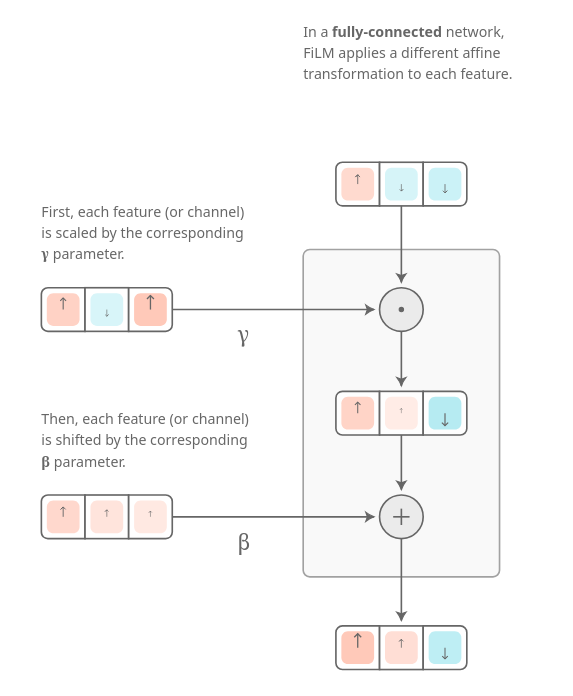
\includegraphics[width=0.48\textwidth]{film_layers.png}
  \end{center}
  \caption{Illustration of the FiLM transformation \cite{dumoulin2018feature-wise}}
\end{wrapfigure}

About the conditioning of the task, as we have seen at \cref{sec:mlt}, we have explored the application of conditional affine transformation, a combination of multiplicative and additive conditioning, that shifts and scales the input element-wise. It is efficient in terms of scaling and parameters compared to multi-head architectures, where each task has its dedicated network to generate the output of the task . This approach is named as FiLM, for Feature-wise Linear Modulation \cite{dumoulin2018feature-wise, perez2018film}:

\[ \text{FiLM(x)} = \gamma (z) \odot x + \beta (z) \]

, where $\gamma$, and $\beta$ are learnable parameters generated by the so called FiLM generator, that takes as input a condition $z$ (e.g. a vector that indicates the task), and $x$ is the input to be transformed. 
A FiLM layer is the application of the FiLM transformation to the input of a layer, where the parameters $\gamma$ and $\beta$ can be generated by a common or layer-specific FiLM generator.   Then the result of the transformation is propagated to the rest of the network.

% \begin{figure}[h!]
%     \centering
%     \begin{subfigure}[t]{0.48\textwidth}
%         \centering
%         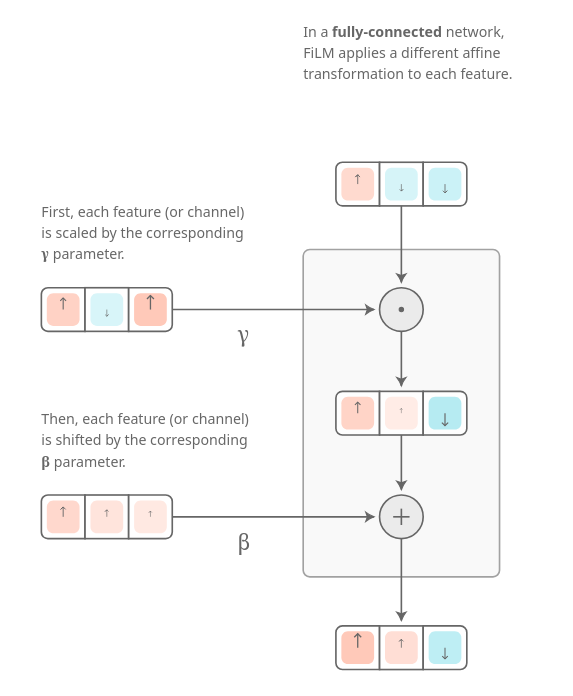
\includegraphics[width=\textwidth]{film_layers.png}
%         \caption{Illustration of the FiLM layer}
%         \label{}
%     \end{subfigure}
%     \hfill
%     \begin{subfigure}[t]{0.48\textwidth}
%         \centering
%         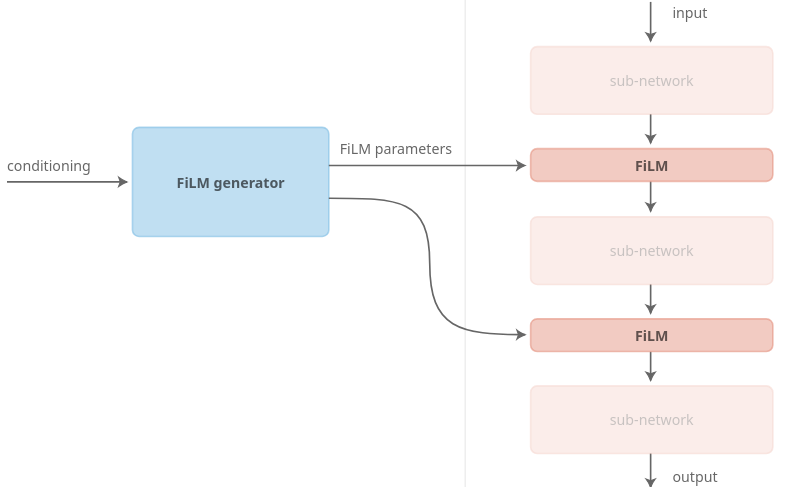
\includegraphics[width=\textwidth]{film_gen.png}
%         \caption{A common FiLM generator used across FiLM layers}
%         \label{}
%     \end{subfigure}
%     \caption{Illustration of the FiLM \cite{dumoulin2018feature-wise}}
%     \label{fig:film}
% \end{figure}

% \begin{figure}[h!]
%     \centering
%     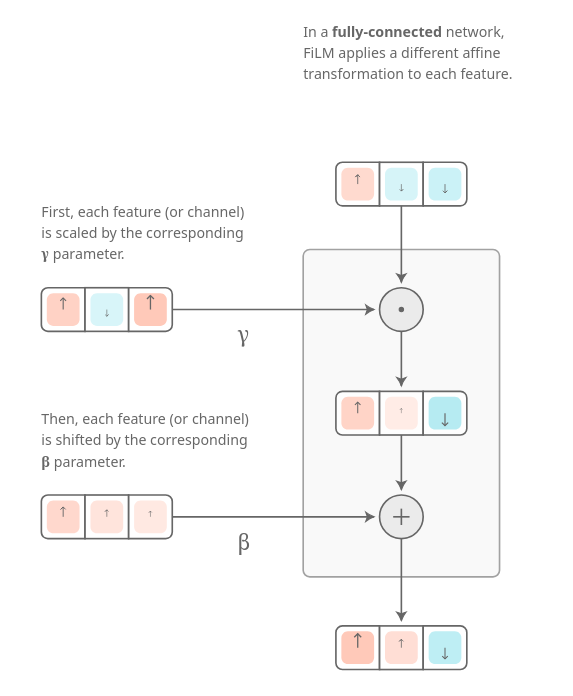
\includegraphics[width=0.5\textwidth]{film_layers.png}
%     \caption{Illustration of the feature-wise transformation \cite{dumoulin2018feature-wise}}
%     \label{fig:film}
% \end{figure}

In our approach, we aim to decouple the perturbation effect by constructing a perturbation-free latent space, while explicitly modeling the perturbation response through a conditioning signal that represents the type of perturbation. Our baseline architecture is built around an autoencoder, and this conditioning signal is integrated via FiLM layers fused into the decoder (\verb|MTAe|), named as \verb|MTAe|. The modulation parameters $\gamma$ and $\beta$ are learned independently for each fusion point with a dedicated FiLM generator.

During training, the model learns to reconstruct the perturbed gene expression profiles from the control profiles, while the FiLM layers modulate the decoder's hidden layers based on the perturbation type.
The loss is the reconstruction loss of the autoencoder, which is the mean squared error between the input and the output of the decoder:
\[
\mathcal{L}_{\text{recon}} = \frac{1}{N} \sum_{i=1}^{N} ||x_i - \hat{x}_i||^2 \]
, where $x_i$ and $\hat{x}_i$ are the input and the reconstructed gene expression profile respectively, and $N$ is the number of samples.
% I could mention why the condition isn't integrated at the first layers?


We hold out the stimulated samples of the cell type of interest as the test set. The control samples of that cell type, along with both control and stimulated samples from all other cell types, are used for training. The perturbation is represented as a one-hot encoded vector, where, for a dataset with N perturbations, the conditioning vector has length N+1, with an extra entry representing the control condition. This setup enables the model to generalize to the effect of known perturbations on a new, unseen cell type.

\begin{figure}
    \centering
    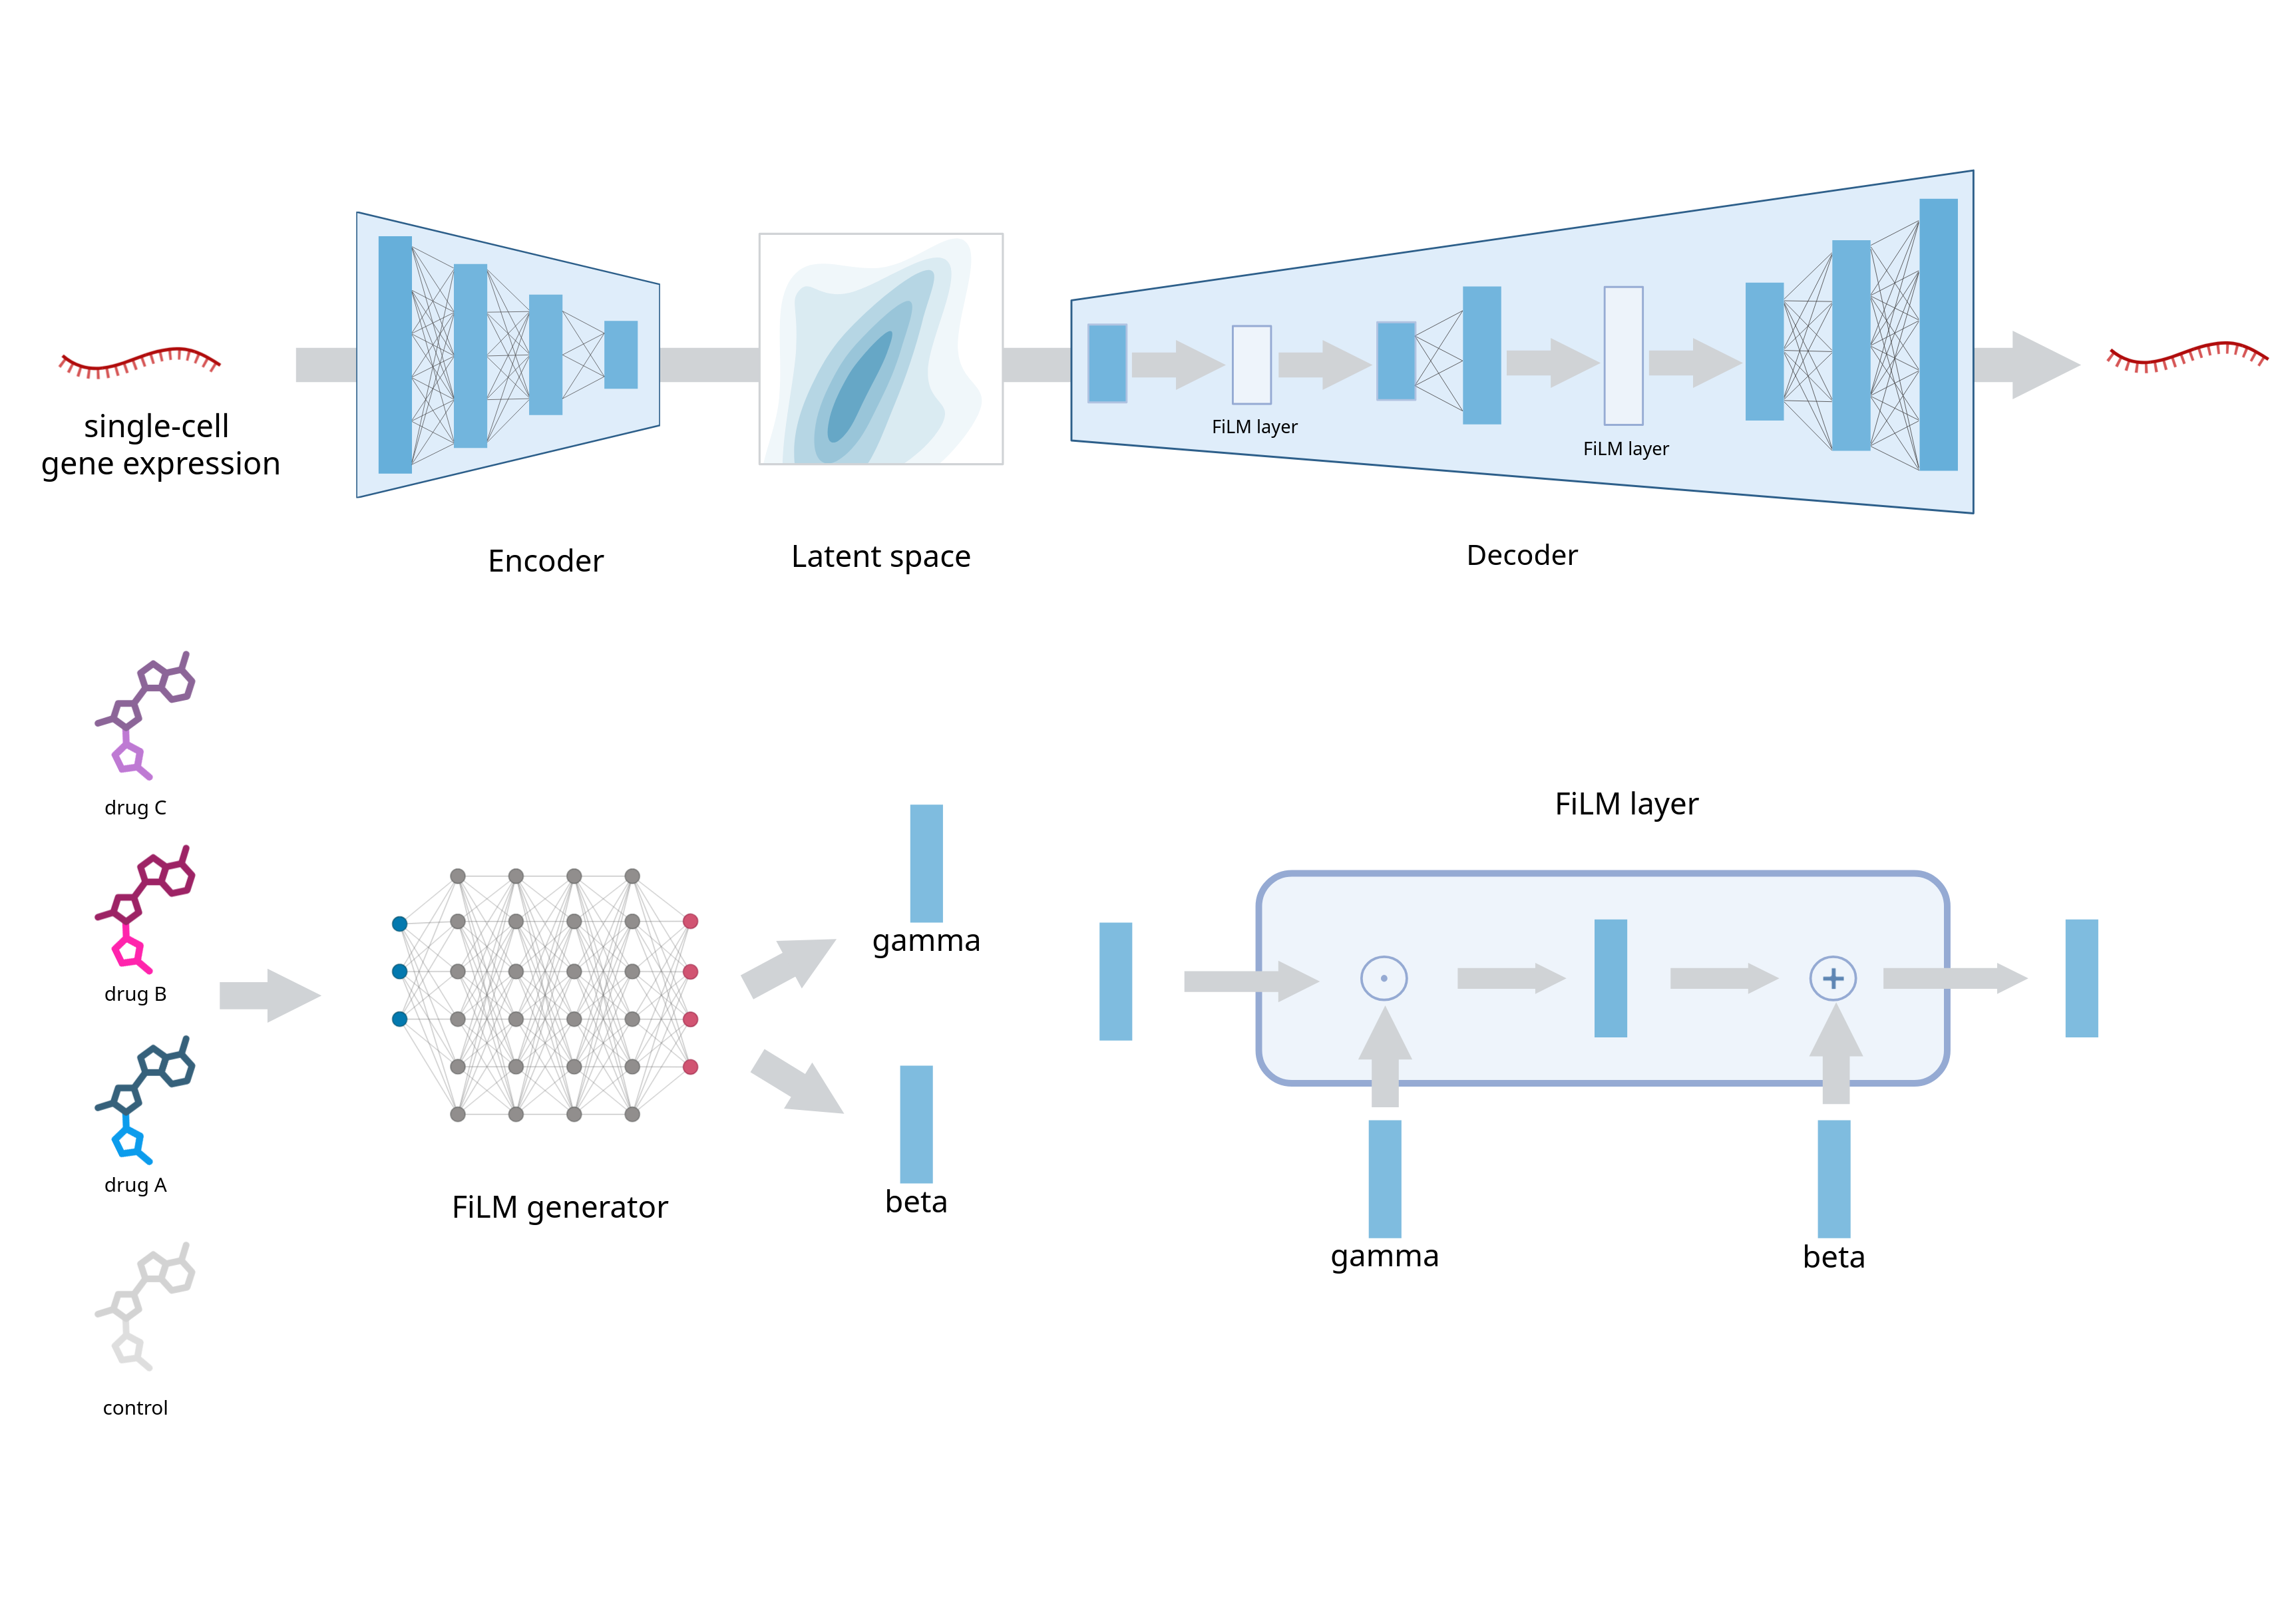
\includegraphics[width=\textwidth]{biorender_film_architecture.png}
    \caption{Illustration of the multi-task architecture. The encoder is shared across all tasks, while the decoder is conditioned by the task-specific FiLM layers. In this example, only two film layers are integrated in the first two hidden layers of the decoder. The FiLM generator takes as input a conditioning representation of the perturbations (e.g. one-hot encoded), and outputs the modulation parameters $\gamma$, and $\beta$ for the FiLM layers. Created in  \url{https://BioRender.com}}
\end{figure}
% I have to document the losses


We have explored several variations of this approach, all of which maintain the decoder architecture with the inclusion of FiLM-based conditioning for all the hidden layers of the decoder. These variations can be split to three main groups, a) adversarial autoencoders, b) optimal transport, c) Variational Autoencoders (VAEs).

\subsection{Adversarial autoencoders (AeAdv)}

In our adversarial autoencoder variations, we enforce structure in the latent space via an adversarial loss. The architecture builds on the previously described autoencoder with FiLM layers, extended with a discriminator. The discriminator is trained to distinguish between encoded latent vectors and samples from a target distribution, while the encoder is trained adversarially to fool the discriminator. This encourages the latent space to match the desired target distribution.

In the \verb|MTAeAdv| architecture, we aim to explicitly model a perturbation-free latent space. Here, the discriminator is trained to distinguish between latent representations of control and perturbed gene expression profiles, while the encoder attempts to make them indistinguishable. This encourages the latent space to be agnostic to perturbation.

In contrast, the \verb|MTAeAdvG| architecture enforces a Gaussian prior on the latent space. The discriminator differentiates between latent vectors from the encoder and samples from a fixed multivariate Gaussian, while the encoder learns to match this distribution.

The total loss for the adversarial autoencoder is a combination of the reconstruction loss and the adversarial loss, defined as:
\[\mathcal{L}_{\text{Adv}} = (1 - \lambda) \mathcal{L}_{\text{recon}} +  \lambda \mathcal{L}_{\text{adv}}\]
, where $\lambda$ is a hyperparameter that controls the trade-off between reconstruction and adversarial loss, and $\mathcal{L}_{\text{adv}}$ is the adversarial loss, which can be defined as the binary cross-entropy loss between the discriminator's predictions and the true labels (1 for real samples, 0 for generated samples):
\[\mathcal{L}_{\text{adv}} = -\frac{1}{N} \sum_{i=1}^{N} \left[ y_i \log(D(z_i)) + (1 - y_i) \log(1 - D(z_i)) \right]\]
, where $D(z_i)$ is the discriminator's prediction for the $i$th latent vector $z_i$, and $y_i$ is the true label (1 for control, 0 for perturbed).

% \begin{figure}
%     \centering
%     \begin{subfigure}[t]{0.48\textwidth}
%         \centering
%         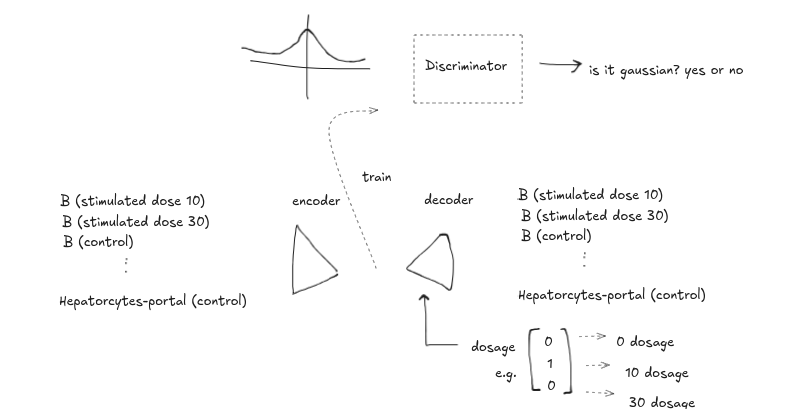
\includegraphics[width=\textwidth]{ae_gauss_sketch.png}
%         \caption{}
%         \label{}
%     \end{subfigure}
%     \hfill
%     \begin{subfigure}[t]{0.48\textwidth}
%         \centering
%         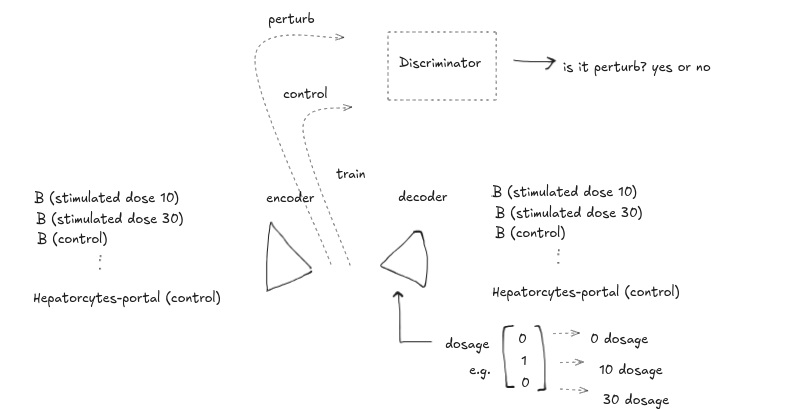
\includegraphics[width=\textwidth]{ae_adv_sketch.png}
%         \caption{}
%         \label{}
%     \end{subfigure}
%     \caption{Adversarial autoencoders}
%     \label{}
% \end{figure}

\subsection{Optimal transport (OT)}

Another set of architectural variations incorporates optimal transport to address the lack of paired samples in single-cell RNA sequencing. Because the same cell cannot be sequenced both before and after a perturbation, we lack true one-to-one correspondences between control and perturbed conditions. As a result, modeling must rely on comparing distributions rather than individual cell-level changes.

To mitigate this, we use optimal transport to approximate correspondences between distributions. Specifically, for a given sample from the control distribution, a matching sample from the perturbed distribution is assigned based on OT. This pseudo-pairing allows us to reformulate the training objective: instead of reconstructing the input (as in a standard autoencoder), the model is trained to map control cells to their OT-matched counterparts in the perturbed distribution.

The loss is the mean squared error between the input and the output of the decoder, defined as:

\[
\mathcal{L}_{\text{OT}} = \frac{1}{N} \sum_{i=1}^{N} ||x_i - \hat{x}_i||^2 
\]

, where $x_i$ is the input gene expression profile, $\hat{x}_i$ is the paired perturbed gene expression profile, and $N$ is the number of samples. 

Compared to the previous architectures, the perturbed gene expression profiles aren't used as inputs to be reconstructed. Instead, they are used as a target distribution to be mapped given the control gene expression profile and the type of the perturbation. This approach is named as \verb|MTAeOT|. Additionally, we have attempted to pretrain the model with the \verb|MTAe| architecture and then fine-tune it with the \verb|MTAeOT| architecture. This approach is named as \verb|MTAePlusOT|.

% \begin{figure}
%     \centering
%     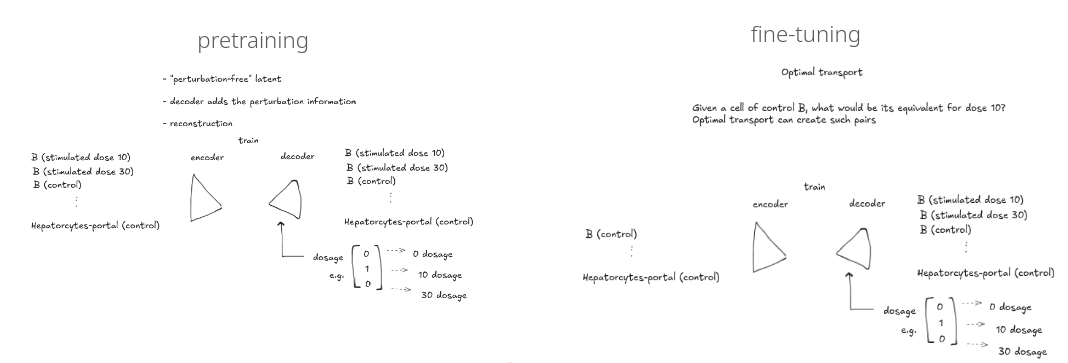
\includegraphics[width=\textwidth]{ae_ot_sketch.png}
%     \caption{Using optimal transport to fine-tune the MTAe architecture (MTAePlusOT)}
% \end{figure}

\subsection{Variational Autoencoder (VAE)}

The last set of variations involves the inclusion of \gls{vae}. The architecture builds upon the previously described autoencoder framework augmented with FiLM layers, while additionally incorporating a VAE loss to regularize the latent space. The VAE loss is defined as the sum of the reconstruction loss and the Kullback--Leibler (KL) divergence between the learned latent distribution and a standard normal prior:

\[
\mathcal{L}_{\text{VAE}} = \mathbb{E}_{q_\phi(z|x)}[\log p_\theta(x|z)] - D_{\text{KL}}(q_\phi(z|x) \,\|\, p(z))
\]

Here, $q_\phi(z|x)$ is the encoder's approximation of the posterior over latent variables, $p_\theta(x|z)$ is the decoder's likelihood of reconstructing the input, and $p(z) \sim \mathcal{N}(0, I)$ is the prior over latent variables. This model is named as \verb|MTVae|, and as we have described above with the optimal transport use case, we have the \verb|MTVaeOT| and \verb|MTVaePlusOT| architectures.

% \begin{figure}
%     \centering
%     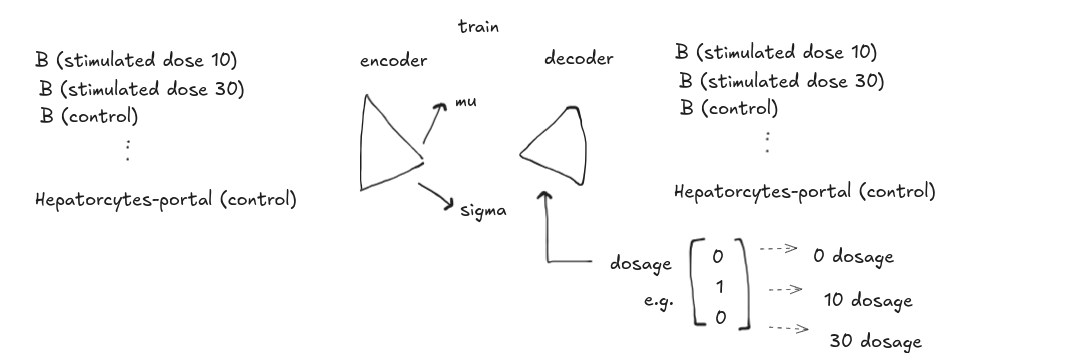
\includegraphics[width=0.8\textwidth]{vae_sketch.png}
%     \caption{VAE}
% \end{figure}


\section{Current single-cell perturbation modeling methods}

In the literature body, there are several approaches for predicting single-cell perturbation responses. An overview of the models on perturbation modeling can be found on this study \cite{gavriilidisMinireviewPerturbationModelling2024}. To compare our multi-task method, we have chosen the models of scGen \cite{lotfollahiScGenPredictsSinglecell2019}, scVIDR \cite{kanaGenerativeModelingSinglecell2023}, scPreGAN \cite{weiScPreGANDeepGenerative2022}, and scButterfly \cite{caoScButterflyVersatileSinglecell2024}.
One of the key tasks for these models is out-of-distribution detection. A typical dataset for this task consists of transcriptomic profiles obtained from single-cell sequencing technologies (scRNA-seq) from multiple cell types in both control and perturbed conditions. The objective is to predict the perturbed gene expression profile of a held-out (unseen) cell type, given its control-state profile. To achieve this, the model must learn the perturbation effect from the remaining cell types in both conditions. The performance of all of these models will serve as a baseline to evaluate our multi-task learning architectures.

\subsection{scGen}

scGen's architecture is based on a \gls{vae} that learns a probabilistic latent space representation of the gene expression profiles. 
The perturbation effect is modeled as a vector $\delta$, calculated as the mean of the differences between the latent vectors of the perturbed and control gene expression profiles. Then, the latent perturbed gene expression profile of a held-out cell type, $\hat{z}$,  is generated by adding this perturbation vector, $\delta$, to the latent vector of the control profile, $z$, using $\hat{z} = z + \delta$. Finally, the perturbed gene expression is obtained by decoding the generated latent vector, $\hat{z}$, using the decoder of the \gls{vae}. This approach allows for the generation of new perturbed profiles by manipulating the latent space representation using vector arithmetic.

\subsection{scVIDR}
 

A key limitation of scGen is the absence of explicit cell-type-specific modeling, which can reduce its ability to generalize to unseen cell types with distinct perturbation responses.
scVIDR addresses this by incorporating cell-type-aware perturbation estimation. Rather than computing a single global perturbation vector $\delta$ based only on the condition labels, scVIDR fits a linear regression model that captures how perturbation vectors vary across cell types.
For each training cell type $i$, the perturbation vector is defined as $\delta_i = \hat{z}_i - z_i$,
where $z_i$​, and $\hat{z}_i$ are the mean latent representation of the control, and perturbed cells of type $i$ respectively.
A linear model is then trained to predict $\hat{\delta}_i$​ from $z_i$, i.e., $\hat{\delta}_i = f(z_i)$.


Once trained, this model can predict the perturbation vector $\delta_A$​ for an unseen cell type $A$, using only its control-state latent representation $z_A$, i.e., $\hat{\delta}_A = f(z_A)$.
This cell-type-aware prediction improves generalization by allowing the model to tailor the perturbation response based on the control-state context of each cell type.

scVIDR can also predict the gene expression profile for multiple dosages. Similarly, scVIDR fits a linear regression model to predict the perturbation vector $\hat{\delta}_c$ across cell types, but in this case, the conditions are the lowest and the highest dosage. Intermediate dosages are then calculated by log linearly interpolating on the $\hat{\delta}_c$.

Regarding interpretability, the bottleneck of the non-linear mapping from the latent space to the gene expression space is replaced by a linear one, utilizing a sparse linear regression model. This is approximated by a weight matrix $\hat{W}_{VAE}$, with dimensions $MxG$ where $M$ is the number of latent variables and $G$ is the number of genes. Then this matrix is used to examine the contribution of the latent variables to the gene expression profile, using the following equation:

\[\text{gene score} = \hat{\delta}_c^T \hat{W}_{VAE}\]

A higher gene score indicates a bigger change at the expression level of the gene if the dosage increases.

\subsection{scPreGAN}

scPreGAN integrates an autoencoder with a \gls{gan} framework to predict single-cell RNA-seq (scRNA-seq) data under perturbations. The architecture consists of a shared encoder and two generators, one for each condition (control and perturbed). To align the generated distributions with the real data, the model employs two discriminators, each associated with a specific condition.

The encoder, which is shared across both conditions, learns a perturbation-free latent representation that captures high-level biological features common to both states. The generators then incorporate condition-specific perturbation effects to reconstruct the gene expression profiles from the latent space. The discriminators are trained to distinguish between real and generated samples, while the generators are optimized adversarially to produce realistic reconstructions that fool their respective discriminators.


\subsection{scButterfly}


scButterfly is a generative adversarial model built on a dual-aligned \gls{vae} architecture, designed for cross-modal translation in single-cell data. The model has demonstrated strong performance in translating between transcriptomic and chromatin accessibility profiles, as well as between transcriptomic and proteomic data.

Its architecture consists of two \gls{vae}s, each pretrained on a specific modality, and a translator component that aligns the latent spaces of the two encoders. The translator is composed of two neural networks, one per modality, each modeling a Gaussian distribution in the latent space. These networks take the encoder's latent representation as input, sample from the modeled distribution, and pass the sample to the decoder of the other modality, enabling cross-modal generation.
After VAE pretraining, the translator is trained to align the latent spaces such that biologically meaningful translation across modalities can be achieved.

Although scButterfly isn't primarily designed for perturbation modeling, the study has demonstrated its potential, by treating control and perturbed expression profiles as two modalities. One of its limitations is the narrow evaluation scope, as it has been tested only on the case of human \gls{pbmc} stimulated by interferon beta (IFN-b) \cite{kanaGenerativeModelingSinglecell2023}.

\section{Evaluation}

%Regarding data splitting, we hold of the stimulated samples of the cell type of interest as a test set. The controlled ones, along with the rest of the cell types in both conditions of control and stimulated, are used for training. The model is evaluated on the unseen cell type, given as input the control gene expression \cref{fig:umap_side_by_side}. The performance is measured by comparing the predicted gene expression with the actual one.

% I should mention preprocessing

We have tested the models on two datasets, one where human peripheral blood mononuclear cells have been stimulated by IFN-b interferon (Kang et al. \cite{kanaGenerativeModelingSinglecell2023}), and a multi-perturbation dataset, where liver cells have been stimulated by multiple doses of tetrachlorodibenzo-p-dioxin (TCDD) in vivo (Nault et al. \cite{nault2021single,nault2022benchmarking}).

The models are evaluated on the unseen cell type, given as input the control gene expression \cref{fig:umap_side_by_side}.
Regarding the single perturbation response models, the scGen, scButterfly, scPreGAN and scVIDR's single-task version, for the multi-perturbation dataset of ten dosages Nault et.al \cite{nault2021single,nault2022benchmarking}, we have trained a dedicated model for each dosage. In these cases, the dataset is consisted of only two conditions the control and the perturbed one for a particular dosage. The performance is measured by comparing the predicted gene expression with the actual one.

For this comparison, we have used the count of differentially expressed genes (DEGs), the $R^2$ of all the highly variable genes (HVGs), and the top 100 most variable ones. To complement the evaluation, we have calculated a set of five distance metrics (euclidean, edistance, wasserstein, mean pairwise, mmd) to capture the differences between the expected and predicted perturbed gene expressions in a point-wise and distributional manner using pertpy \cite{heumos2024pertpy}.

To address the randomness of the models, we have performed the experiments three times, with three different seeds 1, 2, 19193, and the metrics have been averaged across experiments.

To rank the models, since there could be conflicting cases between metrics, where one model could be better than the other, per model's metric we averaged them across all the experiments. Then we scaled them to the range of 0-1 with the following formula:

\[\frac{\text{current} - \text{best}}{\text{worst} - \text{best}}\]

% it could be reversed if highest is better

, that can track how a metric deviates from the best one. Then we summed all the metrics, giving a score (penalty) to each model. The model with the lowest score is considered the best one.

\begin{figure}[h!]
    \centering
    \begin{subfigure}[t]{0.48\textwidth}
        \centering
        \includegraphics[width=\textwidth]{figures/nault_umap_split_multiple.png}
        \caption{Nault et al. \cite{nault2021single,nault2022benchmarking}}
        \label{fig:nault_umap}
    \end{subfigure}
    \hfill
    \begin{subfigure}[t]{0.48\textwidth}
        \centering
        \includegraphics[width=\textwidth]{figures/pbmc_split.png}
        \caption{Kang et al. \cite{kanaGenerativeModelingSinglecell2023}}
        \label{fig:pbmc_umap}
    \end{subfigure}
    \begin{subfigure}[b]{0.48\textwidth}
        \centering
        \includegraphics[width=\textwidth]{figures/nault_umap_split_30.png}
        \caption{Example of single dose split of Nault et al. \cite{kanaGenerativeModelingSinglecell2023} for the dosage $30 \mu g/kg$}
        \label{fig:pbmc_umap}
    \end{subfigure}    
    \caption{UMAP representations of data split}
    \label{fig:umap_side_by_side}
\end{figure}

% \begin{figure}[h!]
%     \centering
%     \includegraphics[width=.7\textwidth]{figures/nault_umap_split_multiple.png}
%     \caption{Nault et al. \cite{nault2021single,nault2022benchmarking}}
%     \label{fig:nault_umap}
% \end{figure}

% \begin{figure}[h!]
%     \centering
%     \includegraphics[width=.7\textwidth]{figures/pbmc_split.png}
%     \caption{Kang et al. \cite{kanaGenerativeModelingSinglecell2023}}
%     \label{fig:pbmc_umap}
% \end{figure}

\clearpage

\section{Results}

Initially, we will benchmark only our multi-task variations to filter out the most promising models \cref{fig:selected_pbmc_baseline,fig:selected_pbmc_distance,fig:selected_nault_cell_type_baseline,fig:selected_nault_cell_type_distance,fig:selected_nault_doses_baseline,fig:selected_nault_doses_distance}.
As we can see the best performing ones are MTAe, MTAeAdv, and MTAeAdvG. Thus, we will compare them with state-of-the-art literature models such as scButterfly, scVIDR, scPreGAN and scGen.

scVIDR performance drops for DEGs, and distance metrics, but it performs well for the $R^2$ metrics and stays very consistent, along with scGEN. The multi-task models and scButterfly exhibit greater variability across measurements, but better performance on average. The optimal transport variations performed poorly overall, but were among the best for distance metrics for the Nault et al. \cite{nault2021single,nault2022benchmarking} dataset. 

% model & DEGs & $R^2_{\text{HVG}}$ & $R^2_{\text{HVG20}}$ & $R^2_{\text{HVG100}}$ & Euc & Was & E-dist & MPD & MMD \\

\begin{figure}[h!]
    \centering
    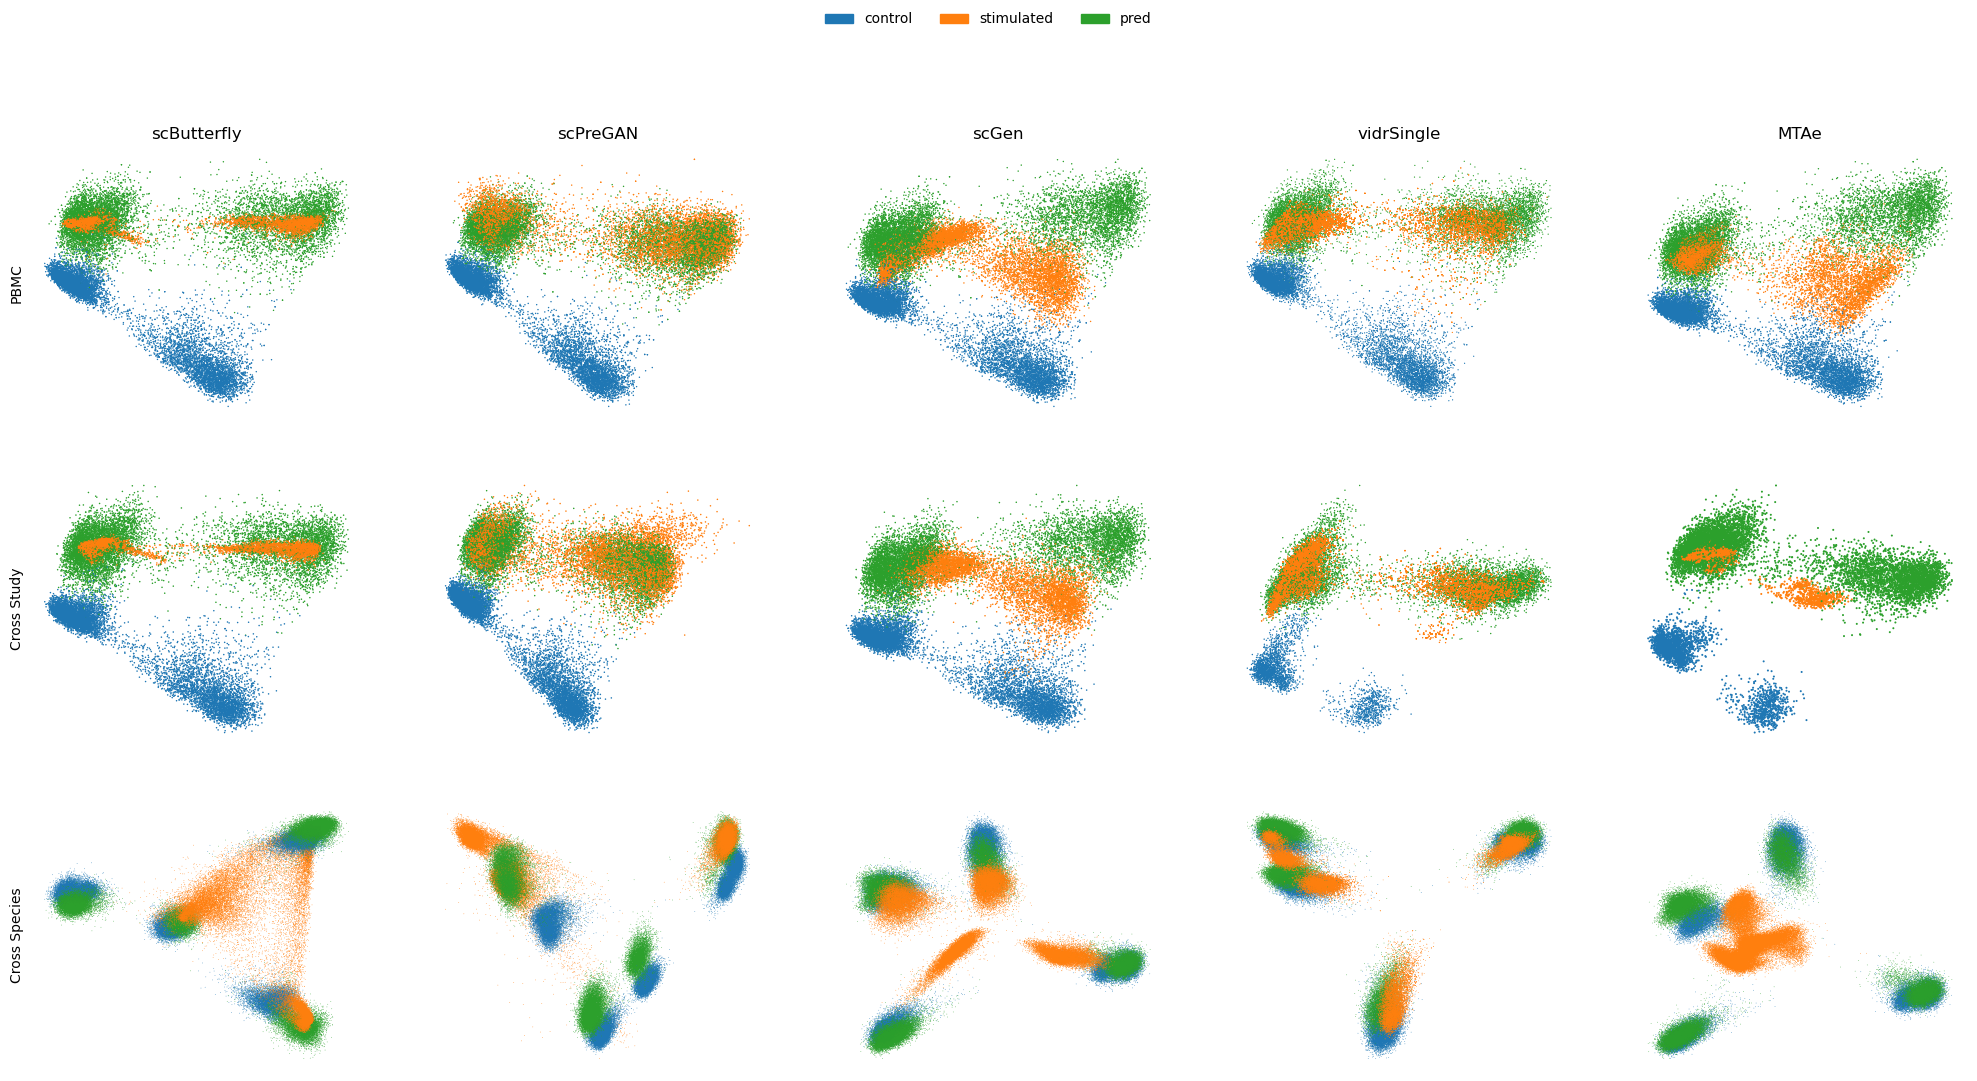
\includegraphics[width=\textwidth]{pcas.png}
    \caption{PCA dimensionality reduction of the real unperturbed data, the real perturbed data and the predicted perturbed data.}
    \label{fig:selected_nault_cell_type_baseline}
\end{figure}

\clearpage

\subsection{Kang et al.}


\begin{table}[h!]
    \centering
    \scalebox{0.8}{
    \begin{tabularx}{\textwidth}{lXXXXXXXXX}
    \toprule
    model & DEGs & $R^2_{\text{HVG}}$ & $R^2_{\text{HVG20}}$ & $R^2_{\text{HVG100}}$ & Euc & Was & E-dist & MPD & MMD \\
    \midrule
    MTAe & \textbf{0.000 (75.714)} & 0.077 (0.946) & 0.330 (0.871) & 0.140 (0.917) & 0.479 (0.488) & 0.815 (0.892) & 0.506 (0.651) & 0.898 (0.949) & 0.479 (0.488) \\
    MTAeAdv & 0.066 (72.381) & 0.026 (0.961) & 0.053 (0.955) & 0.043 (0.948) & 0.032 (0.202) & 0.006 (0.604) & 0.044 (0.429) & 0.110 (0.800) & 0.032 (0.202) \\
    MTAeAdvG & 0.195 (65.905) & 0.168 (0.917) & 0.305 (0.878) & 0.192 (0.901) & 0.503 (0.504) & 0.636 (0.828) & 0.570 (0.681) & 0.689 (0.909) & 0.503 (0.504) \\
    MTAeOT & 0.688 (41.190) & 1.000 (0.657) & 1.000 (0.668) & 1.000 (0.648) & 0.984 (0.811) & 0.969 (0.947) & 0.990 (0.883) & 0.976 (0.963) & 0.984 (0.811) \\
    MTAePlusOT & 0.768 (37.190) & 0.960 (0.670) & 0.983 (0.674) & 0.970 (0.657) & 0.982 (0.810) & 0.982 (0.951) & 0.983 (0.880) & 0.988 (0.966) & 0.982 (0.810) \\
    MTVae & 0.132 (69.095) & 0.088 (0.942) & 0.056 (0.954) & 0.105 (0.928) & 0.125 (0.261) & 0.056 (0.621) & 0.189 (0.499) & 0.114 (0.800) & 0.125 (0.261) \\
    MTVaeOT & 0.720 (39.571) & 0.961 (0.669) & 0.969 (0.678) & 0.953 (0.663) & 0.988 (0.813) & 0.993 (0.955) & 0.990 (0.883) & 0.992 (0.966) & 0.988 (0.813) \\
    MTVaePlusOT & 0.899 (30.619) & 0.987 (0.661) & 0.994 (0.670) & 0.976 (0.655) & 1.000 (0.821) & 1.000 (0.958) & 1.000 (0.888) & 1.000 (0.968) & 1.000 (0.821) \\
    scButterfly & 0.299 (60.727) & 0.251 (0.891) & 0.187 (0.914) & 0.232 (0.889) & 0.140 (0.271) & \textbf{0.000 (0.601)} & 0.128 (0.469) & \textbf{0.000 (0.779)} & 0.140 (0.271) \\
    scGen & 0.868 (32.143) & 0.191 (0.910) & 0.326 (0.872) & 0.290 (0.870) & 0.697 (0.627) & 0.863 (0.909) & 0.744 (0.765) & 0.885 (0.946) & 0.697 (0.627) \\
    scPreGAN & 0.796 (35.750) & 0.634 (0.771) & 0.376 (0.857) & 0.518 (0.799) & 0.496 (0.499) & 0.248 (0.690) & 0.572 (0.682) & 0.381 (0.851) & 0.496 (0.499) \\
    vidrSingle & 1.000 (25.536) & \textbf{0.000 (0.970)} & \textbf{0.000 (0.971)} & \textbf{0.000 (0.961)} & \textbf{0.000 (0.182)} & 0.014 (0.606) & \textbf{0.000 (0.408)} & 0.096 (0.797) & \textbf{0.000 (0.182)} \\
    \bottomrule
    \end{tabularx}}
    \caption{Score of the models for Kang et al. \cite{kanaGenerativeModelingSinglecell2023} along with the actual value in parenthesis}
\end{table}



\begin{table}[h!]
    \centering
    \scalebox{0.8}{    
    \begin{tabular}{lrrr}
    \toprule
    model & score & baseline score & distance score \\
    \midrule
    MTAeAdv & 0.414099 & 0.188957 & 0.225142 \\
    MTVae & 0.989313 & 0.381226 & 0.608087 \\
    vidrSingle & 1.109933 & 1.000000 & 0.109933 \\
    scButterfly & 1.375249 & 0.968395 & 0.406855 \\
    MTAe & 3.723979 & 0.546259 & 3.177721 \\
    MTAeAdvG & 3.762873 & 0.860886 &
     2.901987 \\
    scPreGAN & 4.519561 & 2.325642 & 2.193919 \\
    scGen & 5.559246 & 1.674543 & 3.884703 \\
    MTVaeOT & 8.552051 & 3.602547 & 4.949504 \\
    MTAeOT & 8.590746 & 3.688019 & 4.902727 \\
    MTAePlusOT & 8.598116 & 3.680466 & 4.917650 \\
    MTVaePlusOT & 8.855812 & 3.855812 & 5.000000 \\
    \bottomrule
    \end{tabular}}
    \caption{Kang et al. \cite{kanaGenerativeModelingSinglecell2023}}
\end{table}
    

\begin{figure}[h!]
    \centering
    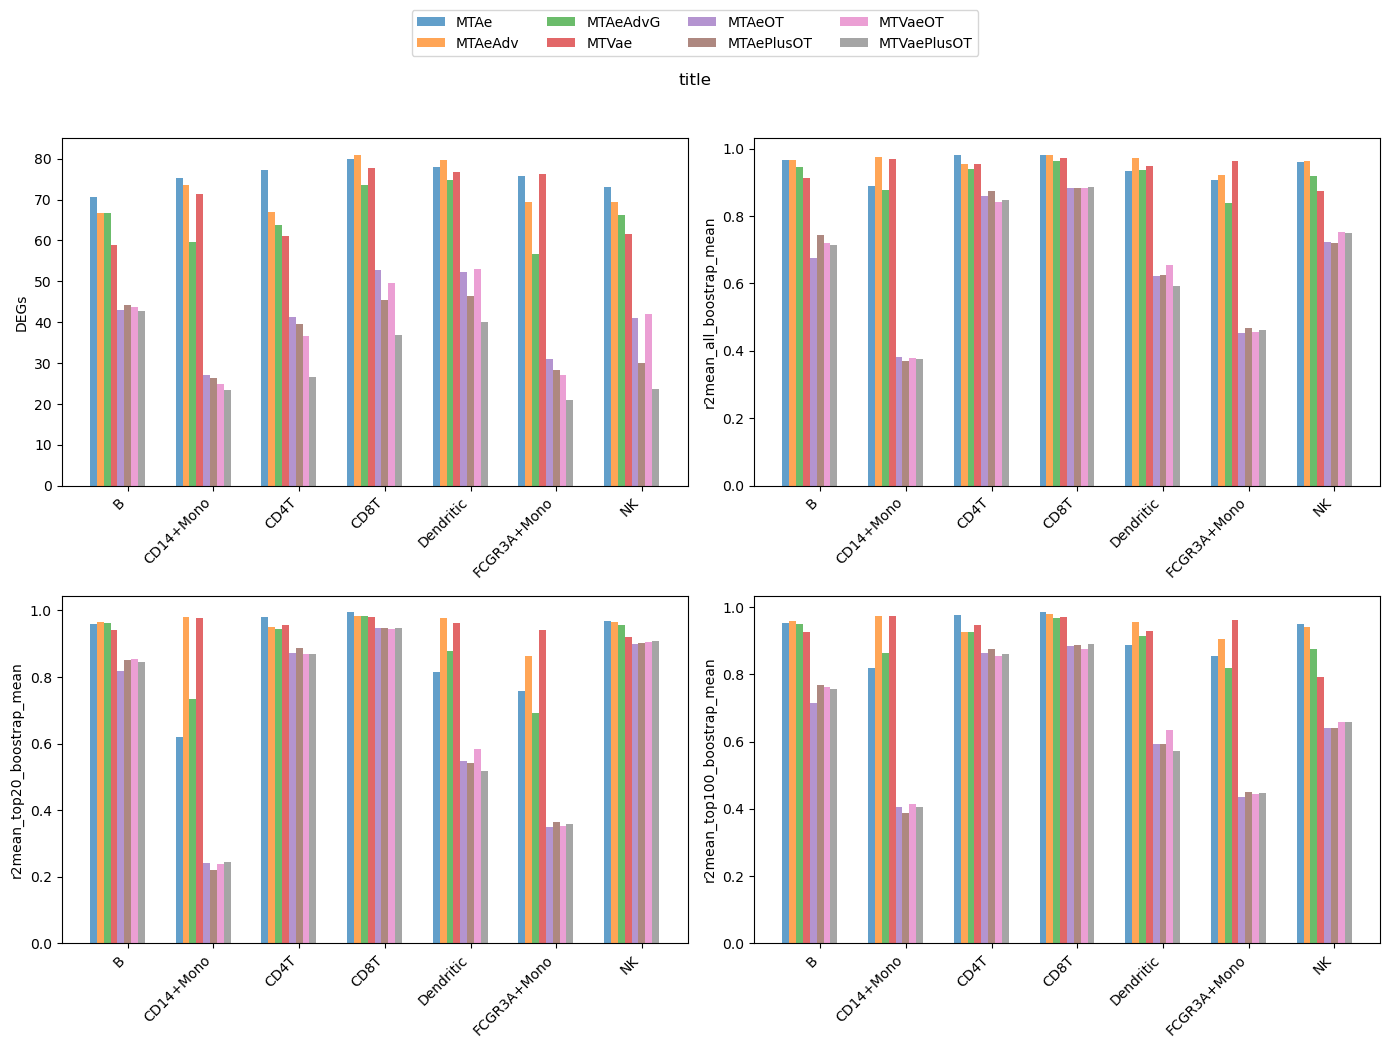
\includegraphics[width=.85\textwidth]{multi_task_benchmarking_cell_type_baseline_metrics_pbmc.png}
    \caption{Baseline metrics of multi-task models for the Kang et al. \cite{kanaGenerativeModelingSinglecell2023} dataset across cell types}
\end{figure}

\begin{figure}[h!]
    \centering
    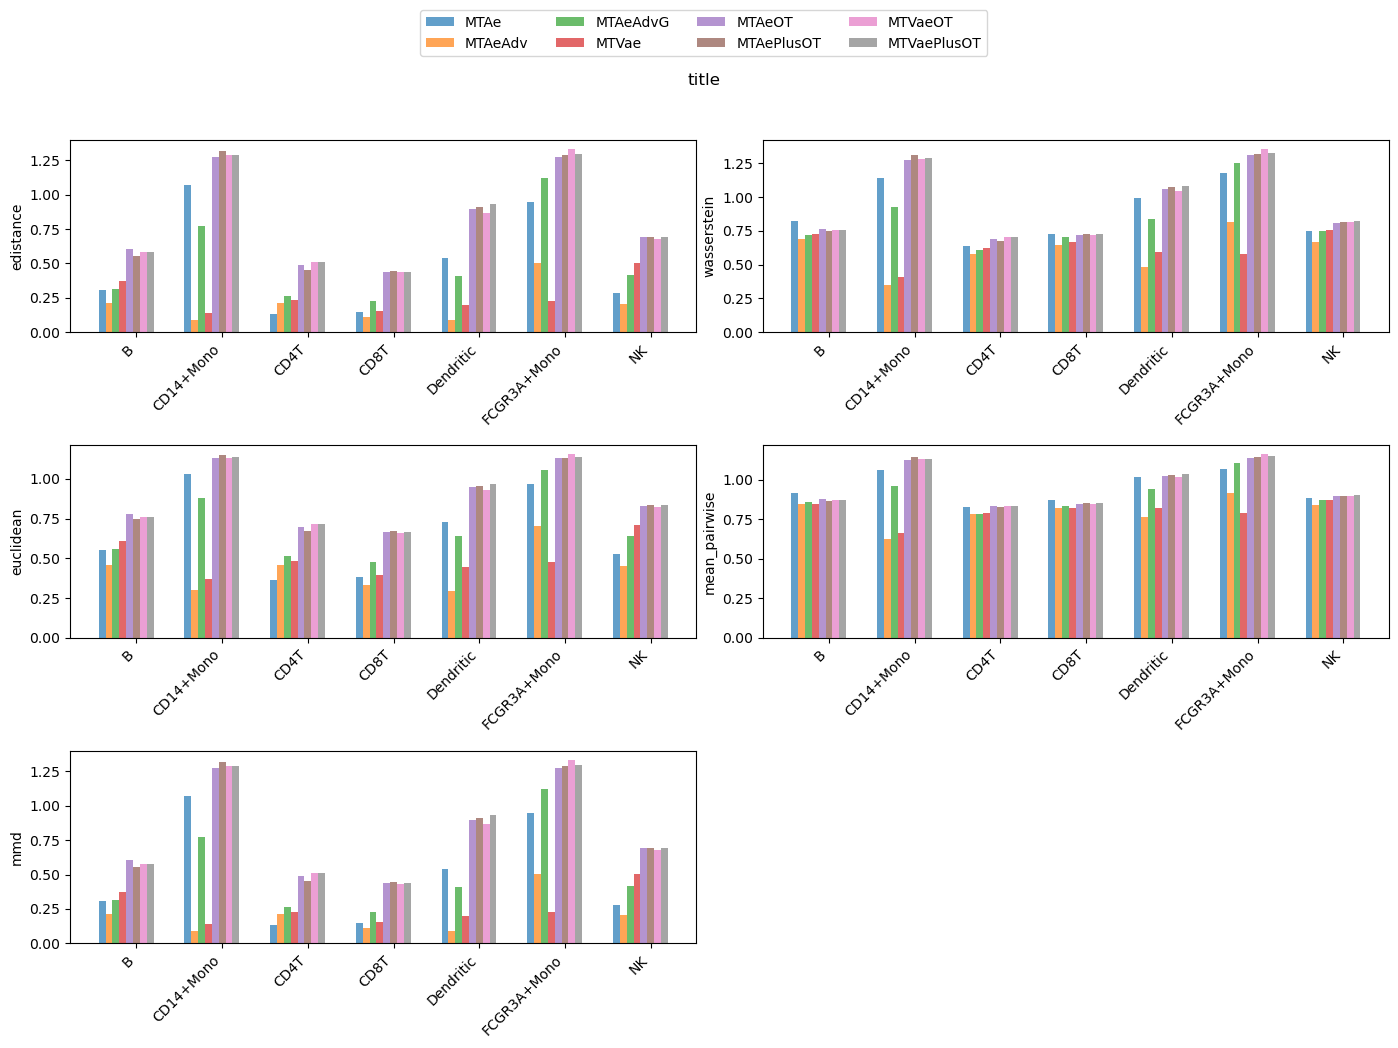
\includegraphics[width=.85\textwidth]{multi_task_benchmarking_cell_type_distance_metrics_pbmc.png}
    \caption{Distance metrics of multi-task models for the Kang et al. \cite{kanaGenerativeModelingSinglecell2023} dataset across cell types}
\end{figure}

\begin{figure}[h!]
    \centering
    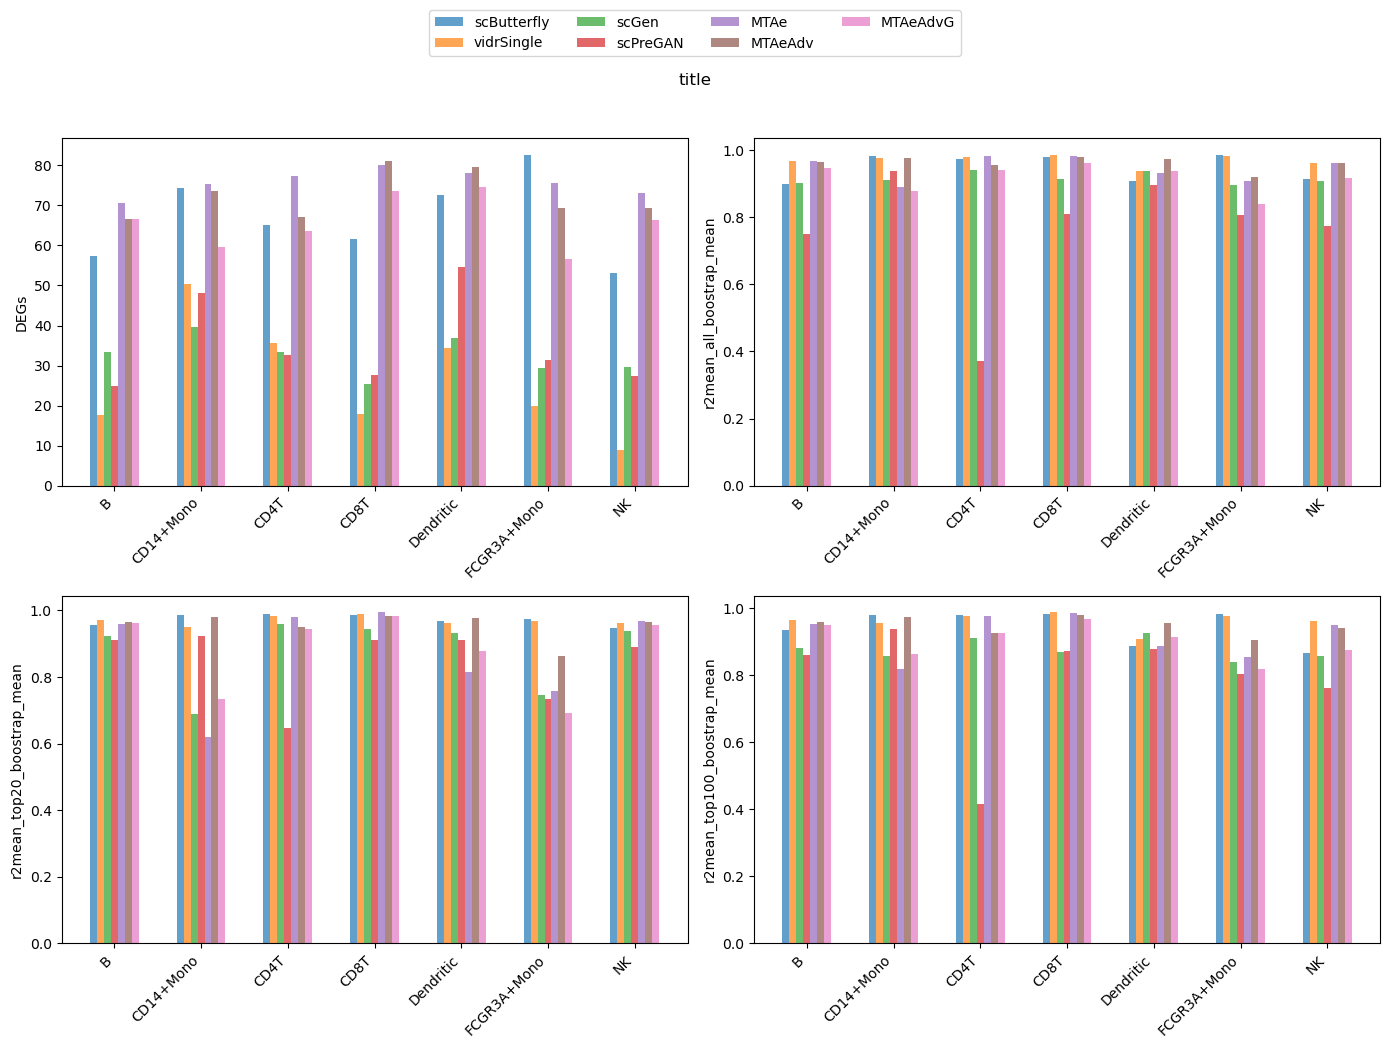
\includegraphics[width=.85\textwidth]{selected_benchmarking_cell_type_baseline_metrics_pbmc.png}
    \caption{Baseline metrics of multi-task and literature models for the Kang et al. \cite{kanaGenerativeModelingSinglecell2023} dataset across cell types}
    \label{fig:selected_pbmc_baseline}
\end{figure}

\begin{figure}[h!]
    \centering
    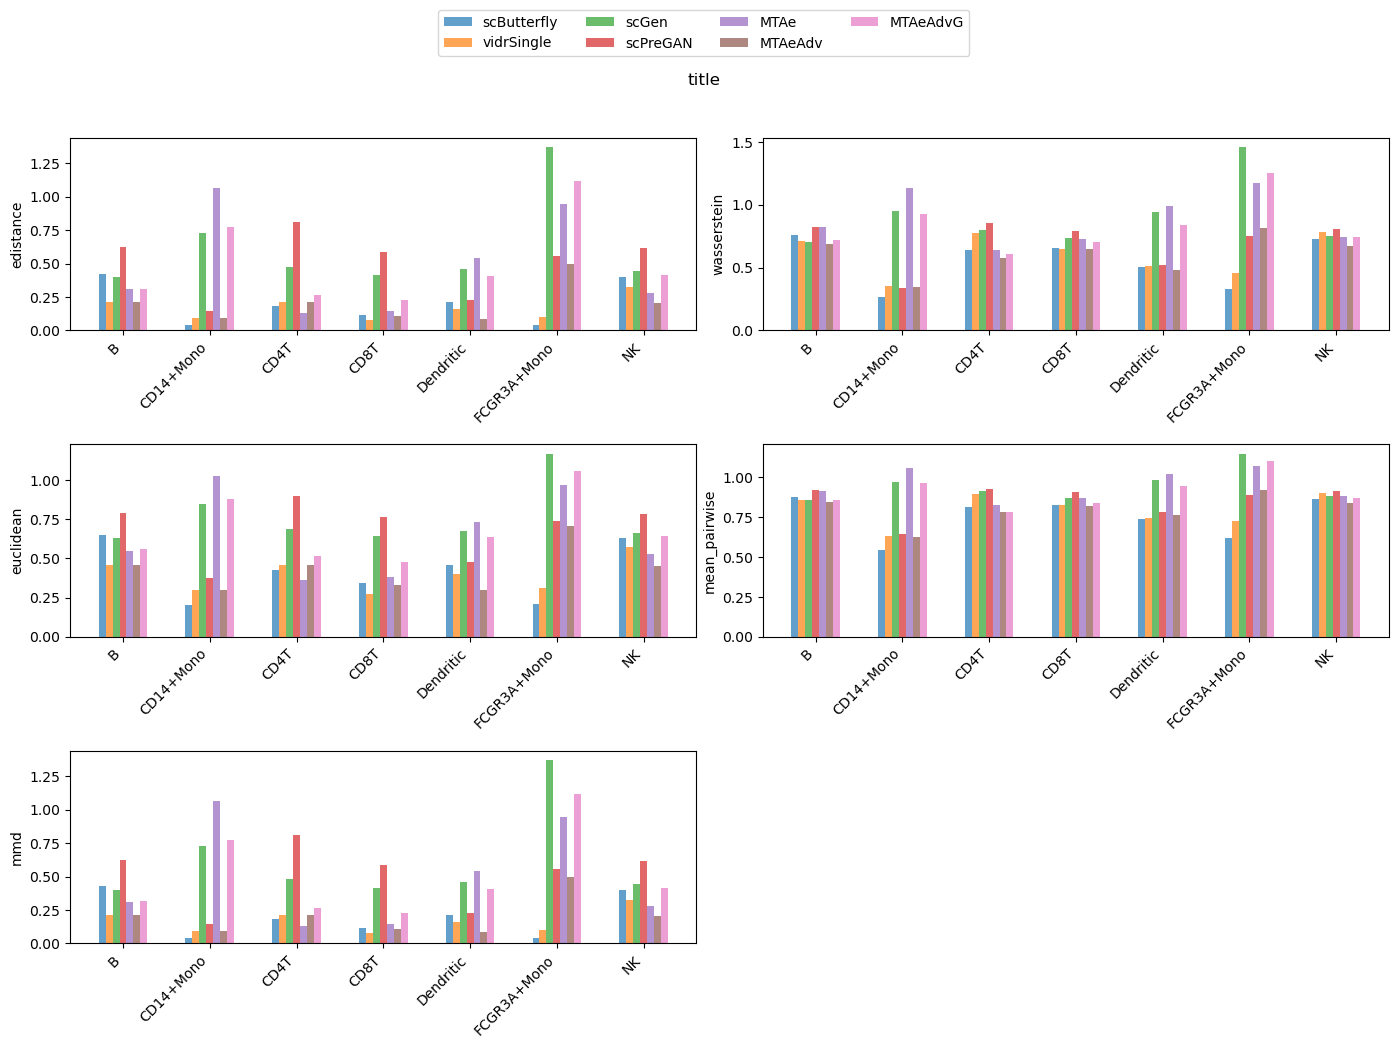
\includegraphics[width=.85\textwidth]{selected_benchmarking_cell_type_distance_metrics_pbmc.png}
    \caption{Distance metrics of multi-task and literature models for the Kang et al. \cite{kanaGenerativeModelingSinglecell2023} dataset across cell types}
    \label{fig:selected_pbmc_distance}
\end{figure}

\begin{figure}[h!]
    \centering
    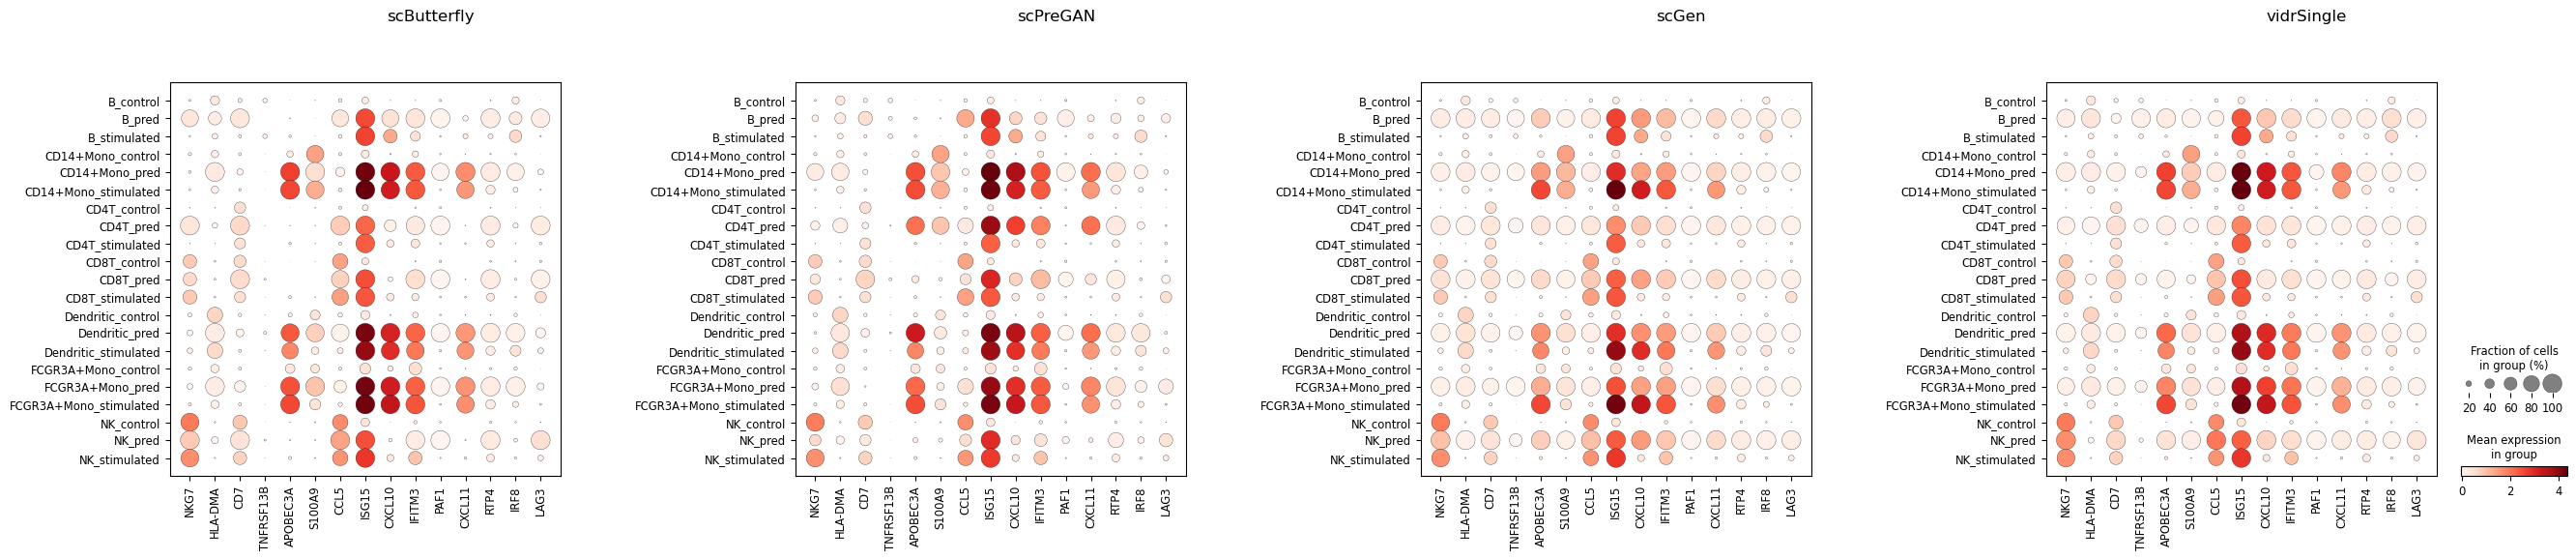
\includegraphics[width=.85\textwidth]{dotplots_literature_pbmc.png}
    \caption{}
    \label{fig:selected_pbmc_distance}
\end{figure}

\begin{figure}[h!]
    \centering
    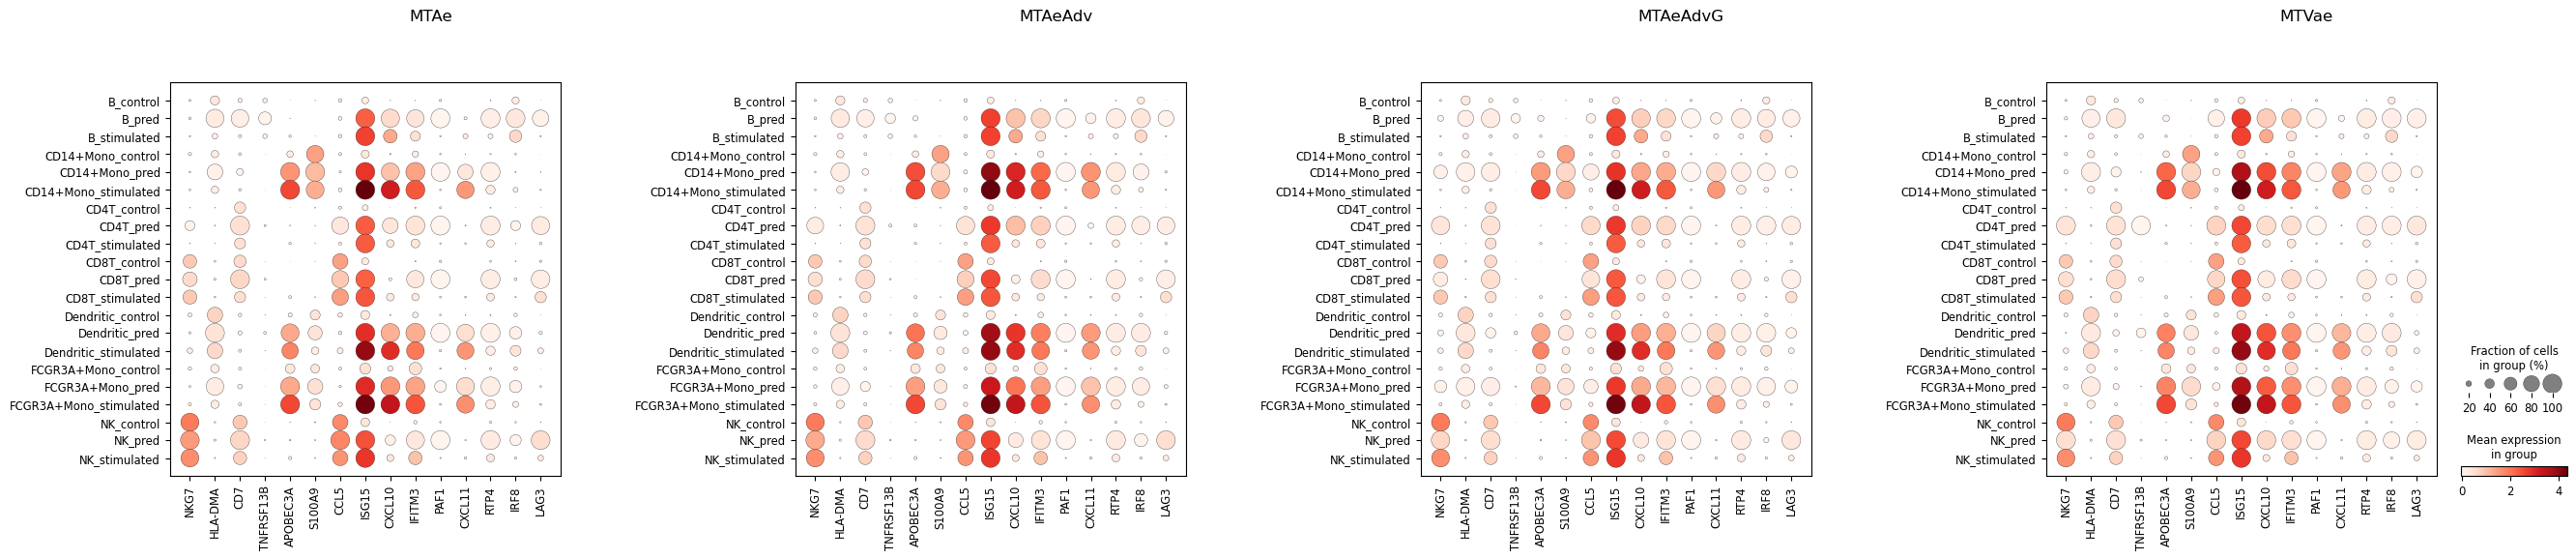
\includegraphics[width=.85\textwidth]{dotplots_multitask1_pbmc.png}
    \caption{}
    \label{fig:selected_pbmc_distance}
\end{figure}

\begin{figure}[h!]
    \centering
    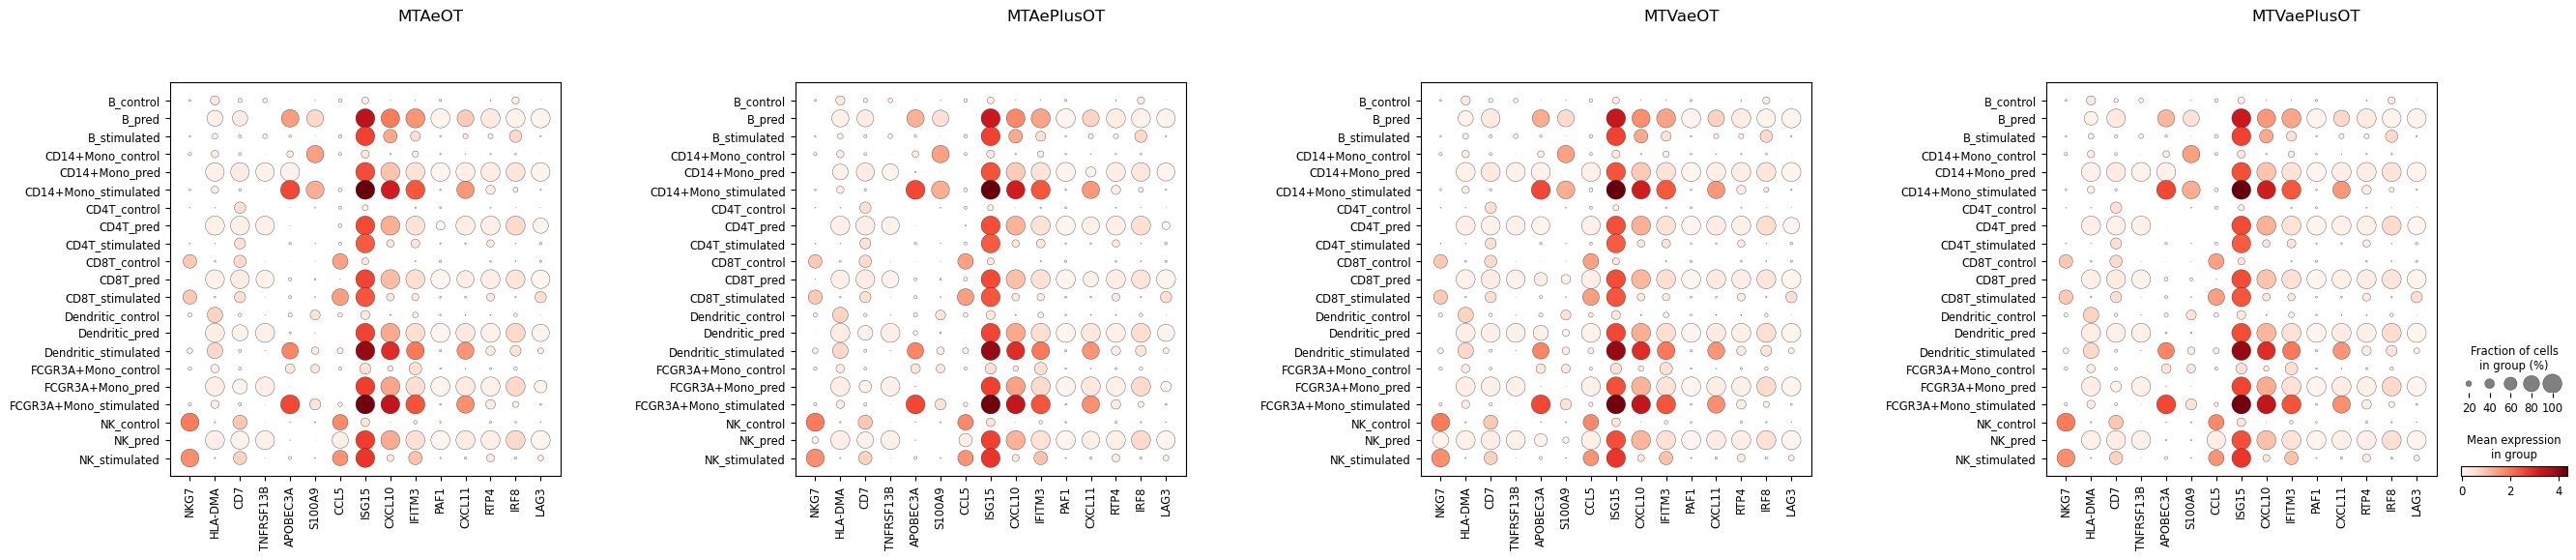
\includegraphics[width=.85\textwidth]{dotplots_multitask2_pbmc.png}
    \caption{}
    \label{fig:selected_pbmc_distance}
\end{figure}

\begin{figure}[h!]
    \centering
    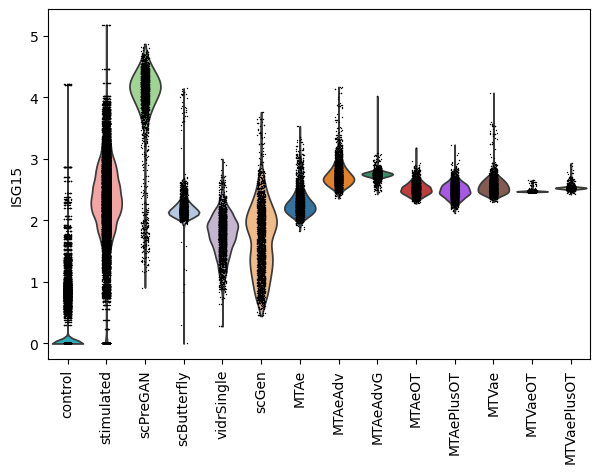
\includegraphics[width=.85\textwidth]{violins_pbmc.png}
    \caption{}
    \label{fig:selected_pbmc_distance}
\end{figure}


\clearpage

\subsection{Cross-study}

\begin{table}[h!]
    \centering
    \scalebox{0.8}{
    \begin{tabularx}{\textwidth}{lXXXXXXXXX}
    \toprule
    model & DEGs & $R^2_{\text{HVG}}$ & $R^2_{\text{HVG20}}$ & $R^2_{\text{HVG100}}$ & Euc & Was & E-dist & MPD & MMD \\
    \midrule
    MTAe & 0.066 (64.048) & 0.224 (0.902) & 0.369 (0.882) & 0.223 (0.904) & 0.446 (0.344) & 0.733 (0.794) & 0.528 (0.538) & 0.746 (0.876) & 0.446 (0.344) \\
    MTAeAdv & 0.166 (59.000) & 0.161 (0.922) & 0.277 (0.906) & 0.158 (0.922) & 0.228 (0.210) & 0.383 (0.610) & 0.337 (0.436) & 0.347 (0.773) & 0.228 (0.210) \\
    MTAeAdvG & 0.230 (55.762) & 0.227 (0.901) & 0.393 (0.876) & 0.217 (0.906) & 0.382 (0.305) & 0.563 (0.704) & 0.476 (0.510) & 0.558 (0.828) & 0.382 (0.305) \\
    MTAeOT & 0.674 (33.381) & 1.000 (0.658) & 1.000 (0.720) & 1.000 (0.687) & 0.992 (0.683) & 0.964 (0.916) & 1.000 (0.789) & 0.970 (0.934) & 0.992 (0.683) \\
    MTAePlusOT & 0.893 (22.333) & 0.945 (0.675) & 0.961 (0.730) & 0.946 (0.702) & 1.000 (0.687) & 1.000 (0.935) & 0.996 (0.787) & 1.000 (0.942) & 1.000 (0.687) \\
    MTVae & 0.194 (57.619) & 0.208 (0.907) & 0.298 (0.901) & 0.154 (0.923) & 0.258 (0.228) & 0.346 (0.590) & 0.383 (0.461) & 0.305 (0.763) & 0.258 (0.228) \\
    MTVaeOT & 0.737 (30.238) & 0.948 (0.674) & 0.958 (0.731) & 0.935 (0.705) & 0.930 (0.644) & 0.915 (0.890) & 0.960 (0.768) & 0.924 (0.922) & 0.930 (0.644) \\
    MTVaePlusOT & 0.970 (18.476) & 0.967 (0.668) & 0.977 (0.726) & 0.972 (0.694) & 0.973 (0.670) & 0.960 (0.914) & 0.982 (0.780) & 0.960 (0.932) & 0.973 (0.670) \\
    scButterfly & 0.000 (67.381) & 0.060 (0.954) & 0.000 (0.977) & 0.037 (0.956) & 0.184 (0.182) & 0.226 (0.527) & 0.273 (0.402) & 0.214 (0.739) & 0.184 (0.182) \\
    scGen & 0.495 (42.429) & 0.147 (0.927) & 0.317 (0.896) & 0.225 (0.903) & 0.673 (0.485) & 0.729 (0.792) & 0.787 (0.676) & 0.840 (0.901) & 0.673 (0.485) \\
    scPreGAN & 0.483 (43.000) & 0.602 (0.783) & 0.480 (0.854) & 0.544 (0.814) & 0.667 (0.481) & 0.505 (0.674) & 0.780 (0.672) & 0.597 (0.838) & 0.667 (0.481) \\
    vidrSingle & 1.000 (16.952) & 0.000 (0.973) & 0.022 (0.971) & 0.000 (0.966) & 0.000 (0.068) & 0.000 (0.408) & 0.000 (0.257) & 0.000 (0.684) & 0.000 (0.068) \\
    \bottomrule
    \end{tabularx}}
    \caption{Cross-study}
\end{table}

\begin{table}[h!]
    \centering    
    \scalebox{0.8}{    
    \begin{tabular}{lrrr}
    \toprule
    model & score & baseline score & distance score \\
    \midrule
    vidrSingle & 1.022251 & 1.022251 & 0.000000 \\
    scButterfly & 1.177201 & 0.097338 & 1.079863 \\
    MTAeAdv & 2.287284 & 0.763252 & 1.524032 \\
    MTVae & 2.403579 & 0.853503 & 1.550076 \\
    MTAeAdvG & 3.430162 & 1.068459 & 2.361703 \\
    MTAe & 3.780031 & 0.881922 & 2.898110 \\
    scGen & 4.886600 & 1.184490 & 3.702110 \\
    scPreGAN & 5.326055 & 2.109282 & 3.216773 \\
    MTVaeOT & 8.237092 & 3.578456 & 4.658636 \\
    MTAeOT & 8.593334 & 3.674221 & 4.919113 \\
    MTVaePlusOT & 8.732940 & 3.885585 & 4.847355 \\
    MTAePlusOT & 8.741812 & 3.745904 & 4.995908 \\
    \bottomrule
    \end{tabular}}
    \caption{Score Cross-Study}
\end{table}


\begin{figure}[h!]
    \centering
    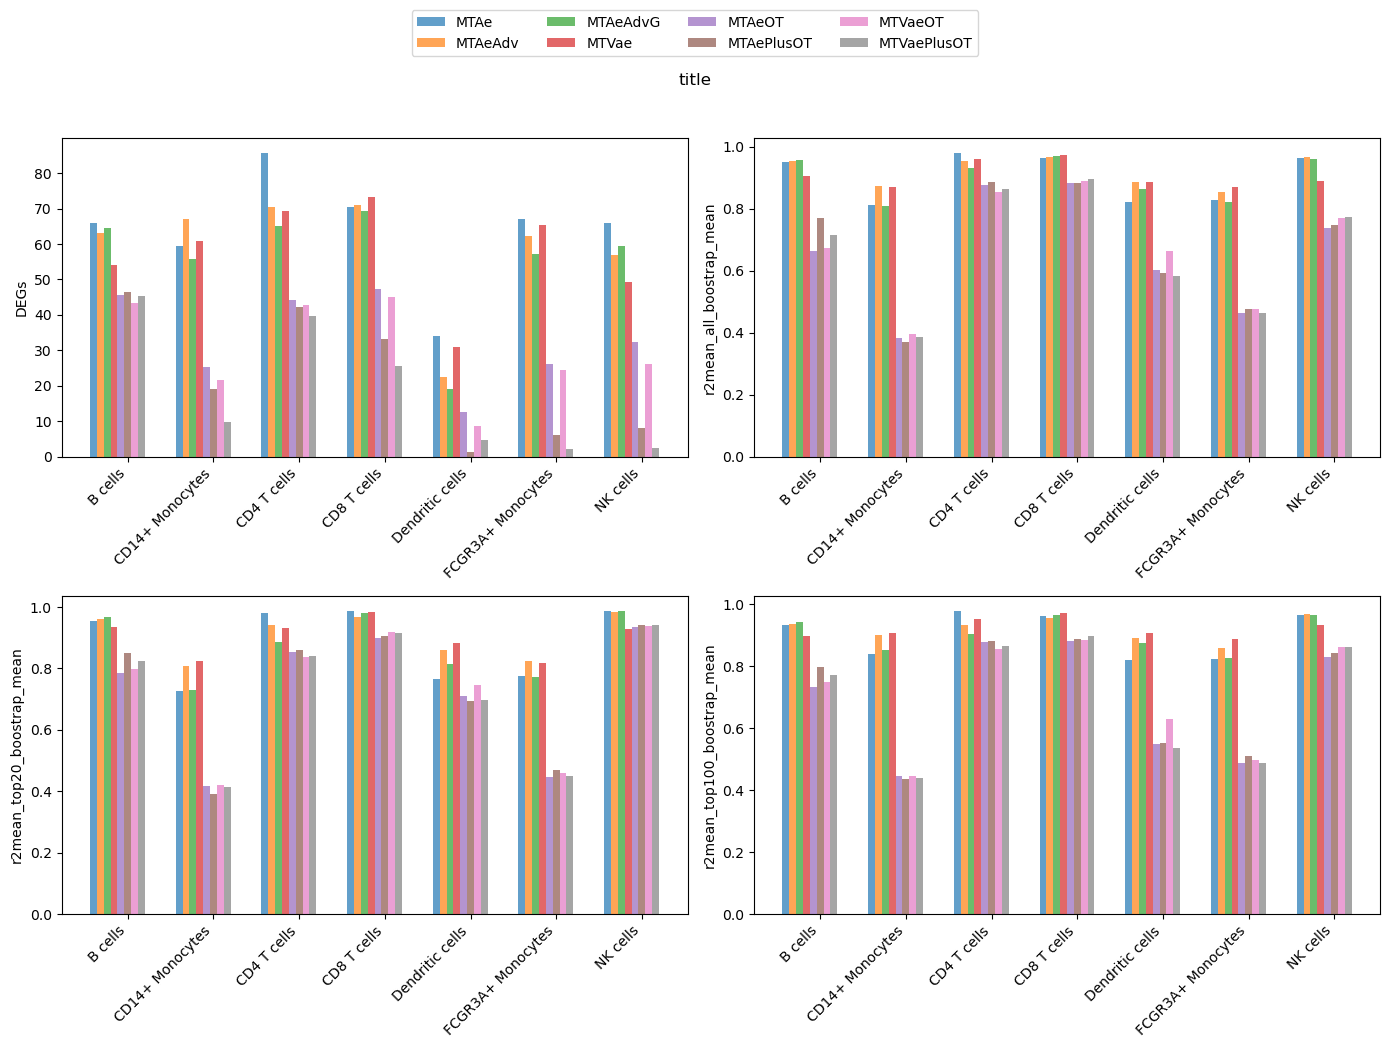
\includegraphics[width=.85\textwidth]{multi_task_benchmarking_cell_type_baseline_metrics_cross_study.png}
    \caption{Baseline metrics of multi-task models for the cross-study}
\end{figure}

\begin{figure}[h!]
    \centering
    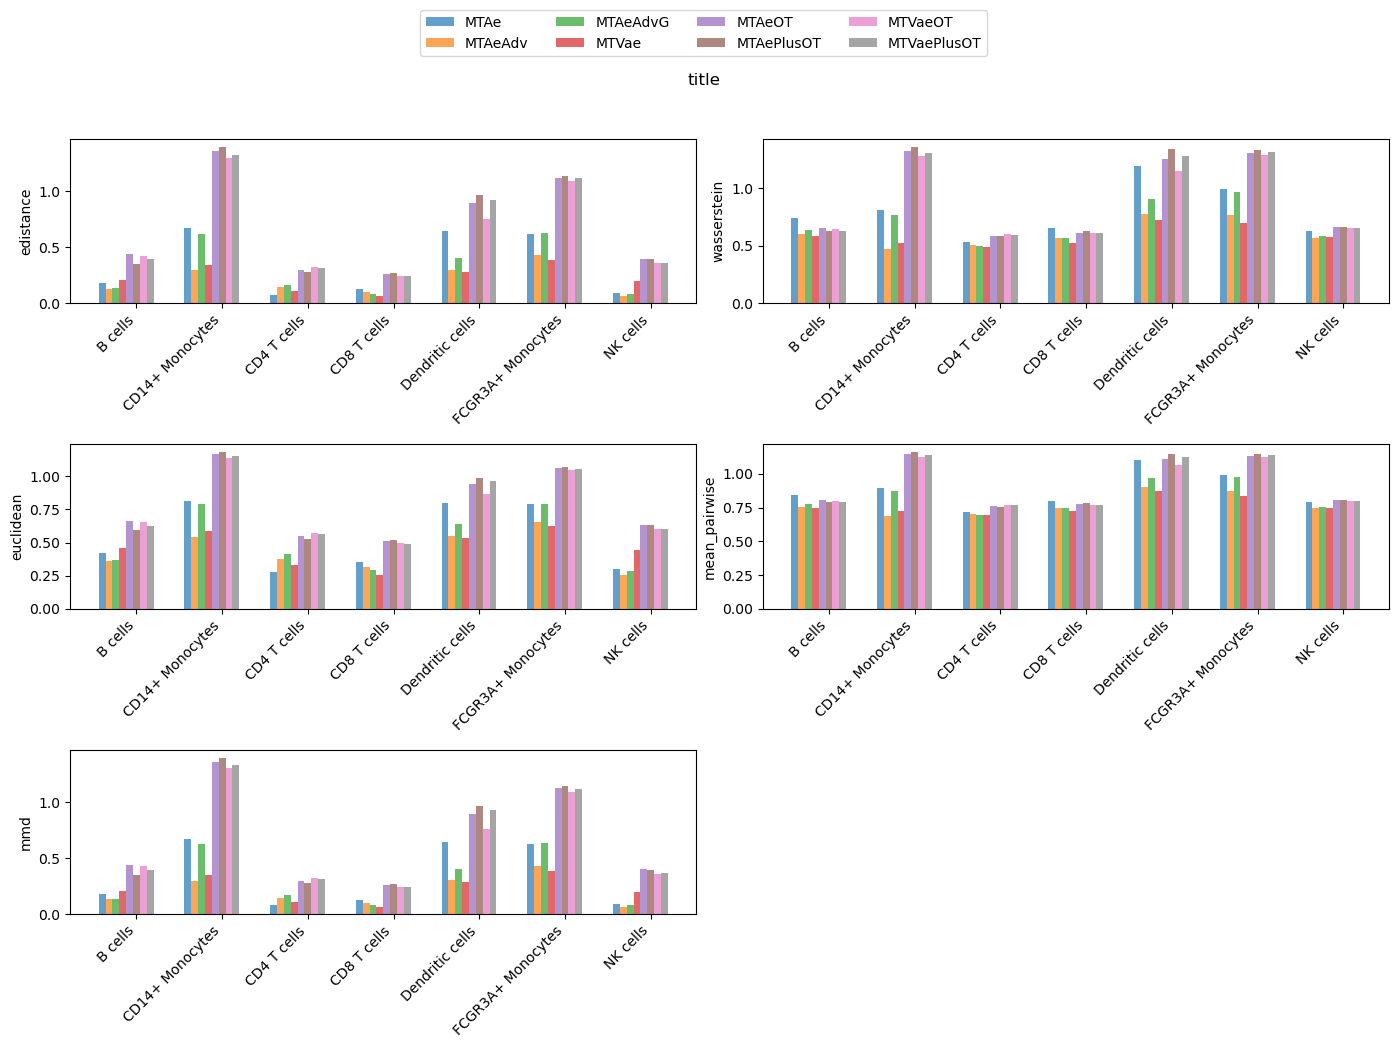
\includegraphics[width=.85\textwidth]{multi_task_benchmarking_cell_type_distance_metrics_cross_study.png}
    \caption{Distance metrics of multi-task models for the cross-study}
\end{figure}

\begin{figure}[h!]
    \centering
    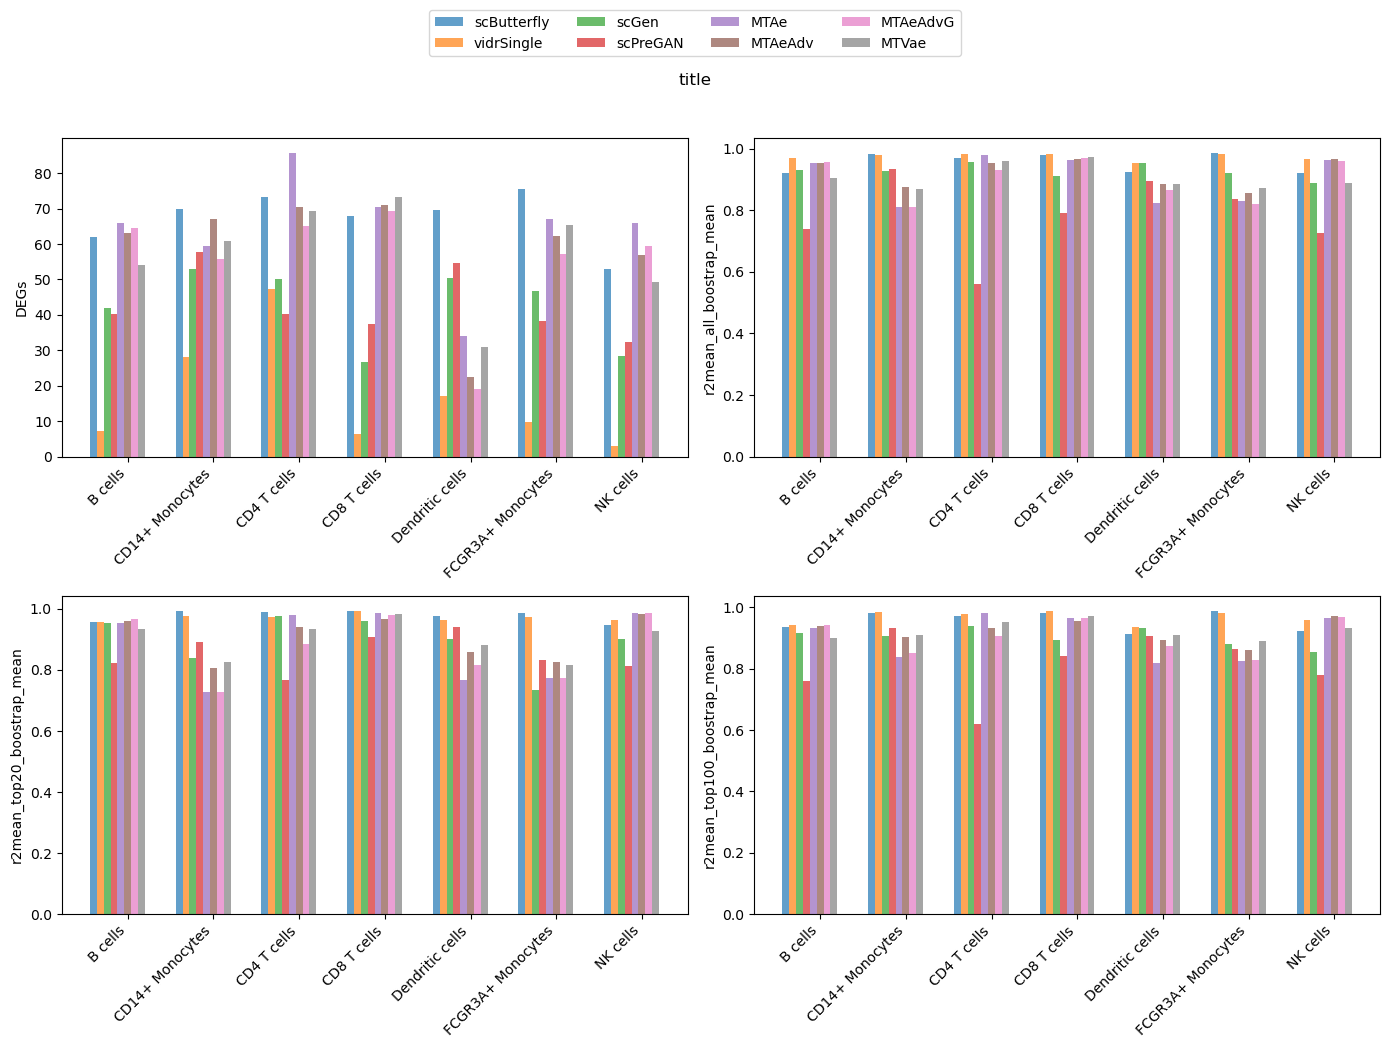
\includegraphics[width=.85\textwidth]{selected_benchmarking_cell_type_baseline_metrics_cross_study.png}
    \caption{Baseline metrics of multi-task and literature models for the cross-study}
    \label{}
\end{figure}

\begin{figure}[h!]
    \centering
    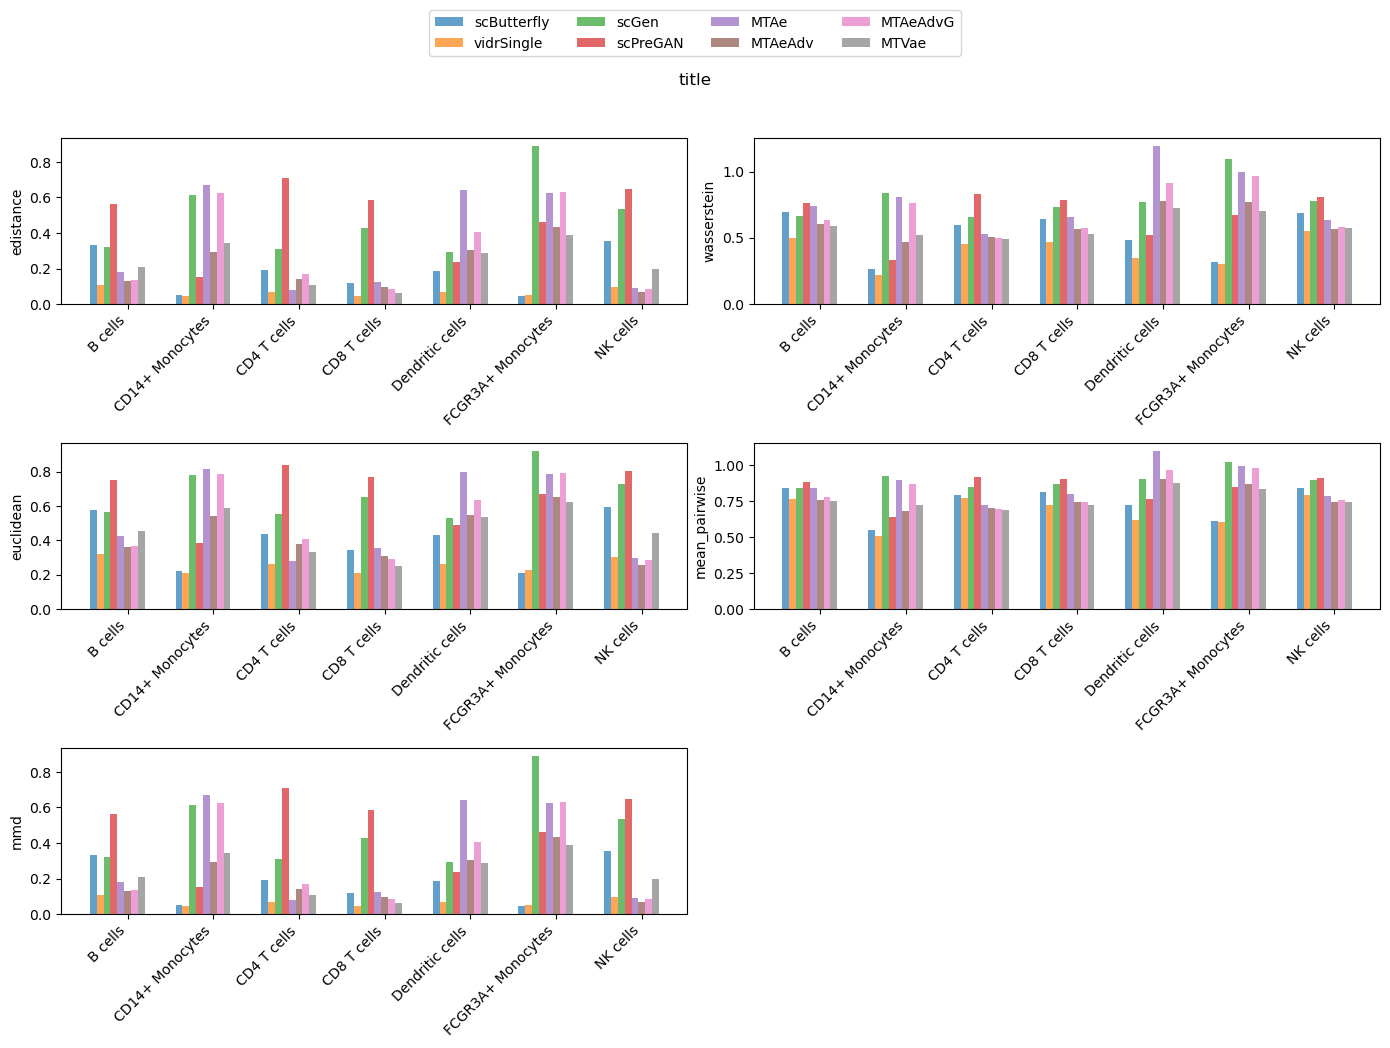
\includegraphics[width=.85\textwidth]{selected_benchmarking_cell_type_distance_metrics_cross_study.png}
    \caption{Distance metrics of multi-task and literature models for the cross-study}
    \label{}
\end{figure}

\begin{figure}[h!]
    \centering
    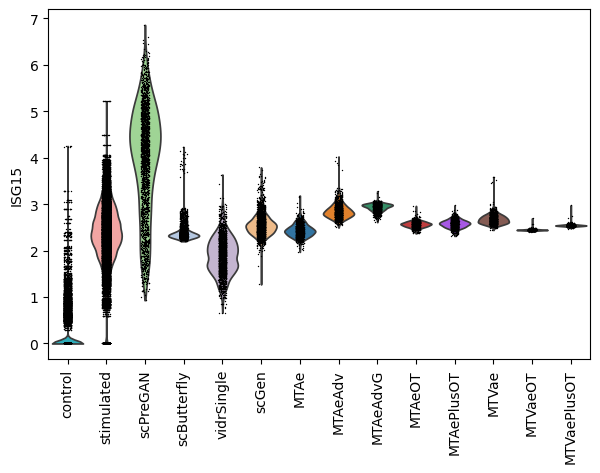
\includegraphics[width=.85\textwidth]{violins_cross_study.png}
    \caption{}
    \label{}
\end{figure}

\clearpage

\subsection{Cross-species}

\begin{table}[h!]
    \centering    
    \scalebox{0.8}{
    \begin{tabularx}{\textwidth}{lXXXXXXXXX}
    \toprule
    model & DEGs & $R^2_{\text{HVG}}$ & $R^2_{\text{HVG20}}$ & $R^2_{\text{HVG100}}$ & Euc & Was & E-dist & MPD & MMD \\
    \midrule
    MTAe & 0.000 (16.083) & 0.316 (0.740) & 0.451 (0.559) & 0.519 (0.481) & 0.036 (0.930) & 0.104 (1.008) & 0.055 (0.962) & 0.161 (0.995) & 0.036 (0.930) \\
    MTAeAdv & 0.547 (11.250) & 0.686 (0.579) & 0.731 (0.465) & 0.790 (0.365) & 0.010 (0.865) & 0.015 (0.919) & 0.016 (0.929) & 0.020 (0.957) & 0.010 (0.865) \\
    MTAeAdvG & 0.406 (12.500) & 0.391 (0.708) & 0.528 (0.533) & 0.577 (0.456) & 0.032 (0.921) & 0.082 (0.985) & 0.049 (0.958) & 0.132 (0.987) & 0.032 (0.921) \\
    MTAeOT & 0.972 (7.500) & 0.908 (0.483) & 0.827 (0.432) & 0.934 (0.304) & 0.023 (0.899) & 0.029 (0.932) & 0.038 (0.948) & 0.053 (0.966) & 0.023 (0.899) \\
    MTAePlusOT & 0.915 (8.000) & 0.915 (0.480) & 0.815 (0.436) & 0.923 (0.309) & 0.014 (0.876) & 0.010 (0.913) & 0.023 (0.936) & 0.017 (0.956) & 0.014 (0.876) \\
    MTVae & 0.406 (12.500) & 0.518 (0.652) & 0.631 (0.498) & 0.677 (0.413) & 0.000 (0.840) & 0.000 (0.903) & 0.000 (0.916) & 0.000 (0.951) & 0.000 (0.840) \\
    MTVaeOT & 0.981 (7.417) & 0.917 (0.479) & 0.855 (0.423) & 0.940 (0.302) & 0.022 (0.895) & 0.026 (0.929) & 0.035 (0.946) & 0.046 (0.964) & 0.022 (0.895) \\
    MTVaePlusOT & 0.934 (7.833) & 0.932 (0.473) & 0.830 (0.431) & 0.942 (0.301) & 0.017 (0.883) & 0.016 (0.919) & 0.028 (0.940) & 0.028 (0.959) & 0.017 (0.883) \\
    scButterfly & 0.604 (10.750) & 0.700 (0.574) & 0.956 (0.389) & 0.835 (0.346) & 0.023 (0.899) & 0.039 (0.942) & 0.038 (0.948) & 0.074 (0.971) & 0.023 (0.899) \\
    scGen & 0.962 (7.583) & 0.118 (0.826) & 0.016 (0.705) & 0.100 (0.658) & 0.461 (2.014) & 0.672 (1.576) & 0.529 (1.367) & 0.779 (1.165) & 0.461 (2.014) \\
    scPreGAN & 1.000 (7.250) & 1.000 (0.443) & 1.000 (0.374) & 1.000 (0.276) & 0.029 (0.914) & 0.042 (0.945) & 0.047 (0.955) & 0.079 (0.973) & 0.029 (0.914) \\
    vidrSingle & 0.358 (12.917) & 0.000 (0.878) & 0.000 (0.711) & 0.000 (0.701) & 1.000 (3.386) & 1.000 (1.905) & 1.000 (1.769) & 1.000 (1.225) & 1.000 (3.386) \\
    \bottomrule
    \end{tabularx}}
    \caption{Cross-species}
\end{table}

\begin{table}[h!]
    \centering    
    \scalebox{0.8}{    
    \begin{tabular}{lrrr}
    \toprule
    model & score & baseline score & distance score \\
    \midrule
    MTAe & 1.676506 & 1.285196 & 0.391310 \\
    MTAeAdvG & 2.227590 & 1.901575 & 0.326015 \\
    MTVae & 2.232088 & 2.232088 & 0.000000 \\
    MTAeAdv & 2.826189 & 2.754406 & 0.071783 \\
    scButterfly & 3.291590 & 3.094464 & 0.197126 \\
    MTAePlusOT & 3.646820 & 3.568396 & 0.078425 \\
    MTVaePlusOT & 3.743715 & 3.637807 & 0.105908 \\
    MTAeOT & 3.806643 & 3.640329 & 0.166315 \\
    MTVaeOT & 3.845143 & 3.693929 & 0.151214 \\
    scGen & 4.098110 & 1.196070 & 2.902040 \\
    scPreGAN & 4.225735 & 4.000000 & 0.225735 \\
    vidrSingle & 5.358491 & 0.358491 & 5.000000 \\
    \bottomrule
    \end{tabular}}
    \caption{Score Cross-Species}
\end{table}

\begin{figure}[h!]
    \centering
    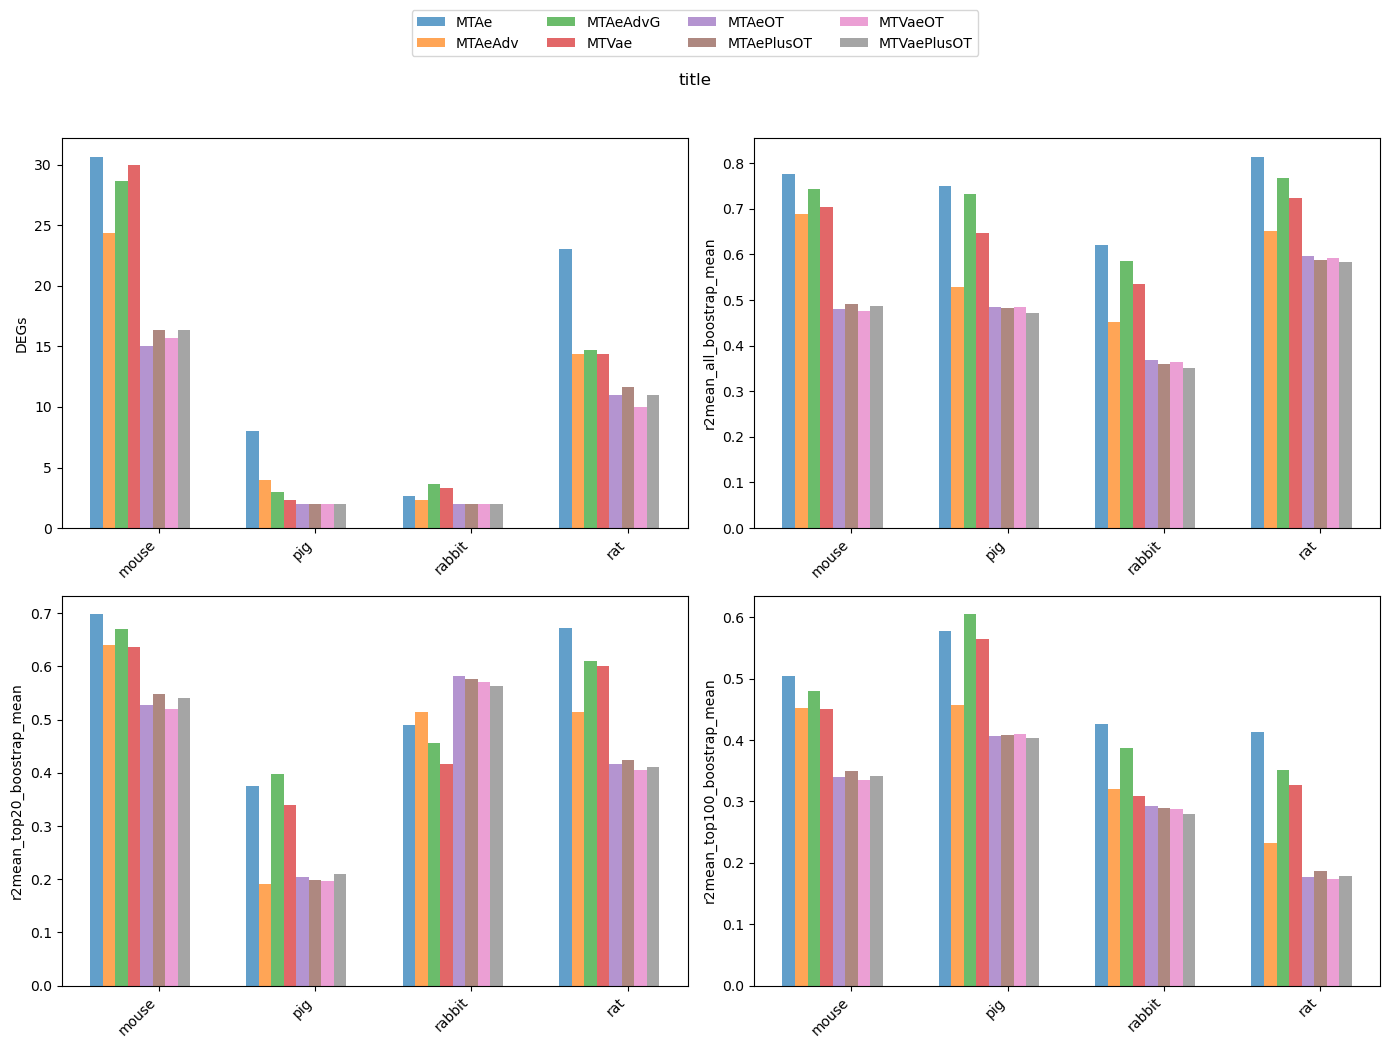
\includegraphics[width=.85\textwidth]{multi_task_benchmarking_cell_type_baseline_metrics_cross_species.png}
    \caption{Baseline metrics of multi-task models for the cross-species}
\end{figure}

\begin{figure}[h!]
    \centering
    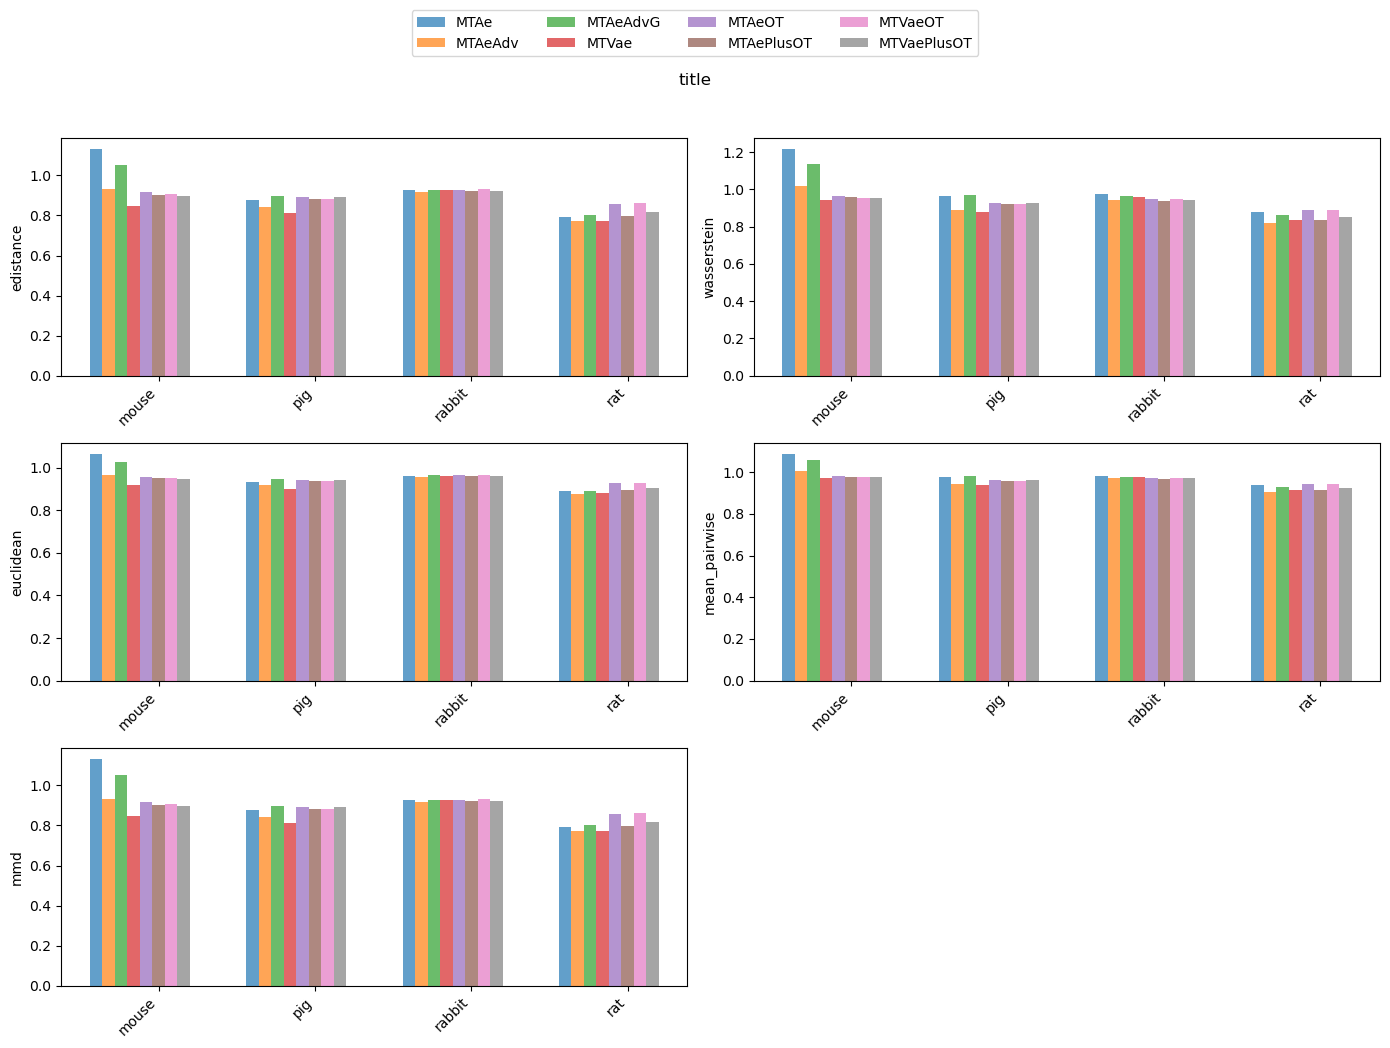
\includegraphics[width=.85\textwidth]{multi_task_benchmarking_cell_type_distance_metrics_cross_species.png}
    \caption{Distance metrics of multi-task models for the cross-species}
\end{figure}

\begin{figure}[h!]
    \centering
    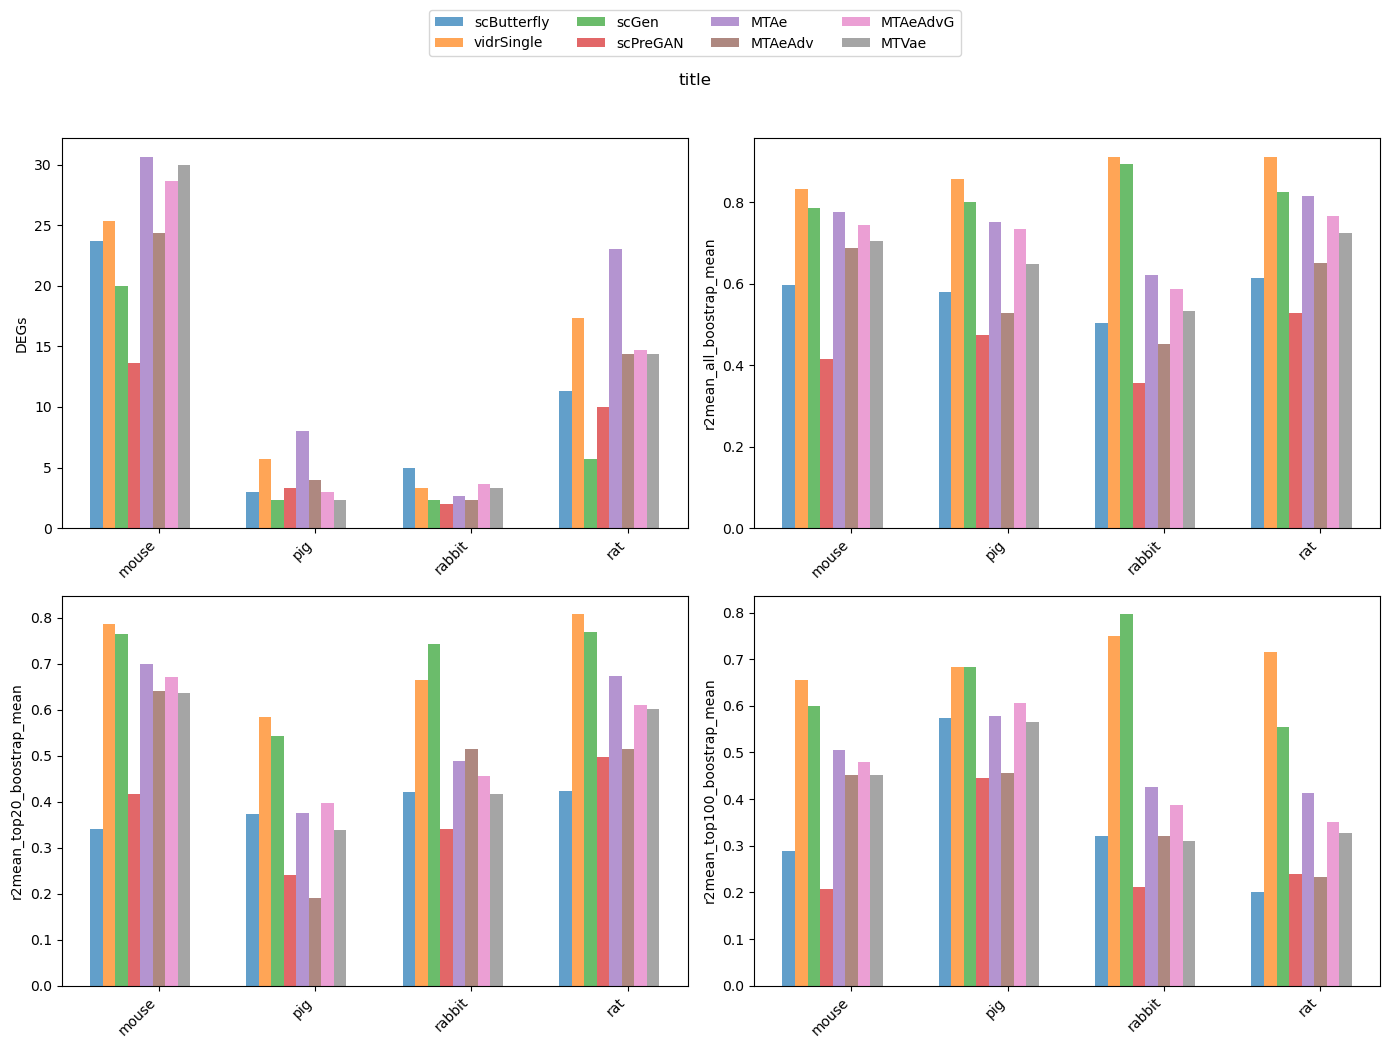
\includegraphics[width=.85\textwidth]{selected_benchmarking_cell_type_baseline_metrics_cross_species.png}
    \caption{Baseline metrics of multi-task and literature models for the cross-species}
    \label{}
\end{figure}

\begin{figure}[h!]
    \centering
    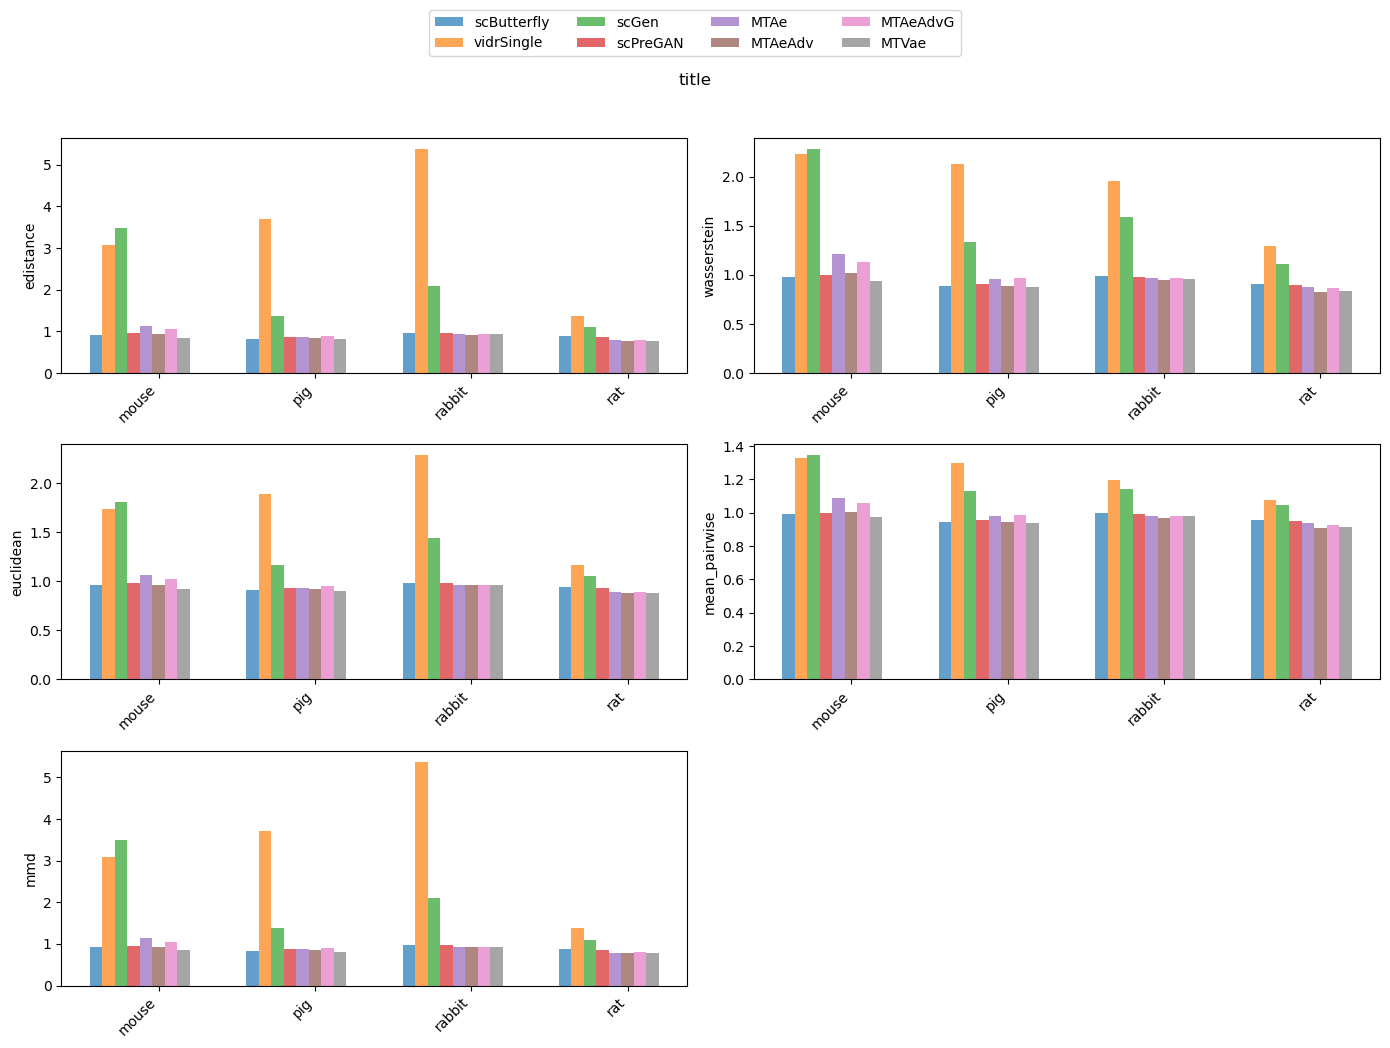
\includegraphics[width=.85\textwidth]{selected_benchmarking_cell_type_distance_metrics_cross_species.png}
    \caption{Distance metrics of multi-task and literature models for the cross-species}
    \label{}
\end{figure}

\begin{figure}[h!]
    \centering
    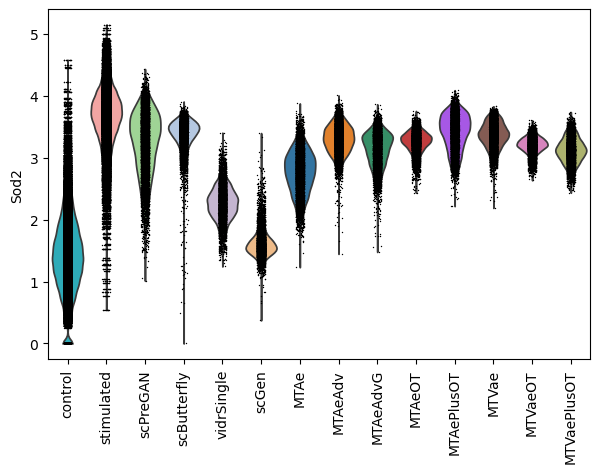
\includegraphics[width=.85\textwidth]{violins_cross_species.png}
    \caption{}
    \label{}
\end{figure}


\clearpage

\subsection{Nault et al.}
    

\begin{table}[h!]
    \centering
    \scalebox{0.8}{
    \begin{tabularx}{\textwidth}{lXXXXXXXXX}
    \toprule
    model & DEGs & $R^2_{\text{HVG}}$ & $R^2_{\text{HVG20}}$ & $R^2_{\text{HVG100}}$ & Euc & Was & E-dist & MPD & MMD \\
    \midrule
    MTAe & \textbf{0.000 (20.341)} & 0.167 (0.862) & 0.267 (0.792) & 0.189 (0.833) & 0.056 (1.386) & 0.603 (1.217) & 0.116 (1.116) & 0.945 (1.050) & 0.056 (1.386) \\
    MTAeAdv & 0.368 (13.716) & 0.388 (0.792) & 0.518 (0.725) & 0.458 (0.743) & 0.025 (1.128) & 0.246 (1.091) & 0.045 (1.011) & 0.426 (1.017) & 0.025 (1.128) \\
    MTAeAdvG & 0.113 (18.307) & 0.339 (0.808) & 0.477 (0.736) & 0.396 (0.764) & 0.029 (1.164) & 0.293 (1.107) & 0.058 (1.030) & 0.607 (1.029) & 0.029 (1.164) \\
    MTAeOT & 0.650 (8.652) & 0.969 (0.608) & 0.829 (0.642) & 0.916 (0.590) & 0.001 (0.925) & 0.008 (1.006) & 0.005 (0.951) & 0.122 (0.998) & 0.001 (0.925) \\
    MTAePlusOT & 0.657 (8.519) & 0.956 (0.613) & 0.822 (0.644) & 0.897 (0.596) & \textbf{0.000 (0.917)} & \textbf{0.000 (1.004)} & 0.002 (0.948) & 0.099 (0.996) & 0.000 (0917) \\
    MTVae & 0.076 (18.981) & 0.339 (0.808) & 0.523 (0.724) & 0.428 (0.753) & 0.025 (1.124) & 0.273 (1.100) & 0.041 (1.005) & 0.413 (1.016) & 0.025 (1.124) \\
    MTVaeOT & 0.677 (8.163) & 0.953 (0.614) & 0.830 (0.642) & 0.906 (0.593) & 0.001 (0.929) & 0.016 (1.009) & 0.006 (0.952) & 0.132 (0.998) & 0.001 (0.929) \\
    MTVaePlusOT & 0.647 (8.701) & 0.948 (0.615) & 0.816 (0.645) & 0.894 (0.597) & 0.000 (0.919) & 0.008 (1.006) & 0.003 (0.948) & 0.112 (0.997) & \textbf{0.000 (0.919)} \\
    scButterfly & 0.196 (16.818) & 0.553 (0.740) & 0.633 (0.694) & 0.600 (0.696) & 0.008 (0.984) & 0.029 (1.014) & \textbf{0.000 (0.944)} & \textbf{0.000 (0.990)} & 0.008 (0.984) \\
    scGen & 0.781 (6.288) & \textbf{0.000 (0.915)} & \textbf{0.000 (0.863)} & \textbf{0.000 (0.897)} & 0.178 (2.408) & 0.637 (1.229) & 0.299 (1.387) & 0.805 (1.041) & 0.178 (2.408) \\
    scPreGAN & 0.324 (14.511) & 1.000 (0.599) & 1.000 (0.596) & 1.000 (0.562) & 0.007 (0.972) & 0.042 (1.019) & 0.017 (0.969) & 0.163 (1.000) & 0.007 (0.972) \\
    vidrMult & 1.000 (2.352) & 0.143 (0.870) & 0.099 (0.837) & 0.133 (0.852) & 1.000 (9.295) & 1.000 (1.358) & 1.000 (2.425) & 1.000 (1.054) & 1.000 (9.295) \\
    vidrSingle & 0.920 (3.795) & 0.191 (0.855) & 0.247 (0.797) & 0.216 (0.824) & 0.061 (1.431) & 0.480 (1.174) & 0.117 (1.118) & 0.544 (1.025) & 0.061 (1.431) \\
    \bottomrule
    \end{tabularx}}
    \caption{Score of the models for Nault et al. \cite{nault2021single,nault2022benchmarking} along with the actual value in parenthesis}
\end{table}

\begin{table}[h!]
    \centering
    \scalebox{0.8}{    
    \begin{tabular}{lrrr}
    \toprule
    model & score & baseline score & distance score \\
    \midrule
    scButterfly & 2.026767 & 1.981569 & 0.045198 \\
    MTVae & 2.142595 & 1.365570 & 0.777025 \\
    MTAeAdvG & 2.341641 & 1.324716 & 1.016925 \\
    MTAe & 2.398554 & 0.622043 & 1.776511 \\
    MTAeAdv & 2.498785 & 1.731406 & 0.767379 \\
    vidrSingle & 2.837696 & 1.573823 & 1.263873 \\
    scGen & 2.878990 & 0.781217 & 2.097772 \\
    MTVaePlusOT & 3.428329 & 3.305106 & 0.123224 \\
    MTAePlusOT & 3.433685 & 3.332175 & 0.101511 \\
    MTAeOT & 3.500992 & 3.363746 & 0.137247 \\
    MTVaeOT & 3.522593 & 3.365641 & 0.156953 \\
    scPreGAN & 3.559583 & 3.324068 & 0.235515 \\
    vidrMult & 6.375357 & 1.375357 & 5.000000 \\
    \bottomrule
    \end{tabular}
    }
    \caption{Nault et al. \cite{nault2021single,nault2022benchmarking}}
\end{table}



\begin{figure}[h!]
    \centering
    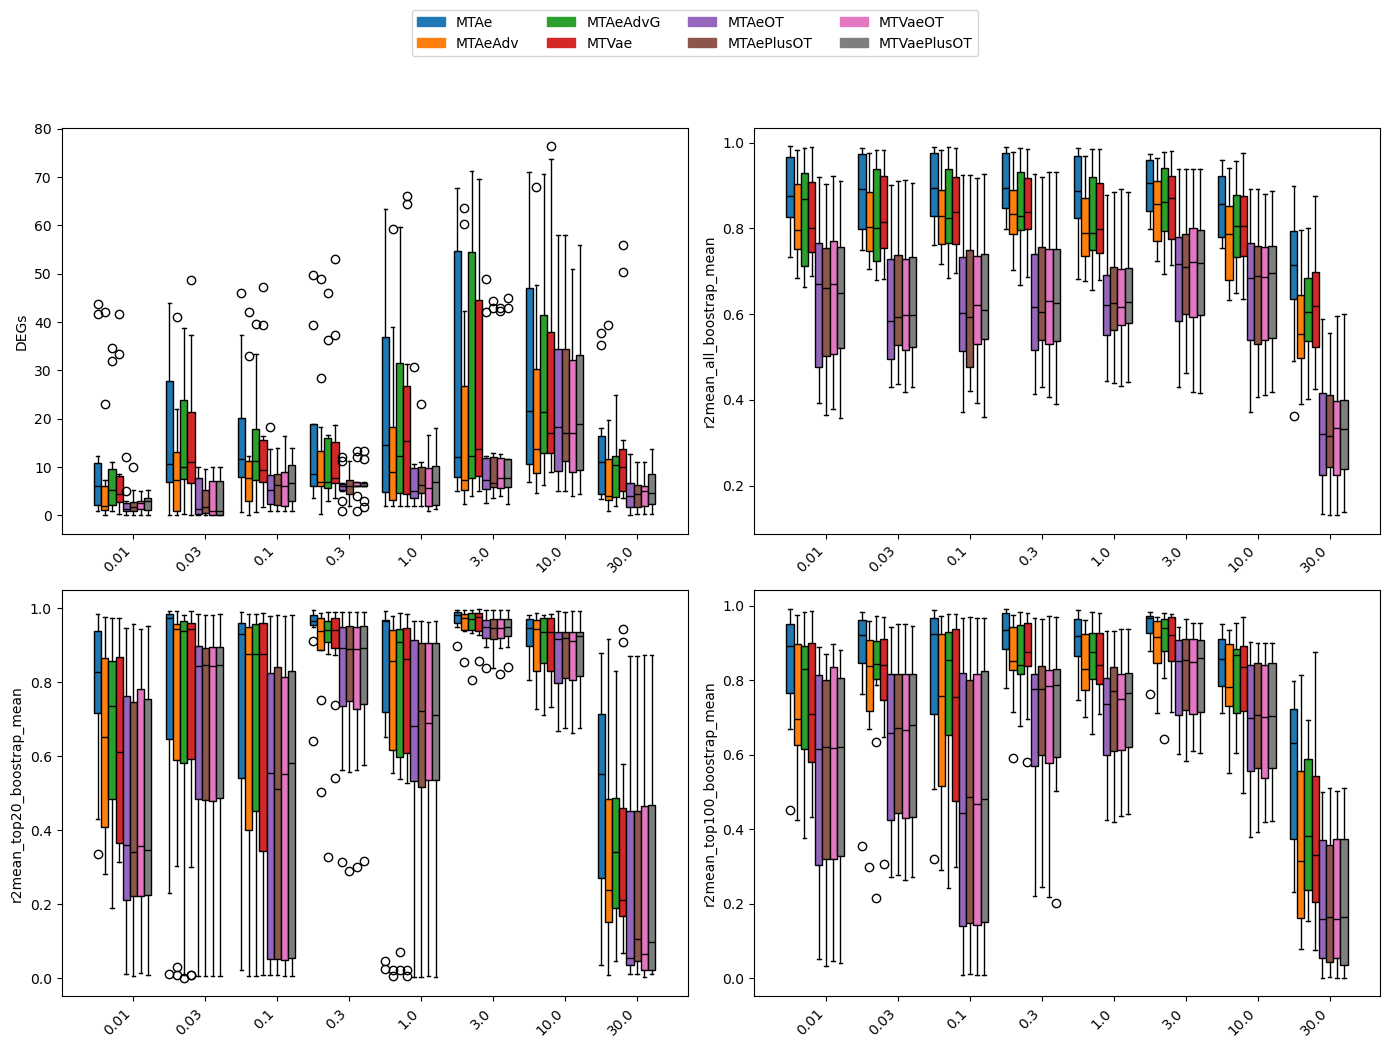
\includegraphics[width=.85\textwidth]{multi_task_benchmarking_doses_baseline_metrics_nault.png}
    \caption{Baseline metrics of multi-task models for the Nault et al. \cite{nault2021single,nault2022benchmarking} dataset across dosages}
\end{figure}

\begin{figure}[h!]
    \centering
    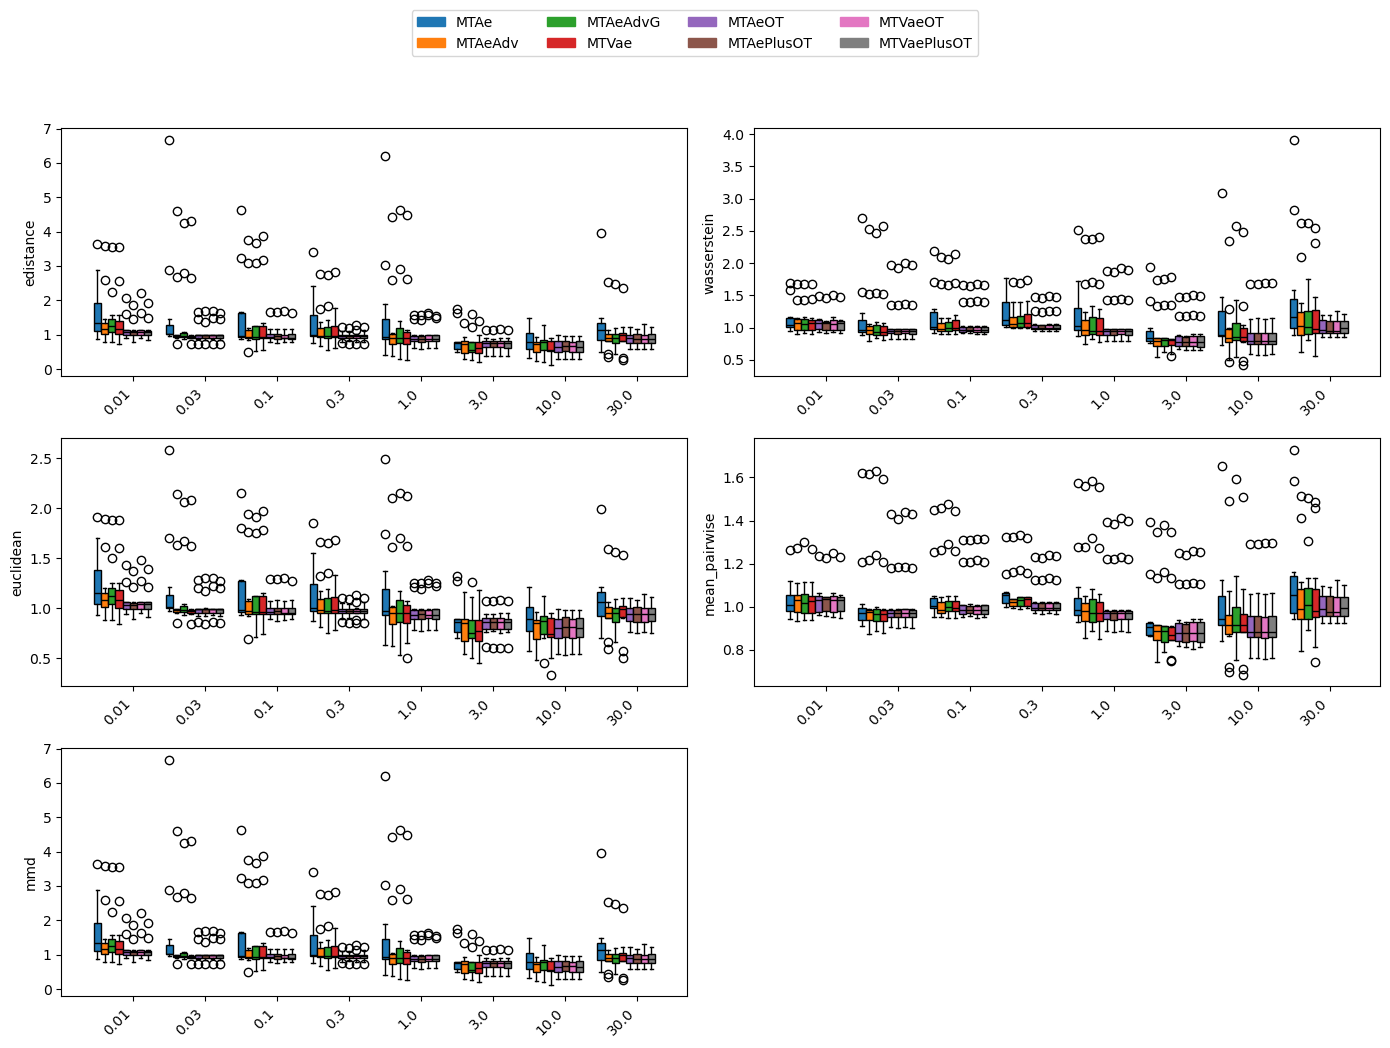
\includegraphics[width=.85\textwidth]{multi_task_benchmarking_doses_distance_metrics_nault.png}
    \caption{Distance metrics of multi-task models for the Nault et al. \cite{nault2021single,nault2022benchmarking} dataset across dosages}
\end{figure}


\begin{figure}[h!]
    \centering
    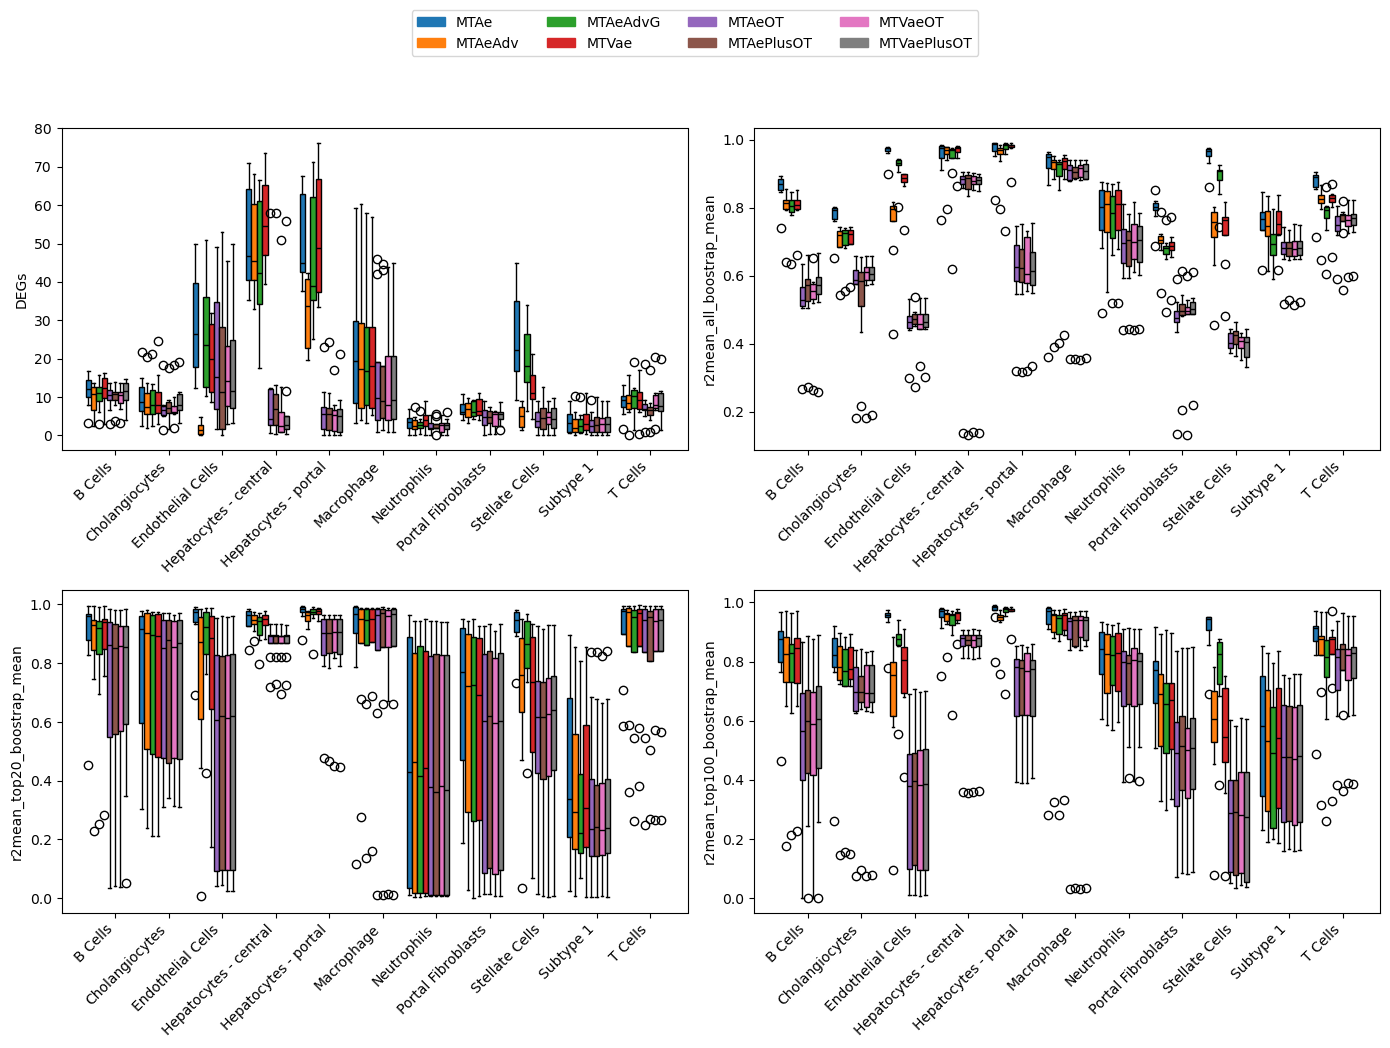
\includegraphics[width=.85\textwidth]{multi_task_benchmarking_cell_type_baseline_metrics_nault.png}
    \caption{Baseline metrics of multi-task models for the Nault et al. \cite{nault2021single,nault2022benchmarking} dataset across cell types}
\end{figure}


\begin{figure}[h!]
    \centering
    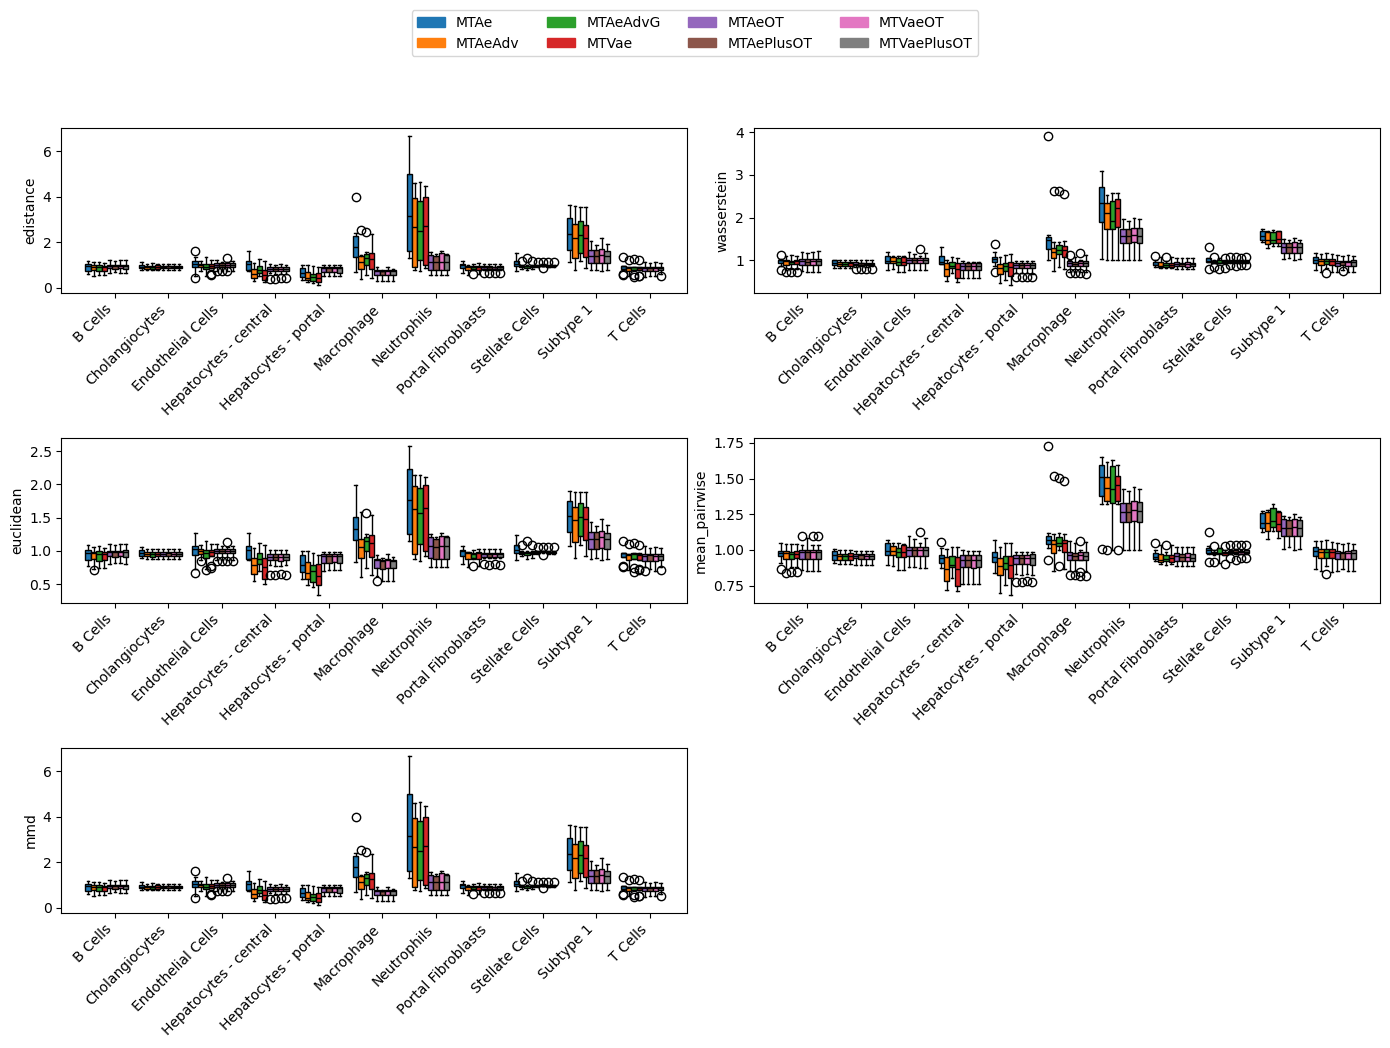
\includegraphics[width=.85\textwidth]{multi_task_benchmarking_cell_type_distance_metrics_nault.png}
    \caption{Distance metrics of multi-task models for the Nault et al. \cite{nault2021single,nault2022benchmarking} dataset across cell types}
\end{figure}


\begin{figure}[h!]
    \centering
    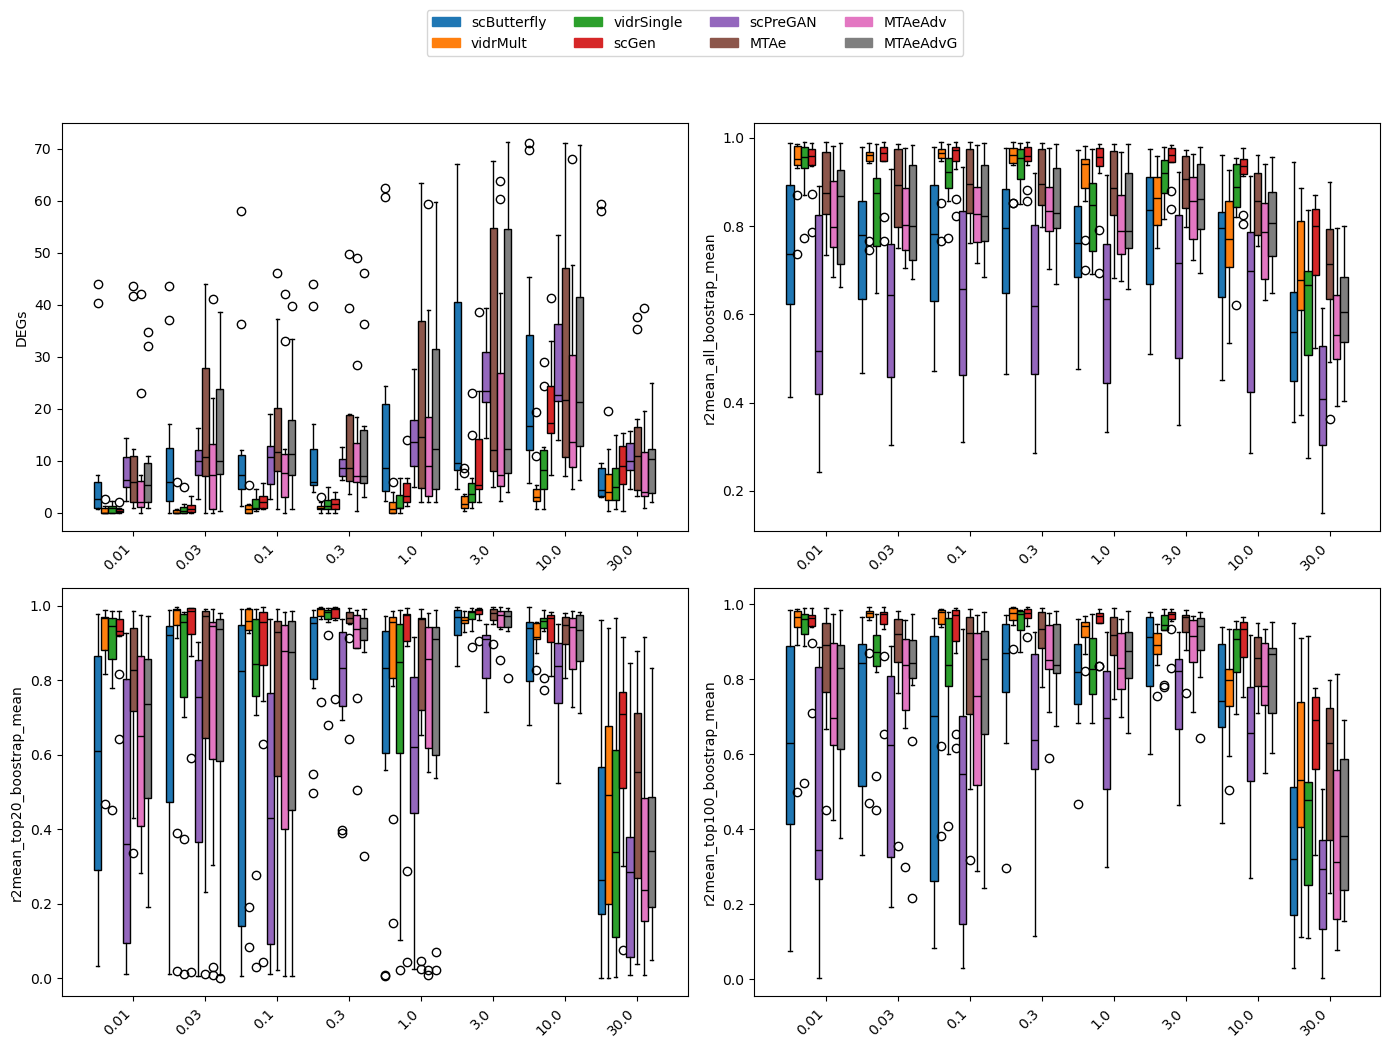
\includegraphics[width=.85\textwidth]{selected_benchmarking_doses_baseline_metrics_nault.png}
    \caption{Baseline metrics of multi-task and literature models for the Nault et al. \cite{nault2021single,nault2022benchmarking} dataset across dosages}
    \label{fig:selected_nault_doses_baseline}
\end{figure}

\begin{figure}[h!]
    \centering
    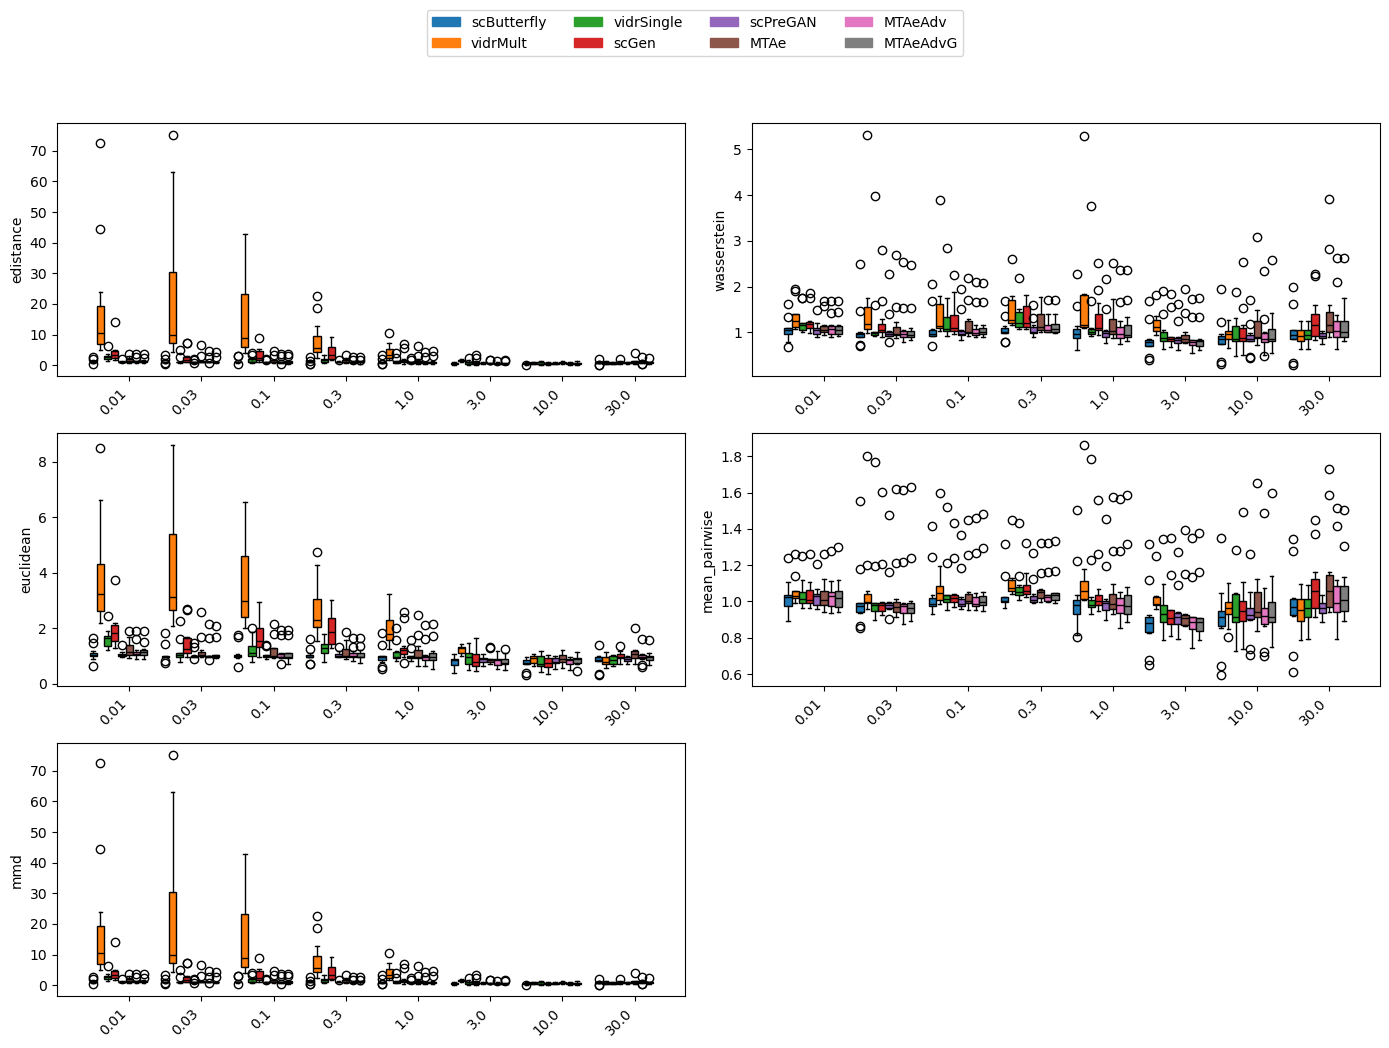
\includegraphics[width=.85\textwidth]{selected_benchmarking_doses_distance_metrics_nault.png}
    \caption{Distance metrics of multi-task and literature models for the Nault et al. \cite{nault2021single,nault2022benchmarking} dataset across dosages}
    \label{fig:selected_nault_doses_distance}
\end{figure}


\begin{figure}[h!]
    \centering
    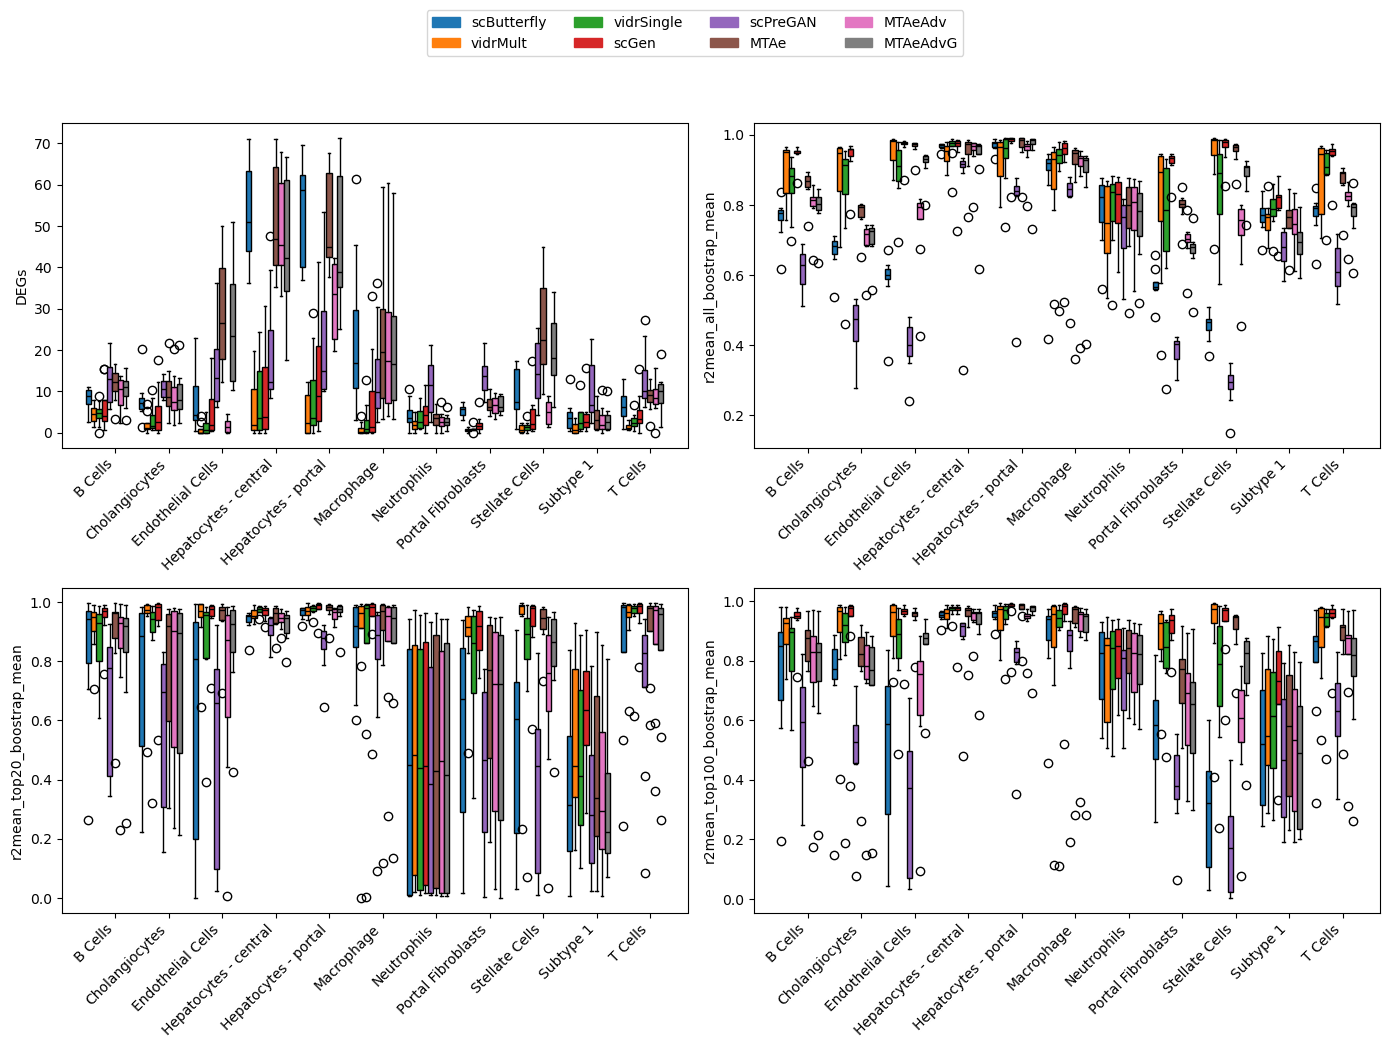
\includegraphics[width=.85\textwidth]{selected_benchmarking_cell_type_baseline_metrics_nault.png}
    \caption{Baseline metrics of multi-task and literature models for the Nault et al. \cite{nault2021single,nault2022benchmarking} dataset across cell types}
    \label{fig:selected_nault_cell_type_baseline}
\end{figure}


\begin{figure}[h!]
    \centering
    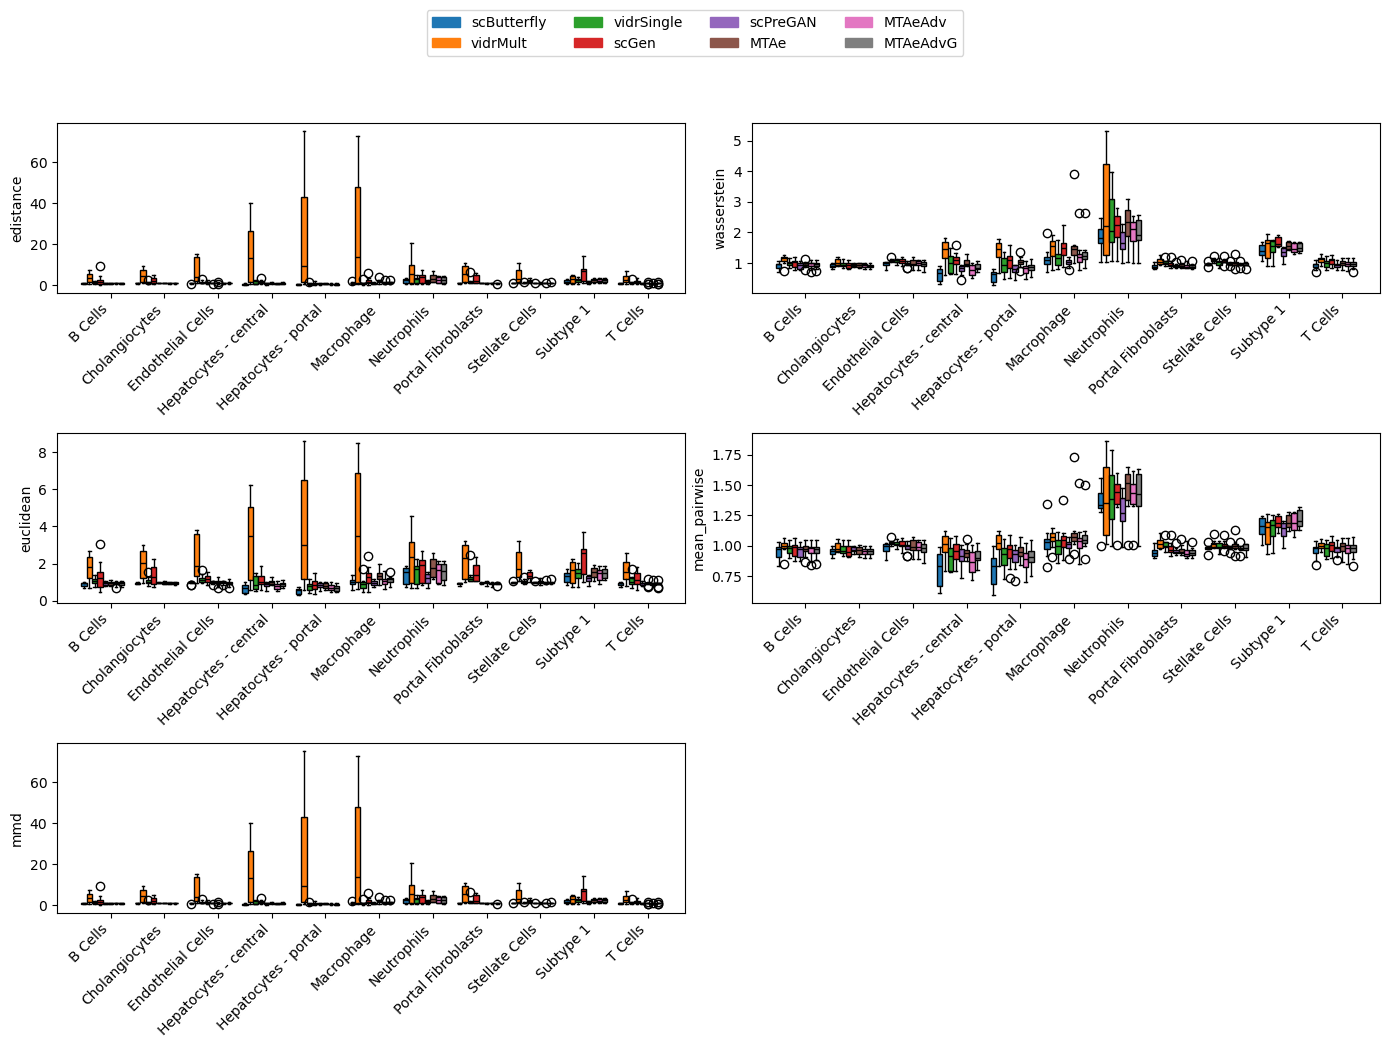
\includegraphics[width=.85\textwidth]{selected_benchmarking_cell_type_distance_metrics_nault.png}
    \caption{Distance metrics of multi-task and literature models for the Nault et al. \cite{nault2021single,nault2022benchmarking} dataset across cell types}
    \label{fig:selected_nault_cell_type_distance}
\end{figure}

% dotplots and latent umaps of the selected models comparison


\clearpage


\subsection{Knowledge transfer}

which tasks and why they are important?

\subsection{TODO}

\begin{itemize}
    \item interpretability
    \item explainability
    \item integration with multiple omics
\end{itemize}

\section{Interpretability}


\section{Conclusion and future work}

We have validated the potential of scButterfly to perturbation modeling with the multi-dosage dataset of Nault et al. \cite{nault2021single,nault2022benchmarking}, an addition of the author's study that is based only on the dataset of Kang et al. \cite{kanaGenerativeModelingSinglecell2023}. We have proposed multi-task architectures that can be used for perturbation modeling, and we have benchmarked them against the state-of-the-art models in the field. The results show that our models outperform or are comparable to the state-of-the-art models in the field.

Another significant benefit of our model is its lower complexity while scaling to a larger number of perturbations (scalability)\cite{allenspachNeuralMultitaskLearning2024}.

It should be noted that one of the limitations of our methods is the transductive learning with respect to the perturbations. The perturbation signal is one-hot encoded, thus limiting the model to generalize to unseen ones. Thus, future work could include to explore how inductive learning with respect to the perturbations could be integrated to our architecture, enabling extrapolation to unseen perturbations.

\section{Code availability}

The code for the models and the experiments is available at \url{https://github.com/thodkatz/thesis}.

\clearpage


%\chapter{Benchmarking}
\label{ch:chapter1}

\clearpage


\section{Datasets}

\subsection{Nault et al. 2022}

\begin{figure}[h]
    \centering
    \begin{subfigure}[t]{0.49\textwidth}
        \centering
        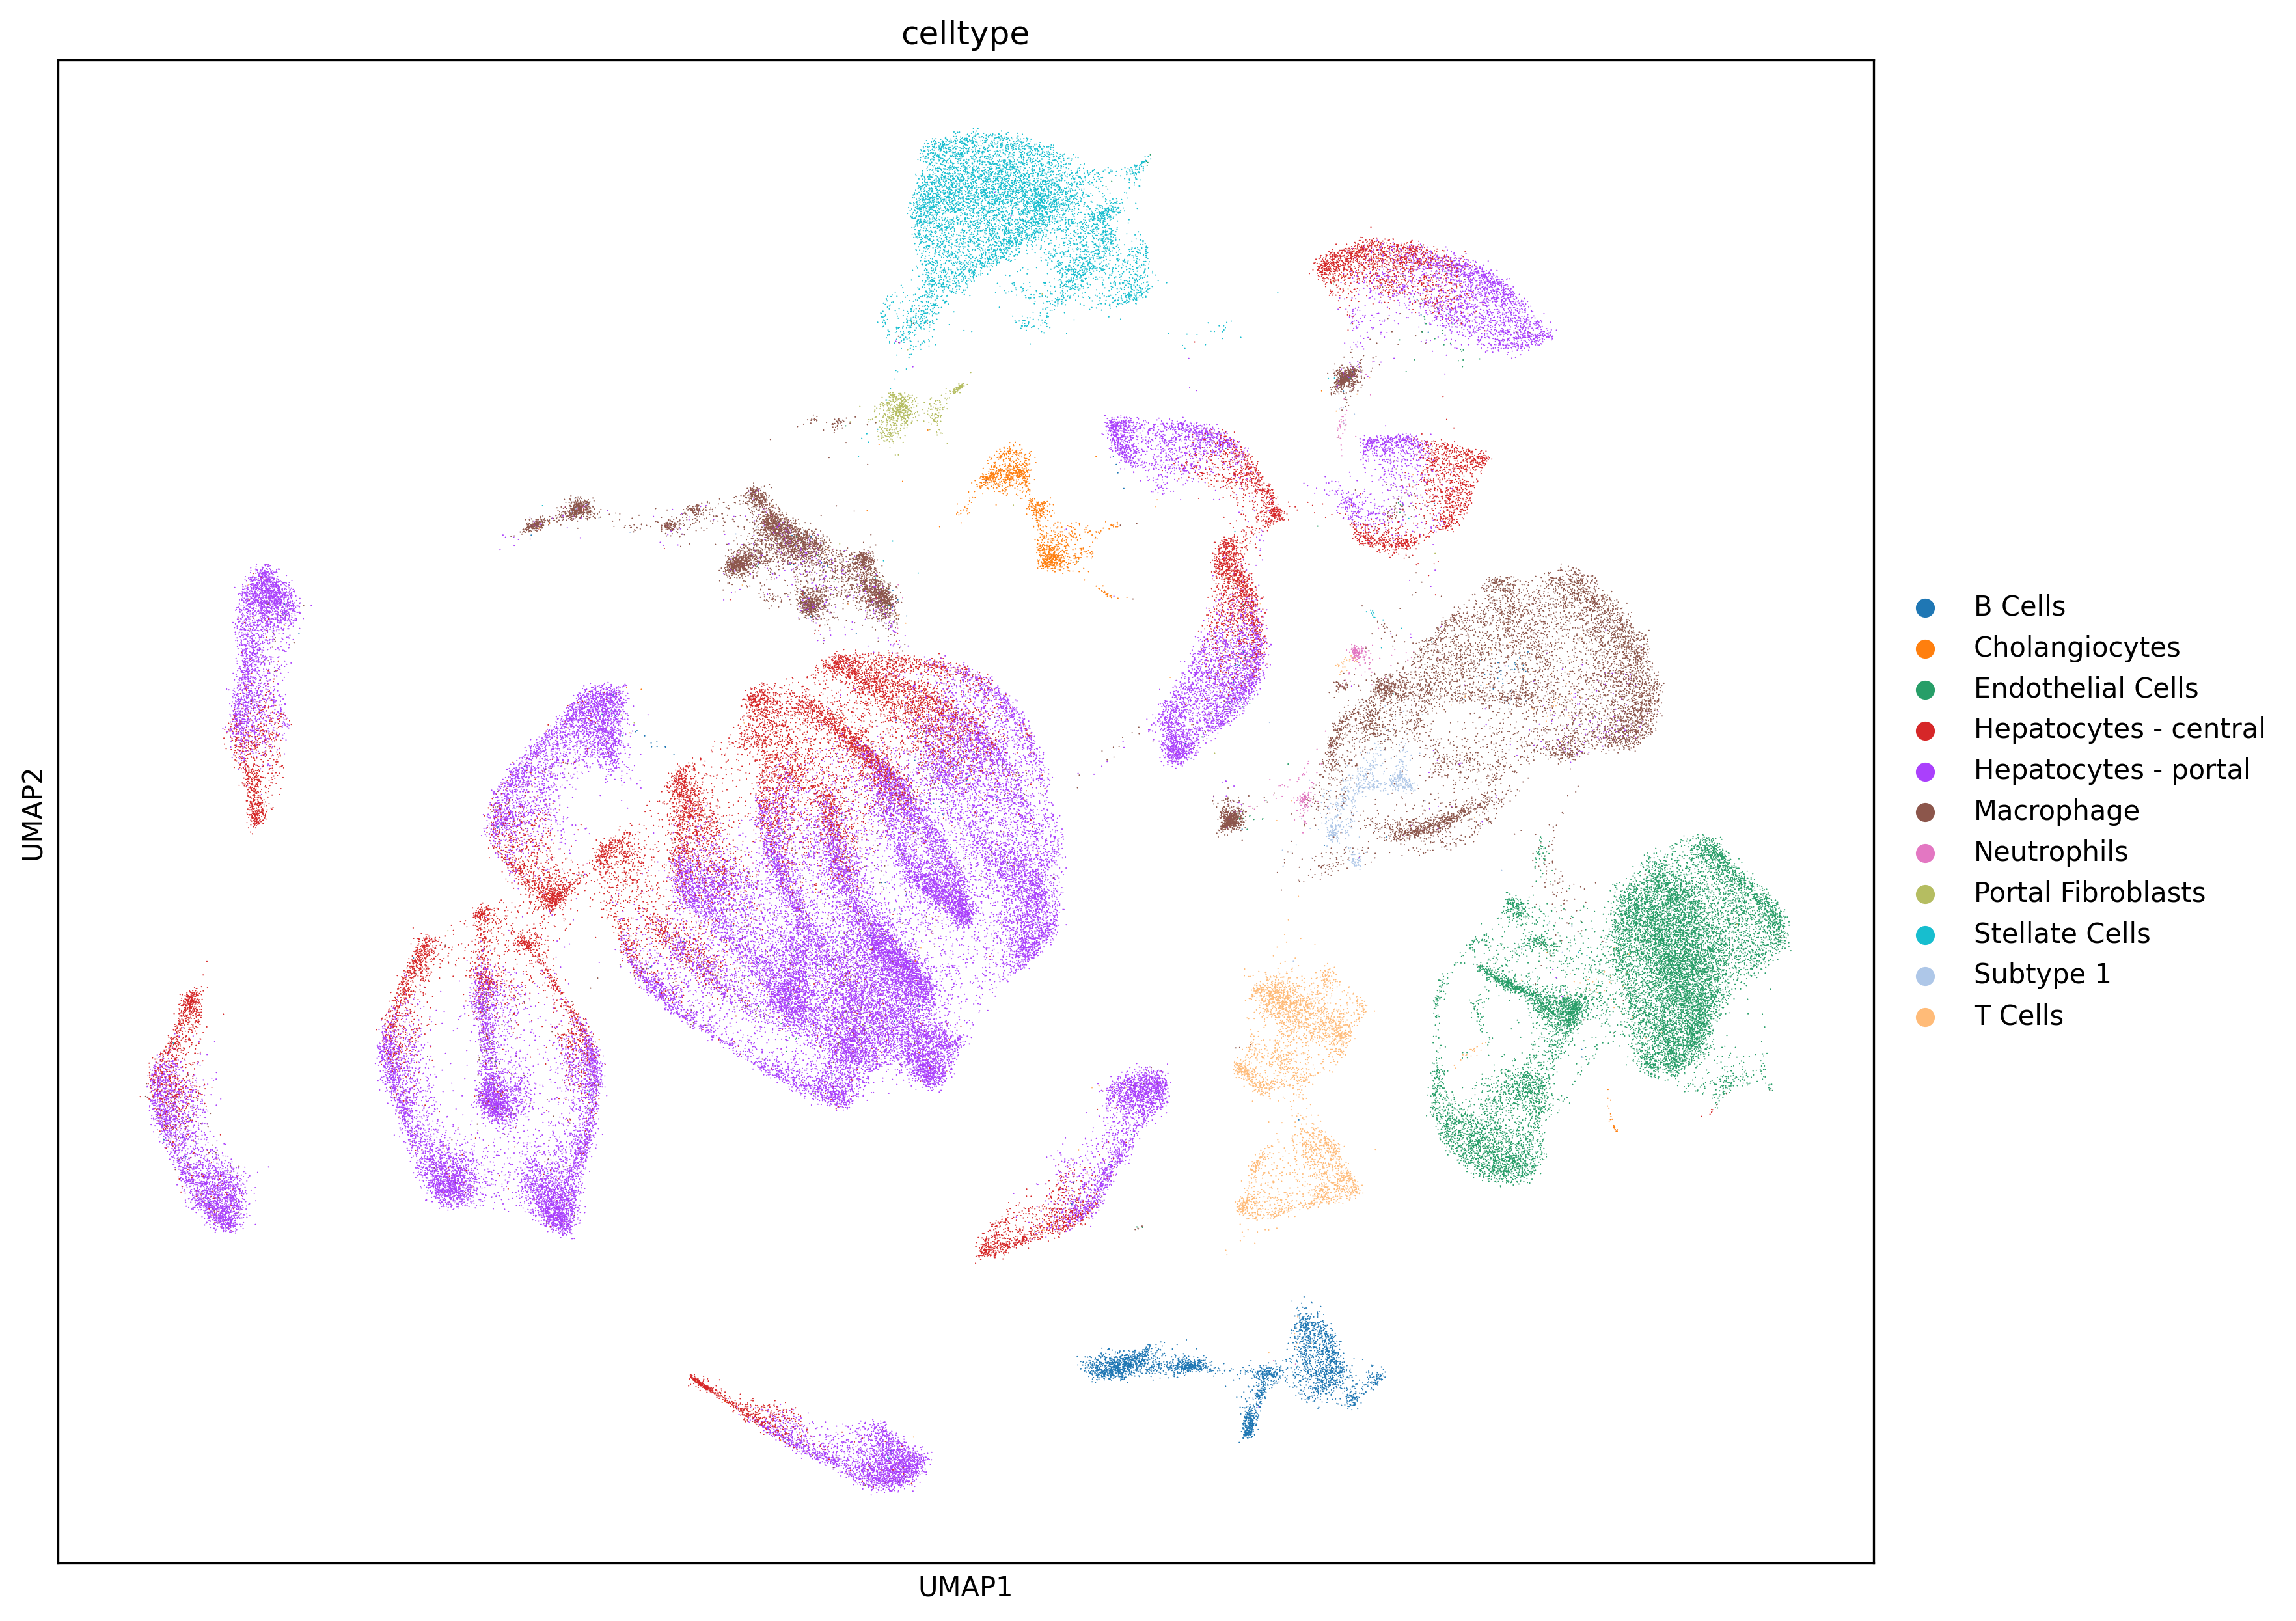
\includegraphics[width=.9\textwidth]{figures/nault_cell_umap.png}
        \caption{}
        \label{fig:figure1}.
    \end{subfigure}%
    \hfill
    \begin{subfigure}[t]{0.49\textwidth}
        \centering
        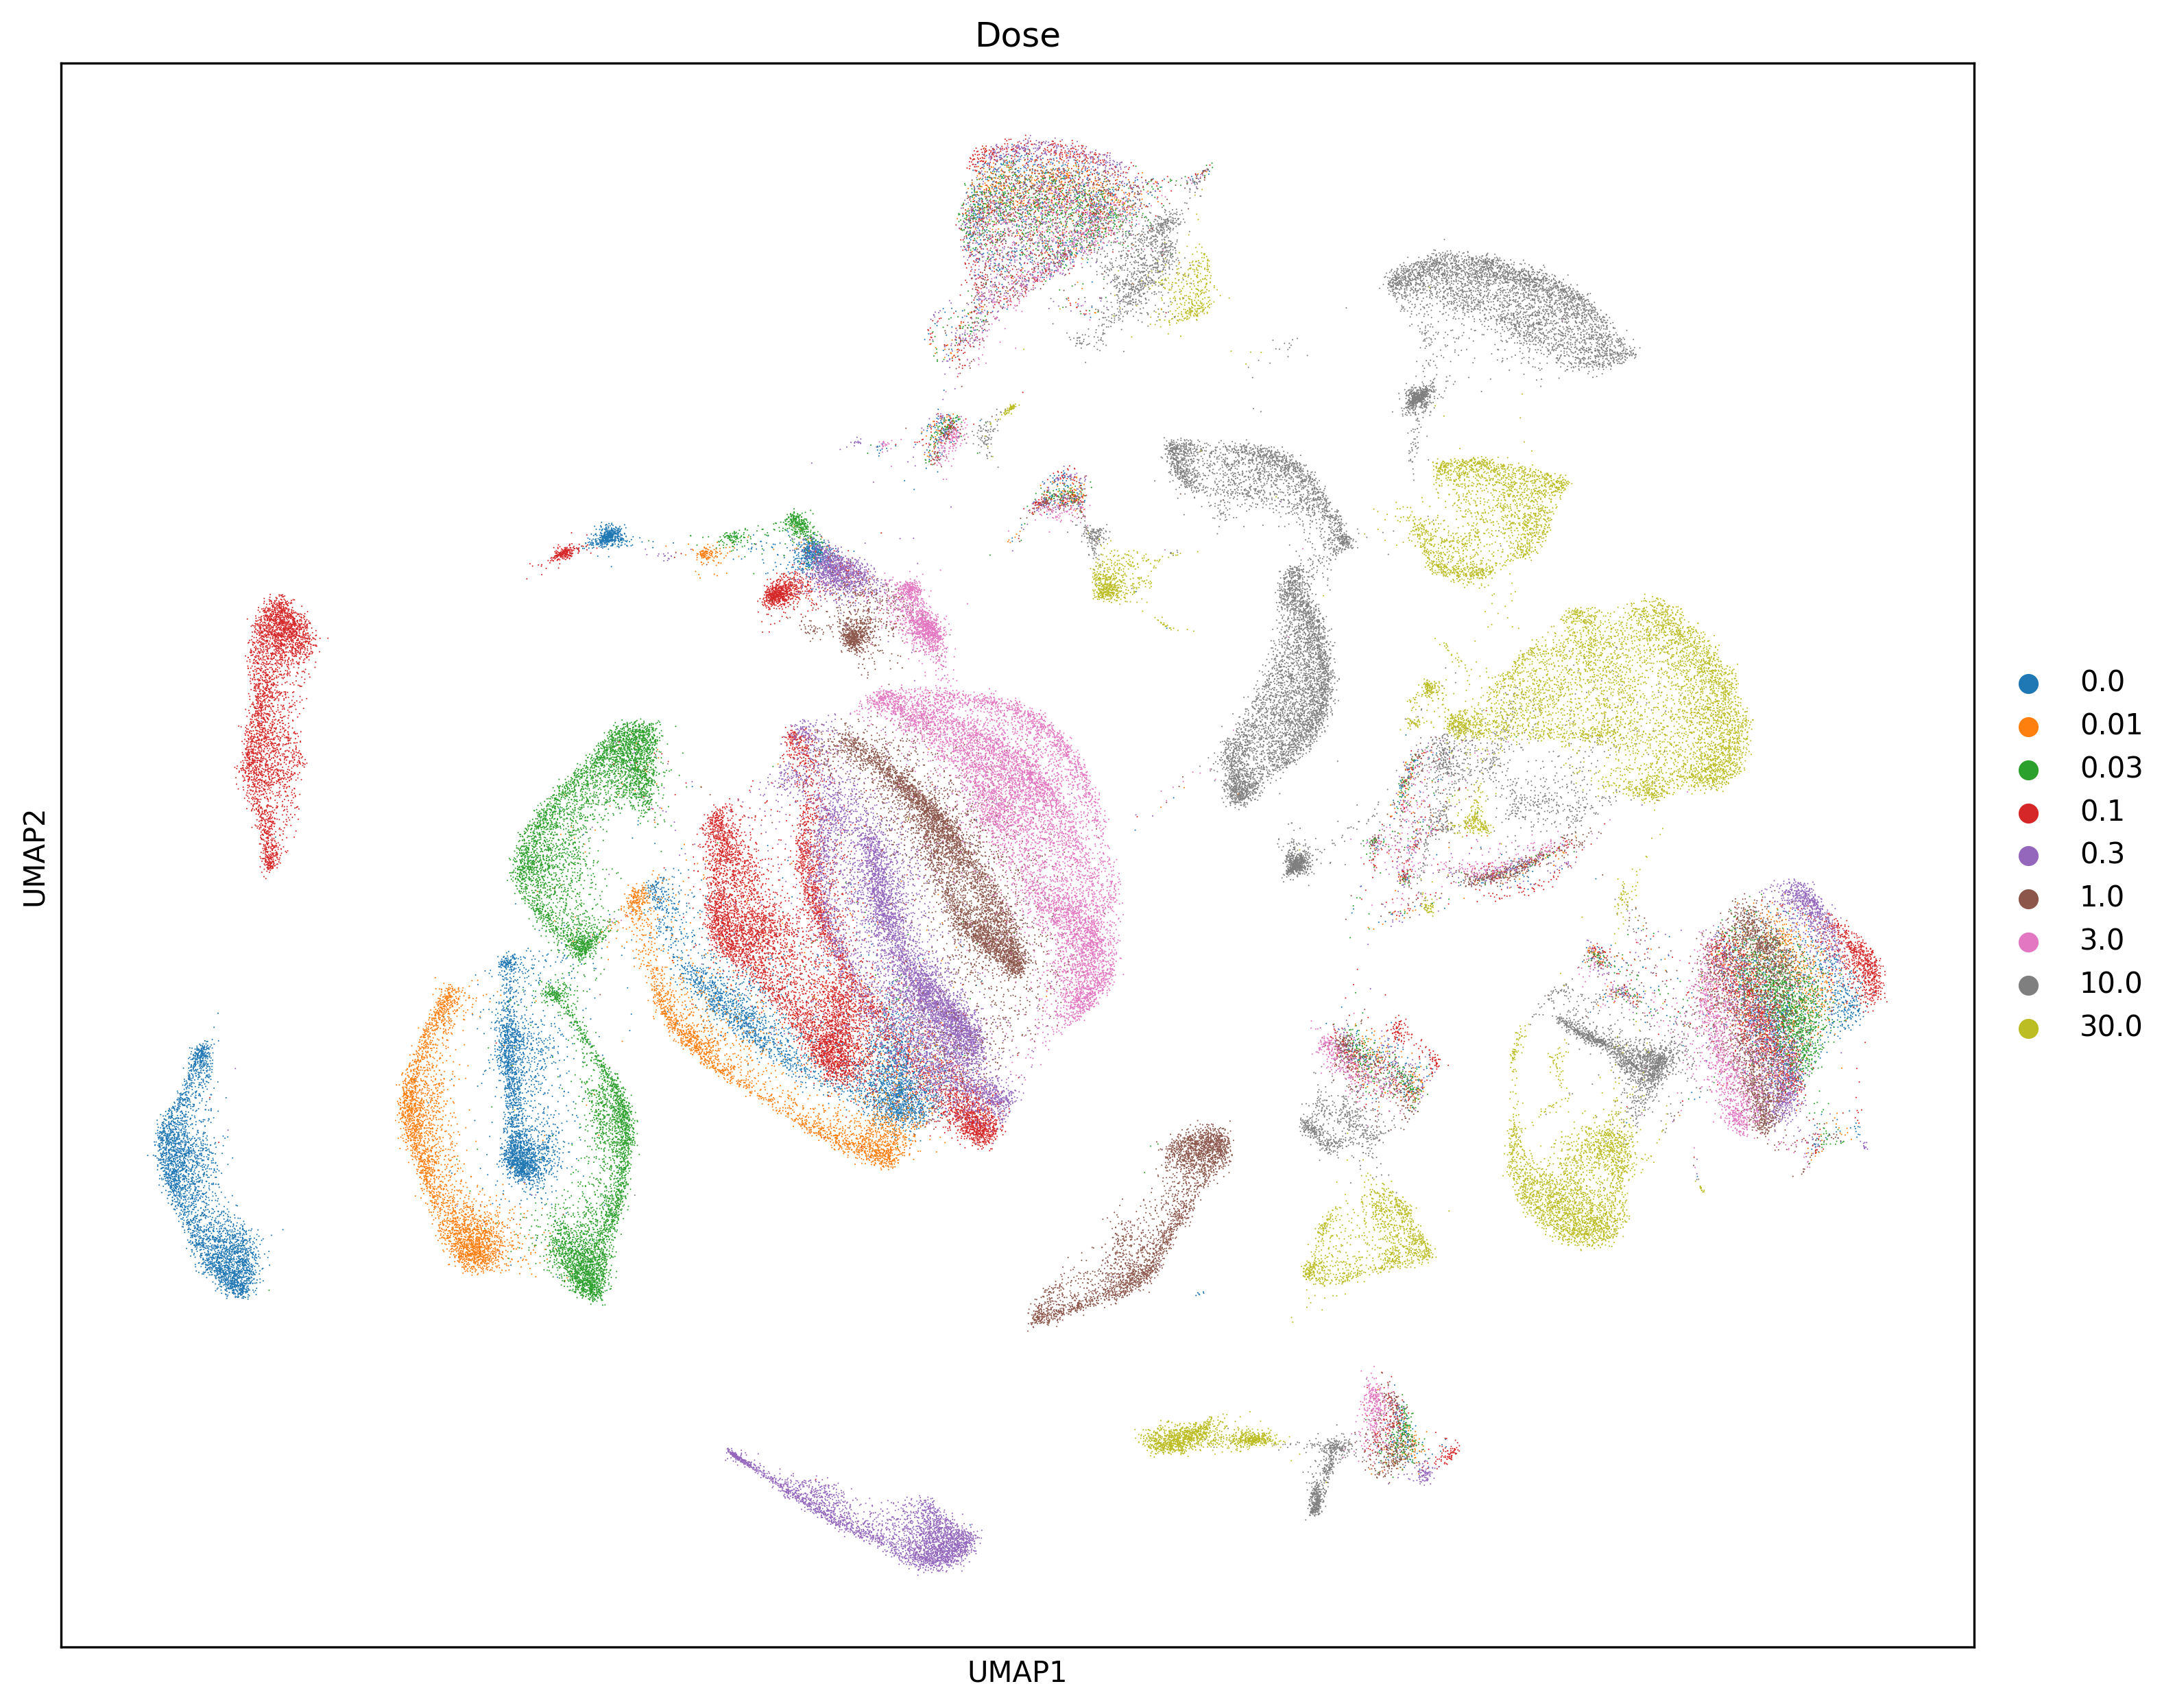
\includegraphics[width=.8\textwidth]{figures/nault_dose_umap.png}
        \caption{}
        \label{fig:figure2}
    \end{subfigure}%
    \hfill
    \begin{subfigure}[b]{\textwidth}
        \centering
        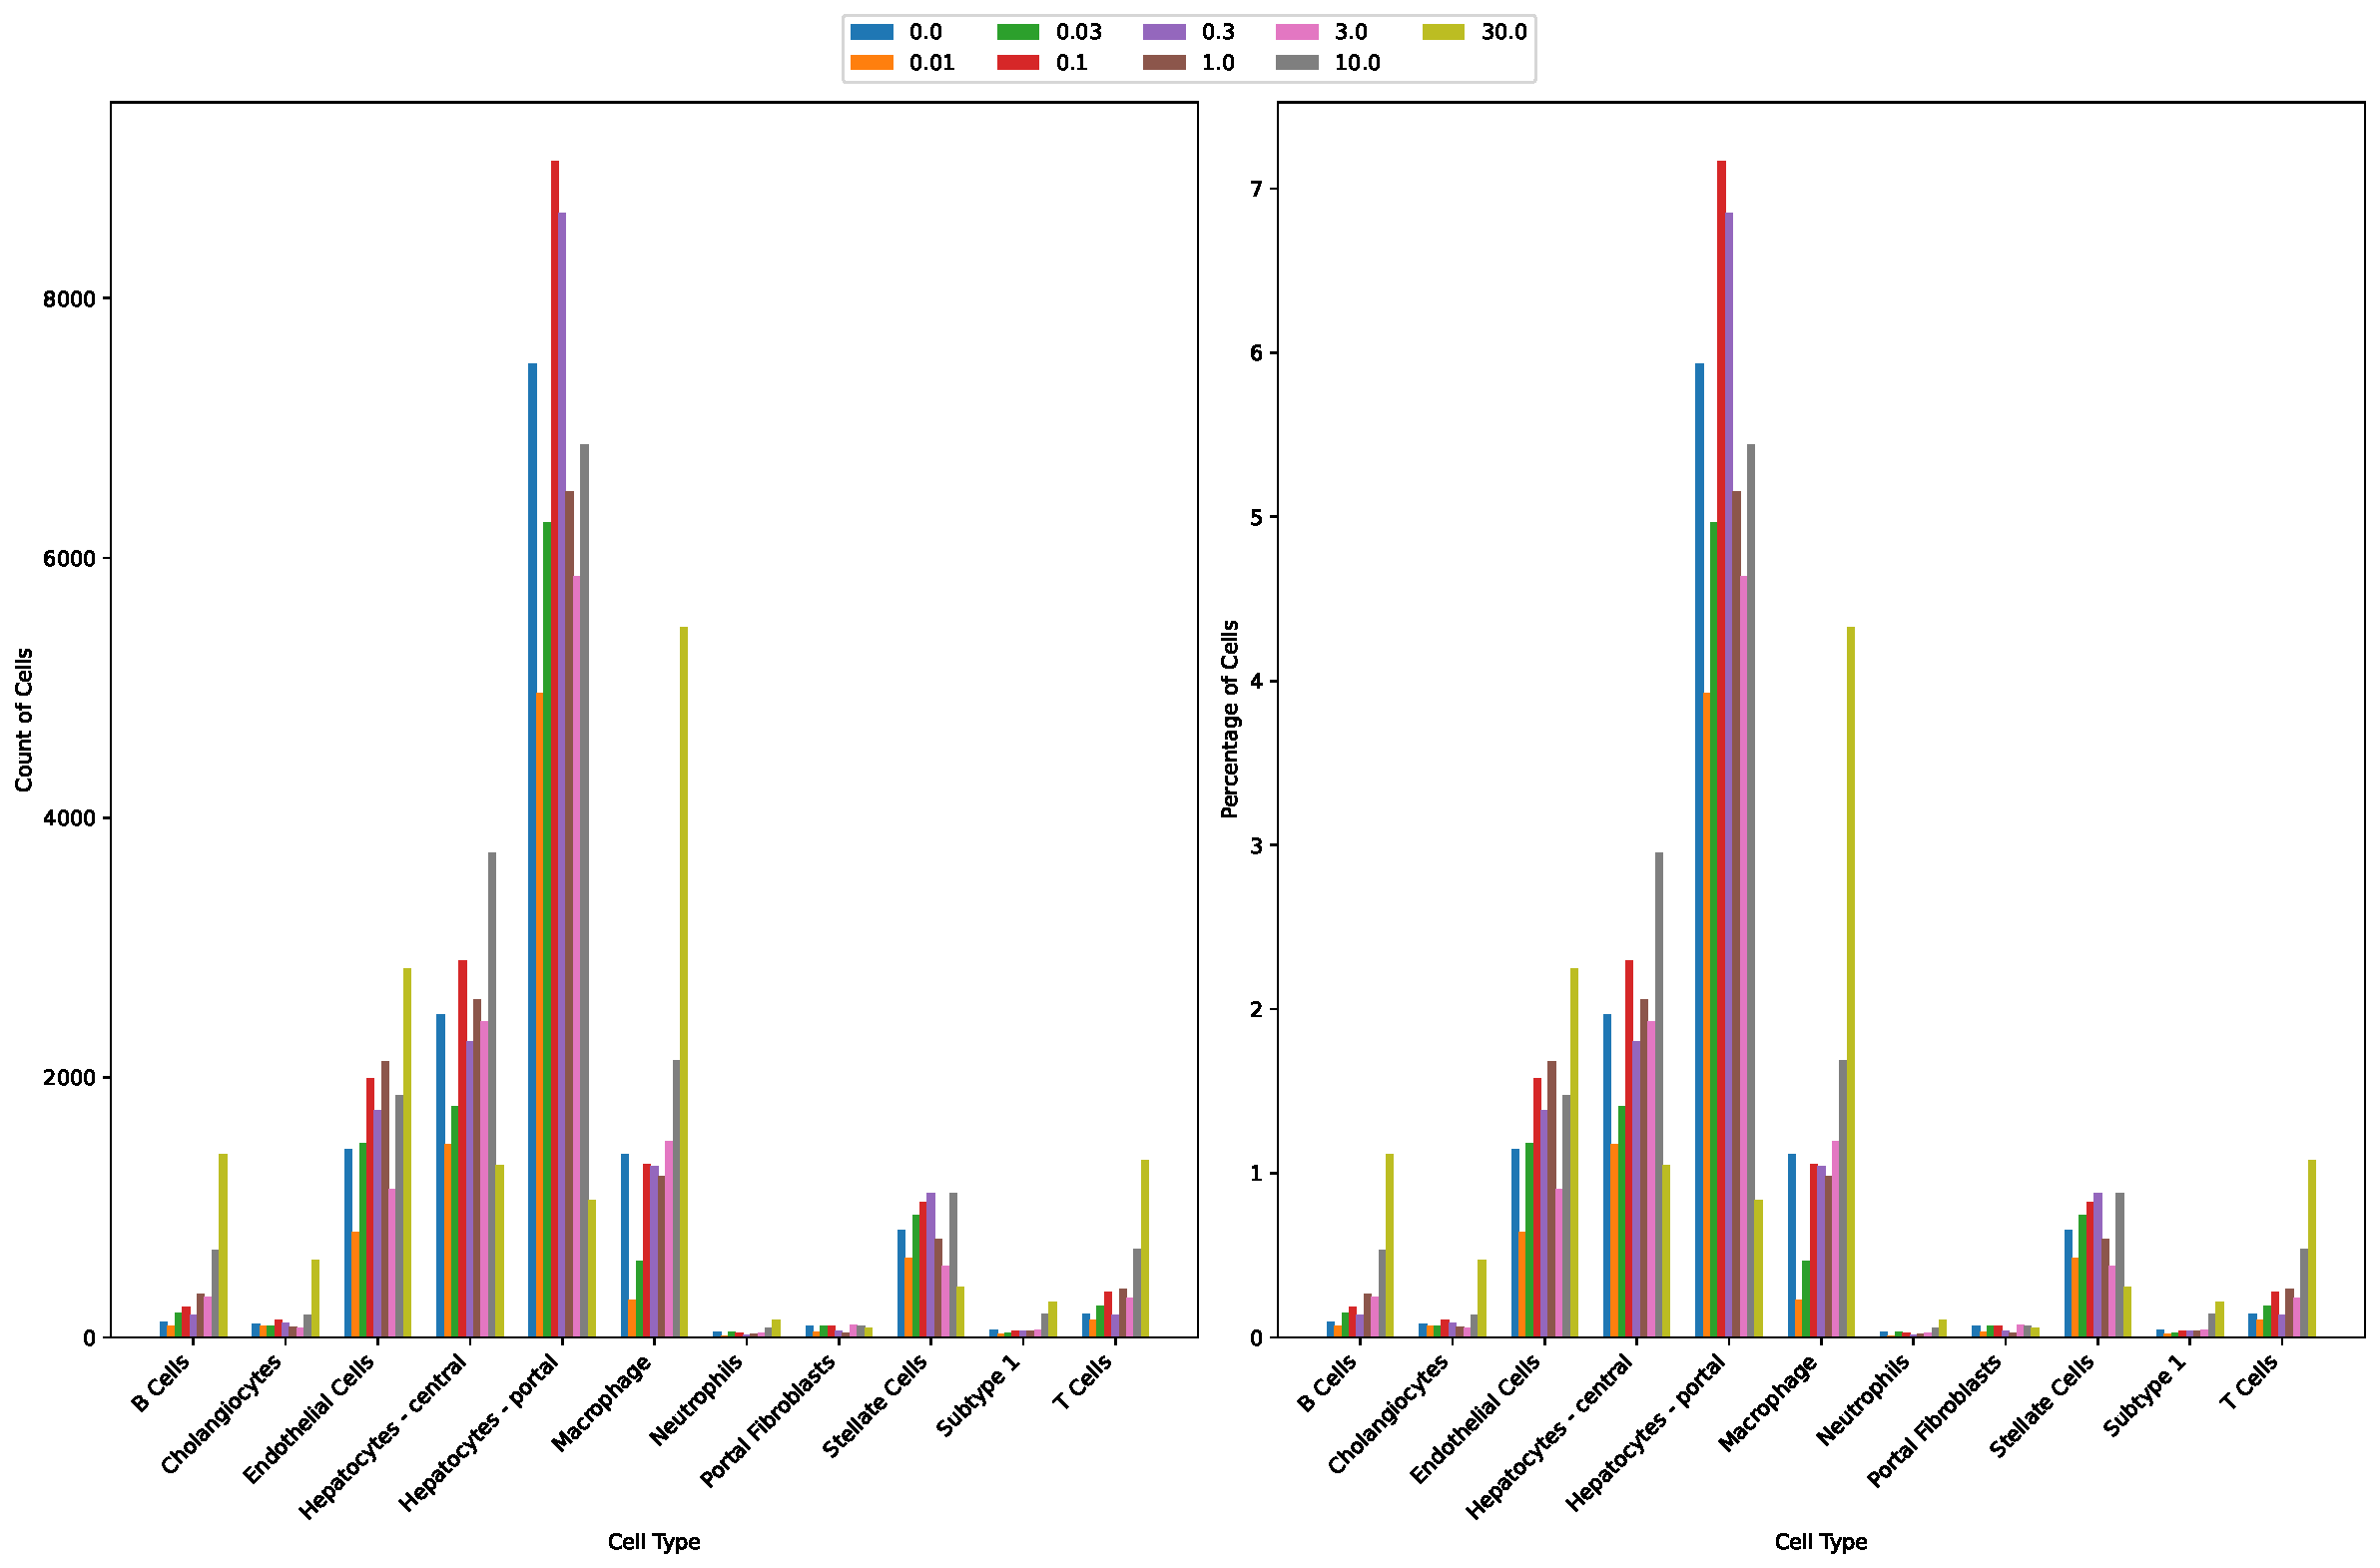
\includegraphics[width=.7\textwidth]{figures/nault_dosages_counts.pdf}
        \caption{}
        \label{fig:figure3}
    \end{subfigure}
    \hfill
    \begin{subfigure}[b]{\textwidth}
        \centering
        \includegraphics[width=.7\textwidth]{figures/nault_cell_types_counts.pdf}
        \caption{}
        \label{fig:figure4}
    \end{subfigure}    
    \caption{Nault overview}
    \label{fig:combined}
\end{figure}



\begin{figure}
    \centering
    \begin{minipage}{0.4\textwidth}
        \centering
        \includegraphics[width=\textwidth]{figures/nault_edistance_clustermap.pdf}
        \caption{E-distance}
    \end{minipage} \hfill
    \begin{minipage}{0.4\textwidth}
        \centering
        \includegraphics[width=\textwidth]{figures/nault_euclidean_clustermap.pdf}
        \caption{Euclidean}
    \end{minipage}
    \vskip\baselineskip

    \begin{minipage}{0.4\textwidth}
        \centering
        \includegraphics[width=\textwidth]{figures/nault_mean_pairwise_clustermap.pdf}
        \caption{Mean pairwise}
    \end{minipage} \hfill
    \begin{minipage}{0.4\textwidth}
        \centering
        \includegraphics[width=\textwidth]{figures/nault_mmd_clustermap.pdf}
        \caption{MMD}
    \end{minipage}
    \vskip\baselineskip

    \begin{minipage}{0.4\textwidth}
        \centering
        \includegraphics[width=\textwidth]{figures/nault_wasserstein_clustermap.pdf}
        \caption{Wasserstein}
    \end{minipage}
    \caption{Distance metrics across all cell types per dosage}
\end{figure}

\begin{figure}
    \centering
    \begin{minipage}{0.4\textwidth}
        \centering
        \includegraphics[width=\textwidth]{figures/hepatocytes_edistance_clustermap.pdf}
        \caption{E-distance}
    \end{minipage} \hfill
    \begin{minipage}{0.4\textwidth}
        \centering
        \includegraphics[width=\textwidth]{figures/hepatocytes_euclidean_clustermap.pdf}
        \caption{Euclidean}
    \end{minipage}
    \vskip\baselineskip

    \begin{minipage}{0.4\textwidth}
        \centering
        \includegraphics[width=\textwidth]{figures/hepatocytes_mean_pairwise_clustermap.pdf}
        \caption{Mean pairwise}
    \end{minipage} \hfill
    \begin{minipage}{0.4\textwidth}
        \centering
        \includegraphics[width=\textwidth]{figures/hepatocytes_mmd_clustermap.pdf}
        \caption{MMD}
    \end{minipage}
    \vskip\baselineskip

    \begin{minipage}{0.4\textwidth}
        \centering
        \includegraphics[width=\textwidth]{figures/hepatocytes_wasserstein_clustermap.pdf}
        \caption{Wasserstein}
    \end{minipage}
    \caption{Distance metrics for cell type Hepatocytes - portal per dosage}
\end{figure}

\begin{figure}
    \centering
    \begin{minipage}{0.4\textwidth}
        \centering
        \includegraphics[width=\textwidth]{figures/hepatocytes_central_edistance_clustermap.pdf}
        \caption{E-distance}
    \end{minipage} \hfill
    \begin{minipage}{0.4\textwidth}
        \centering
        \includegraphics[width=\textwidth]{figures/hepatocytes_central_euclidean_clustermap.pdf}
        \caption{Euclidean}
    \end{minipage}
    \vskip\baselineskip

    \begin{minipage}{0.4\textwidth}
        \centering
        \includegraphics[width=\textwidth]{figures/hepatocytes_central_mean_pairwise_clustermap.pdf}
        \caption{Mean pairwise}
    \end{minipage} \hfill
    \begin{minipage}{0.4\textwidth}
        \centering
        \includegraphics[width=\textwidth]{figures/hepatocytes_central_mmd_clustermap.pdf}
        \caption{MMD}
    \end{minipage}
    \vskip\baselineskip

    \begin{minipage}{0.4\textwidth}
        \centering
        \includegraphics[width=\textwidth]{figures/hepatocytes_central_wasserstein_clustermap.pdf}
        \caption{Wasserstein}
    \end{minipage}
    \caption{Distance metrics for cell type Hepatocytes - central per dosage}
\end{figure}

\begin{figure}
    \centering
    \begin{minipage}{0.4\textwidth}
        \centering
        \includegraphics[width=\textwidth]{figures/dose_highest_edistance_clustermap.pdf}
        \caption{E-distance}
    \end{minipage} \hfill
    \begin{minipage}{0.4\textwidth}
        \centering
        \includegraphics[width=\textwidth]{figures/dose_highest_euclidean_clustermap.pdf}
        \caption{Euclidean}
    \end{minipage}
    \vskip\baselineskip

    \begin{minipage}{0.4\textwidth}
        \centering
        \includegraphics[width=\textwidth]{figures/dose_highest_mean_pairwise_clustermap.pdf}
        \caption{Mean pairwise}
    \end{minipage} \hfill
    \begin{minipage}{0.4\textwidth}
        \centering
        \includegraphics[width=\textwidth]{figures/dose_highest_mmd_clustermap.pdf}
        \caption{MMD}
    \end{minipage}
    \vskip\baselineskip

    \begin{minipage}{0.4\textwidth}
        \centering
        \includegraphics[width=\textwidth]{figures/dose_highest_wasserstein_clustermap.pdf}
        \caption{Wasserstein}
    \end{minipage}
    \caption{Distance metrics for dosage highest 30 $\mu g/kg$ per cell type}
\end{figure}

\begin{figure}
    \centering
    \begin{minipage}{0.4\textwidth}
        \centering
        \includegraphics[width=\textwidth]{figures/dose_lowest_edistance_clustermap.pdf}
        \caption{E-distance}
    \end{minipage} \hfill
    \begin{minipage}{0.4\textwidth}
        \centering
        \includegraphics[width=\textwidth]{figures/dose_lowest_euclidean_clustermap.pdf}
        \caption{Euclidean}
    \end{minipage}
    \vskip\baselineskip

    \begin{minipage}{0.4\textwidth}
        \centering
        \includegraphics[width=\textwidth]{figures/dose_lowest_mean_pairwise_clustermap.pdf}
        \caption{Mean pairwise}
    \end{minipage} \hfill
    \begin{minipage}{0.4\textwidth}
        \centering
        \includegraphics[width=\textwidth]{figures/dose_lowest_mmd_clustermap.pdf}
        \caption{MMD}
    \end{minipage}
    \vskip\baselineskip

    \begin{minipage}{0.4\textwidth}
        \centering
        \includegraphics[width=\textwidth]{figures/dose_lowest_wasserstein_clustermap.pdf}
        \caption{Wasserstein}
    \end{minipage}
    \caption{Distance metrics for lowest dosage 0.01 $\mu g/kg$ per cell type}
\end{figure}

\clearpage


\subsection{PBMC dataset}


\begin{figure}[h]
    \centering
    \begin{subfigure}[t]{0.49\textwidth}
        \centering
        \includegraphics[width=\textwidth]{figures/pbmc_cell_umap.png}
        \caption{}
        \label{fig:figure1}
    \end{subfigure}
    \hfill
    \begin{subfigure}[t]{0.49\textwidth}
        \centering
        \includegraphics[width=.95\textwidth]{figures/pbmc_condtion_umap.png}
        \caption{}
        \label{fig:figure2}
    \end{subfigure}
    \hfill
    \begin{subfigure}[b]{\textwidth}
        \centering
        \includegraphics[width=.9\textwidth]{figures/pbmc_counts.pdf}
        \caption{}
        \label{fig:figure3}
    \end{subfigure}
    \caption{PBMC overview}
    \label{fig:combined}
\end{figure}

\clearpage

\begin{figure}
    \centering
    \begin{minipage}{0.4\textwidth}
        \centering
        \includegraphics[width=\textwidth]{figures/pbmc_condition_edistance_clustermap.pdf}
        \caption{E-distance}
    \end{minipage} \hfill
    \begin{minipage}{0.4\textwidth}
        \centering
        \includegraphics[width=\textwidth]{figures/pbmc_condition_euclidean_clustermap.pdf}
        \caption{Euclidean}
    \end{minipage}
    \vskip\baselineskip

    \begin{minipage}{0.4\textwidth}
        \centering
        \includegraphics[width=\textwidth]{figures/pbmc_condition_mean_pairwise_clustermap.pdf}
        \caption{Mean pairwise}
    \end{minipage} \hfill
    \begin{minipage}{0.4\textwidth}
        \centering
        \includegraphics[width=\textwidth]{figures/pbmc_condition_mmd_clustermap.pdf}
        \caption{MMD}
    \end{minipage}
    \vskip\baselineskip

    \begin{minipage}{0.4\textwidth}
        \centering
        \includegraphics[width=\textwidth]{figures/pbmc_condition_wasserstein_clustermap.pdf}
        \caption{Wasserstein}
    \end{minipage}
    \caption{Distance metrics per condition}
\end{figure}

\clearpage


\begin{figure}
    \centering
    \begin{minipage}{0.4\textwidth}
        \centering
        \includegraphics[width=\textwidth]{figures/pbmc_cell_type_edistance_clustermap.pdf}
        \caption{E-distance}
    \end{minipage} \hfill
    \begin{minipage}{0.4\textwidth}
        \centering
        \includegraphics[width=\textwidth]{figures/pbmc_cell_type_euclidean_clustermap.pdf}
        \caption{Euclidean}
    \end{minipage}
    \vskip\baselineskip

    \begin{minipage}{0.4\textwidth}
        \centering
        \includegraphics[width=\textwidth]{figures/pbmc_cell_type_mean_pairwise_clustermap.pdf}
        \caption{Mean pairwise}
    \end{minipage} \hfill
    \begin{minipage}{0.4\textwidth}
        \centering
        \includegraphics[width=\textwidth]{figures/pbmc_cell_type_mmd_clustermap.pdf}
        \caption{MMD}
    \end{minipage}
    \vskip\baselineskip

    \begin{minipage}{0.4\textwidth}
        \centering
        \includegraphics[width=\textwidth]{figures/pbmc_cell_type_wasserstein_clustermap.pdf}
        \caption{Wasserstein}
    \end{minipage}
    \caption{Distance metrics per cell type}
\end{figure}

\clearpage


\section{Nault all cell types evaluation}

\subsection{Multiple doses}

\begin{figure}[h!]
    \centering
    \includegraphics[width=.8\textwidth]{figures/nault_umap_split_multiple.png}
\end{figure}

\begin{figure}[h!]
    \centering
    \includegraphics[width=.8\textwidth]{figures/nault_bars_split_multiple.pdf}
\end{figure}


\subsection{Single dose}


\begin{figure}[h!]
    \centering
    \includegraphics[width=.7\textwidth]{figures/nault_umap_split_30.png}
    \caption{Example of $30 \mu g/kg$}
\end{figure}

\begin{figure}[h!]
    \centering
    \includegraphics[width=.7\textwidth]{figures/nault_bars_split_30.pdf}
    \caption{Number of cells per cell type for $30 \mu g/kg$}
\end{figure}

\clearpage


\subsection{Comparison}


\begin{figure}[h!]
    \centering
    \includegraphics[width=.8\textwidth]{figures/nault_30_baseline_metrics_bars.pdf}
    \caption{Baseline metrics for highest dosage $30 \mu g/kg$ across cell types}
\end{figure}

\begin{figure}[h!]
    \centering
    \includegraphics[width=.8\textwidth]{figures/nault_30_distance_metrics_bars.pdf}
    \caption{Distance metrics for highest dosage $30 \mu g/kg$ across cell types}
\end{figure}

\clearpage

\begin{figure}[h!]
    \centering
    \includegraphics[width=.8\textwidth]{figures/nault_01_baseline_metrics_bars.pdf}
    \caption{Baseline metrics for lowest dosage $0.01 \mu g/kg$ across cell types}
\end{figure}

\begin{figure}[h!]
    \centering
    \includegraphics[width=.8\textwidth]{figures/nault_01_distance_metrics_bars.pdf}
    \caption{Distance metrics for lowest dosage $0.01 \mu g/kg$ across cell types}
\end{figure}

\clearpage


\begin{figure}[h!]
    \centering
    \includegraphics[width=.8\textwidth]{figures/nault_hepatocytes_baseline_metrics_bars.pdf}
    \caption{Baseline metrics for Hepatocytes - portal across dosages}
\end{figure}

\begin{figure}[h!]
    \centering
    \includegraphics[width=.8\textwidth]{figures/nault_hepatocytes_distance_metrics_bars.pdf}
    \caption{Distance metrics for Hepatocytes - portal across dosages}
\end{figure}

\clearpage

\begin{figure}
    \centering
    \begin{minipage}{0.49\textwidth}
        \centering
        \includegraphics[width=\textwidth]{figures/3d_nault_DEGs.pdf}
        \caption{}
    \end{minipage} \hfill
    \begin{minipage}{0.49\textwidth}
        \centering
        \includegraphics[width=\textwidth]{figures/3d_nault_r2mean_all_boostrap_mean.pdf}
        \caption{}
    \end{minipage}
    \vskip\baselineskip

    \begin{minipage}{0.49\textwidth}
        \centering
        \includegraphics[width=\textwidth]{figures/3d_nault_r2mean_top20_boostrap_mean.pdf}
        \caption{}
    \end{minipage} \hfill
    \begin{minipage}{0.49\textwidth}
        \centering
        \includegraphics[width=\textwidth]{figures/3d_nault_r2mean_top100_boostrap_mean.pdf}
        \caption{}
    \end{minipage}
    \vskip\baselineskip
\end{figure}

\clearpage

\begin{figure}
    \centering
    \begin{minipage}{0.4\textwidth}
        \centering
        \includegraphics[width=\textwidth]{figures/3d_nault_edistance.pdf}
        \caption{E-distance}
    \end{minipage} \hfill
    \begin{minipage}{0.4\textwidth}
        \centering
        \includegraphics[width=\textwidth]{figures/3d_nault_euclidean.pdf}
        \caption{Euclidean}
    \end{minipage}
    \vskip\baselineskip

    \begin{minipage}{0.4\textwidth}
        \centering
        \includegraphics[width=\textwidth]{figures/3d_nault_mean_pairwise.pdf}
        \caption{Mean pairwise}
    \end{minipage} \hfill
    \begin{minipage}{0.4\textwidth}
        \centering
        \includegraphics[width=\textwidth]{figures/3d_nault_mmd.pdf}
        \caption{MMD}
    \end{minipage}
    \vskip\baselineskip

    \begin{minipage}{0.4\textwidth}
        \centering
        \includegraphics[width=\textwidth]{figures/3d_nault_wasserstein.pdf}
        \caption{Wasserstein}
    \end{minipage}
    \caption{Distance metrics per cell type}
\end{figure}

\clearpage


\begin{figure}[h!]
    \centering
    \includegraphics[width=.9\textwidth]{figures/NaultPipeline_X_Violin_metrics0.pdf}
\end{figure}

\begin{figure}[h!]
    \centering
    \includegraphics[width=.9\textwidth]{figures/NaultPipeline_X_Violin_metrics1.pdf}
\end{figure}

\clearpage

\begin{figure}[h!]
    \centering
    \includegraphics[width=.9\textwidth]{figures/NaultPipeline_X_Boxplot_metrics0.pdf}
\end{figure}

\begin{figure}[h!]
    \centering
    \includegraphics[width=.9\textwidth]{figures/NaultPipeline_X_Boxplot_metrics1.pdf}
\end{figure}

\clearpage

\begin{figure}[h!]
    \centering
    \includegraphics[width=.9\textwidth]{figures/NaultPipeline_Y_Violin_metrics0.pdf}
\end{figure}

\begin{figure}[h!]
    \centering
    \includegraphics[width=.9\textwidth]{figures/NaultPipeline_Y_Violin_metrics1.pdf}
\end{figure}

\clearpage

\begin{figure}[h!]
    \centering
    \includegraphics[width=.9\textwidth]{figures/NaultPipeline_Y_Boxplot_metrics0.pdf}
\end{figure}

\begin{figure}[h!]
    \centering
    \includegraphics[width=.9\textwidth]{figures/NaultPipeline_Y_Boxplot_metrics1.pdf}
\end{figure}

\clearpage

\begin{figure}[h!]
    \centering
    \includegraphics[width=.8\textwidth]{figures/nault_contour_DEGs.pdf}
    \caption{DEGs}
\end{figure}

\begin{figure}[h!]
    \centering
    \includegraphics[width=.8\textwidth]{figures/nault_contour_r2mean_all_boostrap_mean.pdf}
    \caption{r2 HVGs}
\end{figure}

\clearpage

\begin{figure}[h!]
    \centering
    \includegraphics[width=.8\textwidth]{figures/nault_contour_r2mean_top20_boostrap_mean.pdf}
    \caption{r2 top 20}
\end{figure}

\begin{figure}[h!]
    \centering
    \includegraphics[width=.8\textwidth]{figures/nault_contour_r2mean_top100_boostrap_mean.pdf}
    \caption{r2 top 100}
\end{figure}

\clearpage

\begin{figure}[h!]
    \centering
    \includegraphics[width=.8\textwidth]{figures/nault_contour_edistance.pdf}
    \caption{E-distance}
\end{figure}

\begin{figure}[h!]
    \centering
    \includegraphics[width=.8\textwidth]{figures/nault_contour_euclidean.pdf}
    \caption{Euclidean}
\end{figure}

\clearpage

\begin{figure}[h!]
    \centering
    \includegraphics[width=.8\textwidth]{figures/nault_contour_mean_pairwise.pdf}
    \caption{Mean pairwise}
\end{figure}

\begin{figure}[h!]
    \centering
    \includegraphics[width=.8\textwidth]{figures/nault_contour_mmd.pdf}
    \caption{MMD}
\end{figure}

\clearpage

\begin{figure}[h!]
    \centering
    \includegraphics[width=\textwidth]{figures/nault_contour_wasserstein.pdf}
    \caption{Wasserstein}
\end{figure}

\clearpage

\section{Nault liver cell types evaluation}


\subsection{Multiple doses}


\begin{figure}[h!]
    \centering
    \includegraphics[width=.8\textwidth]{figures/nault_liver_umap_split_multiple.png}
\end{figure}

\begin{figure}[h!]
    \centering
    \includegraphics[width=.8\textwidth]{figures/nault_liver_bars_split_multiple.pdf}
\end{figure}


\subsection{Single dose 30 $\mu g/kg$}

\begin{figure}[h!]
    \centering
    \includegraphics[width=.8\textwidth]{figures/nault_liver_umap_split_30.png}
\end{figure}

\begin{figure}[h!]
    \centering
    \includegraphics[width=.8\textwidth]{figures/nault_liver_bars_split_30.pdf}
\end{figure}


\clearpage

\subsection{Comparison}


\begin{figure}[h!]
    \centering
    \includegraphics[width=.8\textwidth]{figures/nault_liver_30_baseline_metrics_bars.pdf}
    \caption{Baseline metrics for highest dosage $30 \mu g/kg$ across cell types}
\end{figure}

\begin{figure}[h!]
    \centering
    \includegraphics[width=.8\textwidth]{figures/nault_liver_30_distance_metrics_bars.pdf}
    \caption{Distance metrics for highest dosage $30 \mu g/kg$ across cell types}
\end{figure}

\clearpage

\begin{figure}[h!]
    \centering
    \includegraphics[width=.8\textwidth]{figures/nault_liver_01_baseline_metrics_bars.pdf}
    \caption{Baseline metrics for highest dosage $0.1 \mu g/kg$ across cell types}
\end{figure}

\begin{figure}[h!]
    \centering
    \includegraphics[width=.8\textwidth]{figures/nault_liver_01_distance_metrics_bars.pdf}
    \caption{Distance metrics for highest dosage $0.1 \mu g/kg$ across cell types}
\end{figure}

\clearpage

\begin{figure}[h!]
    \centering
    \includegraphics[width=.8\textwidth]{figures/nault_liver_hepatocytes_baseline_metrics_bars.pdf}
    \caption{Baseline metrics for Hepatocytes - portal across dosages}
\end{figure}

\begin{figure}[h!]
    \centering
    \includegraphics[width=.8\textwidth]{figures/nault_liver_hepatocytes_distance_metrics_bars.pdf}
    \caption{Distance metrics for Hepatocytes - portal across dosages}
\end{figure}

\clearpage


\begin{figure}
    \centering
    \begin{minipage}{0.49\textwidth}
        \centering
        \includegraphics[width=\textwidth]{figures/3d_nault_liver_DEGs.pdf}
        \caption{}
    \end{minipage} \hfill
    \begin{minipage}{0.49\textwidth}
        \centering
        \includegraphics[width=\textwidth]{figures/3d_nault_liver_r2mean_all_boostrap_mean.pdf}
        \caption{}
    \end{minipage}
    \vskip\baselineskip

    \begin{minipage}{0.49\textwidth}
        \centering
        \includegraphics[width=\textwidth]{figures/3d_nault_liver_r2mean_top20_boostrap_mean.pdf}
        \caption{}
    \end{minipage} \hfill
    \begin{minipage}{0.49\textwidth}
        \centering
        \includegraphics[width=\textwidth]{figures/3d_nault_liver_r2mean_top100_boostrap_mean.pdf}
        \caption{}
    \end{minipage}
    \vskip\baselineskip
\end{figure}

\clearpage

\begin{figure}
    \centering
    \begin{minipage}{0.4\textwidth}
        \centering
        \includegraphics[width=\textwidth]{figures/3d_nault_liver_edistance.pdf}
        \caption{E-distance}
    \end{minipage} \hfill
    \begin{minipage}{0.4\textwidth}
        \centering
        \includegraphics[width=\textwidth]{figures/3d_nault_liver_euclidean.pdf}
        \caption{Euclidean}
    \end{minipage}
    \vskip\baselineskip

    \begin{minipage}{0.4\textwidth}
        \centering
        \includegraphics[width=\textwidth]{figures/3d_nault_liver_mean_pairwise.pdf}
        \caption{Mean pairwise}
    \end{minipage} \hfill
    \begin{minipage}{0.4\textwidth}
        \centering
        \includegraphics[width=\textwidth]{figures/3d_nault_liver_mmd.pdf}
        \caption{MMD}
    \end{minipage}
    \vskip\baselineskip

    \begin{minipage}{0.4\textwidth}
        \centering
        \includegraphics[width=\textwidth]{figures/3d_nault_liver_wasserstein.pdf}
        \caption{Wasserstein}
    \end{minipage}
    \caption{Distance metrics per cell type}
\end{figure}

\clearpage


\begin{figure}[h!]
    \centering
    \includegraphics[width=.9\textwidth]{figures/NaultLiverPipeline_X_Violin_metrics0.pdf}
\end{figure}

\begin{figure}[h!]
    \centering
    \includegraphics[width=.9\textwidth]{figures/NaultLiverPipeline_X_Violin_metrics1.pdf}
\end{figure}

\clearpage

\begin{figure}[h!]
    \centering
    \includegraphics[width=.9\textwidth]{figures/NaultLiverPipeline_X_Boxplot_metrics0.pdf}
\end{figure}

\begin{figure}[h!]
    \centering
    \includegraphics[width=.9\textwidth]{figures/NaultLiverPipeline_X_Boxplot_metrics1.pdf}
\end{figure}

\clearpage

\begin{figure}[h!]
    \centering
    \includegraphics[width=.9\textwidth]{figures/NaultLiverPipeline_Y_Violin_metrics0.pdf}
\end{figure}

\begin{figure}[h!]
    \centering
    \includegraphics[width=.9\textwidth]{figures/NaultLiverPipeline_Y_Violin_metrics1.pdf}
\end{figure}

\clearpage

\begin{figure}[h!]
    \centering
    \includegraphics[width=.9\textwidth]{figures/NaultLiverPipeline_Y_Boxplot_metrics0.pdf}
\end{figure}

\begin{figure}[h!]
    \centering
    \includegraphics[width=.9\textwidth]{figures/NaultLiverPipeline_Y_Boxplot_metrics1.pdf}
\end{figure}

\clearpage

\begin{figure}[h!]
    \centering
    \includegraphics[width=.8\textwidth]{figures/nault_liver_contour_DEGs.pdf}
    \caption{DEGs}
\end{figure}

\begin{figure}[h!]
    \centering
    \includegraphics[width=.8\textwidth]{figures/nault_liver_contour_r2mean_all_boostrap_mean.pdf}
    \caption{r2 HVGs}
\end{figure}

\clearpage

\begin{figure}[h!]
    \centering
    \includegraphics[width=.8\textwidth]{figures/nault_liver_contour_r2mean_top20_boostrap_mean.pdf}
    \caption{r2 top 20}
\end{figure}

\begin{figure}[h!]
    \centering
    \includegraphics[width=.8\textwidth]{figures/nault_liver_contour_r2mean_top100_boostrap_mean.pdf}
    \caption{r2 top 100}
\end{figure}

\clearpage

\begin{figure}[h!]
    \centering
    \includegraphics[width=.8\textwidth]{figures/nault_liver_contour_edistance.pdf}
    \caption{E-distance}
\end{figure}

\begin{figure}[h!]
    \centering
    \includegraphics[width=.8\textwidth]{figures/nault_liver_contour_euclidean.pdf}
\end{figure}

\clearpage

\begin{figure}[h!]
    \centering
    \includegraphics[width=.8\textwidth]{figures/nault_liver_contour_mean_pairwise.pdf}
    \caption{Mean pairwise}
\end{figure}

\begin{figure}[h!]
    \centering
    \includegraphics[width=.8\textwidth]{figures/nault_liver_contour_mmd.pdf}
    \caption{MMD}
\end{figure}

\clearpage

\begin{figure}[h!]
    \centering
    \includegraphics[width=\textwidth]{figures/nault_liver_contour_wasserstein.pdf}
    \caption{Wasserstein}
\end{figure}

\clearpage

\subsection{Παρατηρήσεις}

\begin{itemize}
    \itemsep -0.2em
    \item Το scButterfly και το scPreGan έχουν παρόμοια συμπεριφορά στις μετρικές και εμφανίζουν μεγάλη διακύμανση κατά μήκος των τύπων των κυττάρων και των δόσεων.
    \item Τα μοντέλα που έχουν ως βάση την αρχιτεκτονική του scGen (scVIDR, και οι παραλλαγές του), VAR και post-processing στο latent space, έχουν την υψηλότερη και πιο σταθερή απόδοση σε μετρικές του $R^2$, ωστόσο υστερούν στην καταμέτρηση των κοινών διαφοροποιήσιμων γονιδίων έκφρασης (DEGs).
\end{itemize}

\clearpage

\section{PBMC}


\begin{figure}[h!]
    \centering
    \includegraphics[width=.8\textwidth]{figures/pbmc_split.png}
\end{figure}

\begin{figure}[h!]
    \centering
    \includegraphics[width=.8\textwidth]{figures/pbmc_bars_split.pdf}
\end{figure}

\clearpage

\subsection{Comparison}

\begin{figure}[h!]
    \centering
    \includegraphics[width=.8\textwidth]{figures/pbmc_baseline_metrics_bars.pdf}
\end{figure}

\begin{figure}[h!]
    \centering
    \includegraphics[width=.8\textwidth]{figures/pbmc_distance_metrics_bars.pdf}
\end{figure}
\addcontentsline{toc}{section}{References}
\bibliographystyle{plain}
\bibliography{references.bib}


\appendix


\end{document}